\documentclass[twoside]{book}

% Packages required by doxygen
\usepackage{fixltx2e}
\usepackage{calc}
\usepackage{doxygen}
\usepackage[export]{adjustbox} % also loads graphicx
\usepackage{graphicx}
\usepackage[utf8]{inputenc}
\usepackage{makeidx}
\usepackage{multicol}
\usepackage{multirow}
\PassOptionsToPackage{warn}{textcomp}
\usepackage{textcomp}
\usepackage[nointegrals]{wasysym}
\usepackage[table]{xcolor}

% Font selection
\usepackage[T1]{fontenc}
\usepackage[scaled=.90]{helvet}
\usepackage{courier}
\usepackage{amssymb}
\usepackage{sectsty}
\renewcommand{\familydefault}{\sfdefault}
\allsectionsfont{%
  \fontseries{bc}\selectfont%
  \color{darkgray}%
}
\renewcommand{\DoxyLabelFont}{%
  \fontseries{bc}\selectfont%
  \color{darkgray}%
}
\newcommand{\+}{\discretionary{\mbox{\scriptsize$\hookleftarrow$}}{}{}}

% Page & text layout
\usepackage{geometry}
\geometry{%
  a4paper,%
  top=2.5cm,%
  bottom=2.5cm,%
  left=2.5cm,%
  right=2.5cm%
}
\tolerance=750
\hfuzz=15pt
\hbadness=750
\setlength{\emergencystretch}{15pt}
\setlength{\parindent}{0cm}
\setlength{\parskip}{0.2cm}
\makeatletter
\renewcommand{\paragraph}{%
  \@startsection{paragraph}{4}{0ex}{-1.0ex}{1.0ex}{%
    \normalfont\normalsize\bfseries\SS@parafont%
  }%
}
\renewcommand{\subparagraph}{%
  \@startsection{subparagraph}{5}{0ex}{-1.0ex}{1.0ex}{%
    \normalfont\normalsize\bfseries\SS@subparafont%
  }%
}
\makeatother

% Headers & footers
\usepackage{fancyhdr}
\pagestyle{fancyplain}
\fancyhead[LE]{\fancyplain{}{\bfseries\thepage}}
\fancyhead[CE]{\fancyplain{}{}}
\fancyhead[RE]{\fancyplain{}{\bfseries\leftmark}}
\fancyhead[LO]{\fancyplain{}{\bfseries\rightmark}}
\fancyhead[CO]{\fancyplain{}{}}
\fancyhead[RO]{\fancyplain{}{\bfseries\thepage}}
\fancyfoot[LE]{\fancyplain{}{}}
\fancyfoot[CE]{\fancyplain{}{}}
\fancyfoot[RE]{\fancyplain{}{\bfseries\scriptsize Generated on Fri Feb 24 2017 17\+:58\+:00 for My Project by Doxygen }}
\fancyfoot[LO]{\fancyplain{}{\bfseries\scriptsize Generated on Fri Feb 24 2017 17\+:58\+:00 for My Project by Doxygen }}
\fancyfoot[CO]{\fancyplain{}{}}
\fancyfoot[RO]{\fancyplain{}{}}
\renewcommand{\footrulewidth}{0.4pt}
\renewcommand{\chaptermark}[1]{%
  \markboth{#1}{}%
}
\renewcommand{\sectionmark}[1]{%
  \markright{\thesection\ #1}%
}

% Indices & bibliography
\usepackage{natbib}
\usepackage[titles]{tocloft}
\setcounter{tocdepth}{3}
\setcounter{secnumdepth}{5}
\makeindex

% Hyperlinks (required, but should be loaded last)
\usepackage{ifpdf}
\ifpdf
  \usepackage[pdftex,pagebackref=true]{hyperref}
\else
  \usepackage[ps2pdf,pagebackref=true]{hyperref}
\fi
\hypersetup{%
  colorlinks=true,%
  linkcolor=blue,%
  citecolor=blue,%
  unicode%
}

% Custom commands
\newcommand{\clearemptydoublepage}{%
  \newpage{\pagestyle{empty}\cleardoublepage}%
}


%===== C O N T E N T S =====

\begin{document}

% Titlepage & ToC
\hypersetup{pageanchor=false,
             bookmarks=true,
             bookmarksnumbered=true,
             pdfencoding=unicode
            }
\pagenumbering{roman}
\begin{titlepage}
\vspace*{7cm}
\begin{center}%
{\Large My Project }\\
\vspace*{1cm}
{\large Generated by Doxygen 1.8.10}\\
\vspace*{0.5cm}
{\small Fri Feb 24 2017 17:58:00}\\
\end{center}
\end{titlepage}
\clearemptydoublepage
\tableofcontents
\clearemptydoublepage
\pagenumbering{arabic}
\hypersetup{pageanchor=true}

%--- Begin generated contents ---
\chapter{Hierarchical Index}
\section{Class Hierarchy}
This inheritance list is sorted roughly, but not completely, alphabetically\+:\begin{DoxyCompactList}
\item \contentsline{section}{Arc\+\_\+t}{\pageref{struct_arc__t}}{}
\item \contentsline{section}{asfig}{\pageref{structasfig}}{}
\item \contentsline{section}{asisc}{\pageref{structasisc}}{}
\item \contentsline{section}{asiss}{\pageref{structasiss}}{}
\item \contentsline{section}{asobj}{\pageref{structasobj}}{}
\item \contentsline{section}{asosc}{\pageref{structasosc}}{}
\item \contentsline{section}{Basic\+\_\+block}{\pageref{class_basic__block}}{}
\item \contentsline{section}{Cfg}{\pageref{class_cfg}}{}
\item \contentsline{section}{dep}{\pageref{structdep}}{}
\item \contentsline{section}{Dfg}{\pageref{class_dfg}}{}
\item \contentsline{section}{Function}{\pageref{class_function}}{}
\item \contentsline{section}{Line}{\pageref{class_line}}{}
\begin{DoxyCompactList}
\item \contentsline{section}{Directive}{\pageref{class_directive}}{}
\item \contentsline{section}{Instruction}{\pageref{class_instruction}}{}
\item \contentsline{section}{Label}{\pageref{class_label}}{}
\end{DoxyCompactList}
\item \contentsline{section}{Node\+\_\+dfg}{\pageref{class_node__dfg}}{}
\item \contentsline{section}{Operand}{\pageref{class_operand}}{}
\begin{DoxyCompactList}
\item \contentsline{section}{O\+P\+Expression}{\pageref{class_o_p_expression}}{}
\item \contentsline{section}{O\+P\+Immediate}{\pageref{class_o_p_immediate}}{}
\item \contentsline{section}{O\+P\+Label}{\pageref{class_o_p_label}}{}
\item \contentsline{section}{O\+P\+Register}{\pageref{class_o_p_register}}{}
\end{DoxyCompactList}
\item \contentsline{section}{Program}{\pageref{class_program}}{}
\item \contentsline{section}{s\+\_\+\+Profile}{\pageref{structs___profile}}{}
\item Test\+Fixture\begin{DoxyCompactList}
\item \contentsline{section}{Test\+O\+P\+Label}{\pageref{class_test_o_p_label}}{}
\end{DoxyCompactList}
\item \contentsline{section}{utchn}{\pageref{structutchn}}{}
\item \contentsline{section}{utdat}{\pageref{unionutdat}}{}
\item \contentsline{section}{utdic}{\pageref{structutdic}}{}
\item \contentsline{section}{utdit}{\pageref{structutdit}}{}
\item \contentsline{section}{uttdc}{\pageref{structuttdc}}{}
\item \contentsline{section}{uttpd}{\pageref{structuttpd}}{}
\item \contentsline{section}{uttyp}{\pageref{structuttyp}}{}
\item \contentsline{section}{Y\+Y\+S\+T\+Y\+P\+E}{\pageref{union_y_y_s_t_y_p_e}}{}
\end{DoxyCompactList}

\chapter{Class Index}
\section{Class List}
Here are the classes, structs, unions and interfaces with brief descriptions\+:\begin{DoxyCompactList}
\item\contentsline{section}{\hyperlink{struct_arc__t}{Arc\+\_\+t} }{\pageref{struct_arc__t}}{}
\item\contentsline{section}{\hyperlink{structasfig}{asfig} }{\pageref{structasfig}}{}
\item\contentsline{section}{\hyperlink{structasisc}{asisc} }{\pageref{structasisc}}{}
\item\contentsline{section}{\hyperlink{structasiss}{asiss} }{\pageref{structasiss}}{}
\item\contentsline{section}{\hyperlink{structasobj}{asobj} }{\pageref{structasobj}}{}
\item\contentsline{section}{\hyperlink{structasosc}{asosc} }{\pageref{structasosc}}{}
\item\contentsline{section}{\hyperlink{class_basic__block}{Basic\+\_\+block} \\*Class representing a \hyperlink{class_basic__block}{Basic\+\_\+block} of a fonction }{\pageref{class_basic__block}}{}
\item\contentsline{section}{\hyperlink{class_cfg}{Cfg} \\*Class representing control flow graph }{\pageref{class_cfg}}{}
\item\contentsline{section}{\hyperlink{structdep}{dep} }{\pageref{structdep}}{}
\item\contentsline{section}{\hyperlink{class_dfg}{Dfg} \\*Class representing a \hyperlink{class_dfg}{Dfg} of a Basic block, a data flow graph that is to be used to calculate the critical path and schedule code }{\pageref{class_dfg}}{}
\item\contentsline{section}{\hyperlink{class_directive}{Directive} \\*Class representing an \hyperlink{class_directive}{Directive} herited by \hyperlink{class_line}{Line} }{\pageref{class_directive}}{}
\item\contentsline{section}{\hyperlink{class_function}{Function} \\*Class representing a \hyperlink{class_function}{Function} on a program }{\pageref{class_function}}{}
\item\contentsline{section}{\hyperlink{class_instruction}{Instruction} \\*Class representing an instruction which herited by \hyperlink{class_line}{Line} }{\pageref{class_instruction}}{}
\item\contentsline{section}{\hyperlink{class_label}{Label} \\*Class representing an \hyperlink{class_label}{Label} herited by \hyperlink{class_line}{Line} }{\pageref{class_label}}{}
\item\contentsline{section}{\hyperlink{class_line}{Line} \\*Abstract class representing an \hyperlink{class_line}{Line} }{\pageref{class_line}}{}
\item\contentsline{section}{\hyperlink{class_node__dfg}{Node\+\_\+dfg} \\*Class representing a node of data flow graph }{\pageref{class_node__dfg}}{}
\item\contentsline{section}{\hyperlink{class_operand}{Operand} \\*Abstract class representing an operand }{\pageref{class_operand}}{}
\item\contentsline{section}{\hyperlink{class_o_p_expression}{O\+P\+Expression} \\*Class representing an expression herited by \hyperlink{class_operand}{Operand} }{\pageref{class_o_p_expression}}{}
\item\contentsline{section}{\hyperlink{class_o_p_immediate}{O\+P\+Immediate} \\*Class representing an Immediate herited by \hyperlink{class_operand}{Operand} }{\pageref{class_o_p_immediate}}{}
\item\contentsline{section}{\hyperlink{class_o_p_label}{O\+P\+Label} \\*Class representing a \hyperlink{class_label}{Label} herited by \hyperlink{class_operand}{Operand} }{\pageref{class_o_p_label}}{}
\item\contentsline{section}{\hyperlink{class_o_p_register}{O\+P\+Register} \\*Class representing a Register herited by \hyperlink{class_operand}{Operand} }{\pageref{class_o_p_register}}{}
\item\contentsline{section}{\hyperlink{class_program}{Program} \\*Class representing a program as list }{\pageref{class_program}}{}
\item\contentsline{section}{\hyperlink{structs___profile}{s\+\_\+\+Profile} \\*Structure allowing to add caracteristics to an operator }{\pageref{structs___profile}}{}
\item\contentsline{section}{\hyperlink{class_test_o_p_label}{Test\+O\+P\+Label} }{\pageref{class_test_o_p_label}}{}
\item\contentsline{section}{\hyperlink{structutchn}{utchn} }{\pageref{structutchn}}{}
\item\contentsline{section}{\hyperlink{unionutdat}{utdat} }{\pageref{unionutdat}}{}
\item\contentsline{section}{\hyperlink{structutdic}{utdic} }{\pageref{structutdic}}{}
\item\contentsline{section}{\hyperlink{structutdit}{utdit} }{\pageref{structutdit}}{}
\item\contentsline{section}{\hyperlink{structuttdc}{uttdc} }{\pageref{structuttdc}}{}
\item\contentsline{section}{\hyperlink{structuttpd}{uttpd} }{\pageref{structuttpd}}{}
\item\contentsline{section}{\hyperlink{structuttyp}{uttyp} }{\pageref{structuttyp}}{}
\item\contentsline{section}{\hyperlink{union_y_y_s_t_y_p_e}{Y\+Y\+S\+T\+Y\+P\+E} }{\pageref{union_y_y_s_t_y_p_e}}{}
\end{DoxyCompactList}

\chapter{File Index}
\section{File List}
Here is a list of all documented files with brief descriptions\+:\begin{DoxyCompactList}
\item\contentsline{section}{{\bfseries asm200.\+h} }{\pageref{asm200_8h}}{}
\item\contentsline{section}{{\bfseries asm\+\_\+mipsyac.\+h} }{\pageref{asm__mipsyac_8h}}{}
\item\contentsline{section}{\hyperlink{_basic__block_8h}{Basic\+\_\+block.\+h} \\*\hyperlink{class_basic__block}{Basic\+\_\+block} class }{\pageref{_basic__block_8h}}{}
\item\contentsline{section}{\hyperlink{_cfg_8h}{Cfg.\+h} \\*\hyperlink{class_cfg}{Cfg} class }{\pageref{_cfg_8h}}{}
\item\contentsline{section}{\hyperlink{_dfg_8h}{Dfg.\+h} \\*\hyperlink{class_dfg}{Dfg} class }{\pageref{_dfg_8h}}{}
\item\contentsline{section}{\hyperlink{_directive_8h}{Directive.\+h} \\*\hyperlink{class_directive}{Directive} class }{\pageref{_directive_8h}}{}
\item\contentsline{section}{{\bfseries Enum\+\_\+type.\+h} }{\pageref{_enum__type_8h}}{}
\item\contentsline{section}{\hyperlink{_function_8h}{Function.\+h} \\*\hyperlink{class_function}{Function} class }{\pageref{_function_8h}}{}
\item\contentsline{section}{\hyperlink{_instruction_8h}{Instruction.\+h} \\*\hyperlink{class_instruction}{Instruction} class }{\pageref{_instruction_8h}}{}
\item\contentsline{section}{\hyperlink{_label_8h}{Label.\+h} \\*\hyperlink{class_label}{Label} class }{\pageref{_label_8h}}{}
\item\contentsline{section}{\hyperlink{_line_8h}{Line.\+h} \\*\hyperlink{class_line}{Line} class }{\pageref{_line_8h}}{}
\item\contentsline{section}{\hyperlink{_node__dfg_8h}{Node\+\_\+dfg.\+h} \\*\hyperlink{class_node__dfg}{Node\+\_\+dfg} class }{\pageref{_node__dfg_8h}}{}
\item\contentsline{section}{\hyperlink{_operand_8h}{Operand.\+h} \\*\hyperlink{class_operand}{Operand} class }{\pageref{_operand_8h}}{}
\item\contentsline{section}{\hyperlink{_o_p_expression_8h}{O\+P\+Expression.\+h} \\*\hyperlink{class_o_p_expression}{O\+P\+Expression} class }{\pageref{_o_p_expression_8h}}{}
\item\contentsline{section}{\hyperlink{_o_p_immediate_8h}{O\+P\+Immediate.\+h} \\*\hyperlink{class_o_p_immediate}{O\+P\+Immediate} class }{\pageref{_o_p_immediate_8h}}{}
\item\contentsline{section}{\hyperlink{_o_p_label_8h}{O\+P\+Label.\+h} \\*\hyperlink{class_o_p_label}{O\+P\+Label} class }{\pageref{_o_p_label_8h}}{}
\item\contentsline{section}{\hyperlink{_o_p_register_8h}{O\+P\+Register.\+h} \\*\hyperlink{class_o_p_register}{O\+P\+Register} class }{\pageref{_o_p_register_8h}}{}
\item\contentsline{section}{\hyperlink{_program_8h}{Program.\+h} \\*\hyperlink{class_program}{Program} class }{\pageref{_program_8h}}{}
\item\contentsline{section}{{\bfseries Test\+O\+P\+Label.\+h} }{\pageref{_test_o_p_label_8h}}{}
\item\contentsline{section}{{\bfseries utl200.\+h} }{\pageref{utl200_8h}}{}
\end{DoxyCompactList}

\chapter{Class Documentation}
\hypertarget{struct_arc__t}{}\section{Arc\+\_\+t Struct Reference}
\label{struct_arc__t}\index{Arc\+\_\+t@{Arc\+\_\+t}}
\subsection*{Public Attributes}
\begin{DoxyCompactItemize}
\item 
\hypertarget{struct_arc__t_a629d4a4e9c44aae452c7d54979c82abe}{}int {\bfseries delai}\label{struct_arc__t_a629d4a4e9c44aae452c7d54979c82abe}

\item 
\hypertarget{struct_arc__t_a75234bf2ed3084da0bf5b8fbc52fdc67}{}t\+\_\+\+Dep {\bfseries dep}\label{struct_arc__t_a75234bf2ed3084da0bf5b8fbc52fdc67}

\item 
\hypertarget{struct_arc__t_af7eaf6285792517ed5f06eba6abe3211}{}\hyperlink{class_node__dfg}{Node\+\_\+dfg} $\ast$ {\bfseries next}\label{struct_arc__t_af7eaf6285792517ed5f06eba6abe3211}

\end{DoxyCompactItemize}


The documentation for this struct was generated from the following file\+:\begin{DoxyCompactItemize}
\item 
\hyperlink{_node__dfg_8h}{Node\+\_\+dfg.\+h}\end{DoxyCompactItemize}

\hypertarget{structasfig}{}\section{asfig Struct Reference}
\label{structasfig}\index{asfig@{asfig}}
\subsection*{Public Attributes}
\begin{DoxyCompactItemize}
\item 
\hypertarget{structasfig_acb2f83dbe7a1e3cc29529820c2d84f08}{}struct \hyperlink{structutdic}{utdic} $\ast$ {\bfseries G\+L\+B\+\_\+\+D\+I\+C}\label{structasfig_acb2f83dbe7a1e3cc29529820c2d84f08}

\item 
\hypertarget{structasfig_a0d08a06c7ef0d7d128b068e63ec65a08}{}struct \hyperlink{structuttyp}{uttyp} $\ast$ {\bfseries G\+L\+B\+\_\+\+S\+Y\+M}\label{structasfig_a0d08a06c7ef0d7d128b068e63ec65a08}

\item 
\hypertarget{structasfig_ae87202e68aa58ff7cf9d39b476d81d13}{}struct \hyperlink{structuttyp}{uttyp} $\ast$ {\bfseries M\+E\+M\+\_\+\+T\+A\+B}\label{structasfig_ae87202e68aa58ff7cf9d39b476d81d13}

\item 
\hypertarget{structasfig_a29babddc26cd0b8fec9c3c139dd78206}{}struct \hyperlink{structasosc}{asosc} $\ast$ {\bfseries O\+U\+T\+\_\+\+S\+E\+C}\label{structasfig_a29babddc26cd0b8fec9c3c139dd78206}

\item 
\hypertarget{structasfig_acdd790bc6a90c1a53d9c96d651d515ae}{}struct \hyperlink{structasisc}{asisc} $\ast$ {\bfseries I\+N\+\_\+\+S\+E\+C}\label{structasfig_acdd790bc6a90c1a53d9c96d651d515ae}

\item 
\hypertarget{structasfig_a7811bcfbf0a2fd6c47b0f457875d1379}{}struct \hyperlink{structasobj}{asobj} $\ast$ {\bfseries O\+B\+J\+E\+C\+T\+S}\label{structasfig_a7811bcfbf0a2fd6c47b0f457875d1379}

\item 
\hypertarget{structasfig_aef8acd1ebd4a06c7be326a16a3d587fc}{}unsigned int {\bfseries F\+L\+A\+G}\label{structasfig_aef8acd1ebd4a06c7be326a16a3d587fc}

\end{DoxyCompactItemize}


The documentation for this struct was generated from the following file\+:\begin{DoxyCompactItemize}
\item 
asm200.\+h\end{DoxyCompactItemize}

\hypertarget{structasisc}{}\section{asisc Struct Reference}
\label{structasisc}\index{asisc@{asisc}}
\subsection*{Public Attributes}
\begin{DoxyCompactItemize}
\item 
\hypertarget{structasisc_ad9e1171351b4def0dee34a931bef06c2}{}struct \hyperlink{structasisc}{asisc} $\ast$ {\bfseries N\+E\+X\+T}\label{structasisc_ad9e1171351b4def0dee34a931bef06c2}

\item 
\hypertarget{structasisc_a556fa34f54b5c9c75dd76650538afc1d}{}char $\ast$ {\bfseries I\+D\+E\+N\+T}\label{structasisc_a556fa34f54b5c9c75dd76650538afc1d}

\item 
\hypertarget{structasisc_a719068c36a0e9705bf73ee2f073c423d}{}struct \hyperlink{structasosc}{asosc} $\ast$ {\bfseries O\+U\+T\+\_\+\+S\+E\+C}\label{structasisc_a719068c36a0e9705bf73ee2f073c423d}

\item 
\hypertarget{structasisc_a2d489dd1bf43e16f31806a7e22b4c944}{}unsigned int {\bfseries P\+O\+S\+I\+T\+I\+O\+N}\label{structasisc_a2d489dd1bf43e16f31806a7e22b4c944}

\item 
\hypertarget{structasisc_acbc421dc86cceaf4736c520ab2380d76}{}unsigned int {\bfseries F\+L\+A\+G}\label{structasisc_acbc421dc86cceaf4736c520ab2380d76}

\end{DoxyCompactItemize}


The documentation for this struct was generated from the following file\+:\begin{DoxyCompactItemize}
\item 
asm200.\+h\end{DoxyCompactItemize}

\hypertarget{structasiss}{}\section{asiss Struct Reference}
\label{structasiss}\index{asiss@{asiss}}
\subsection*{Public Attributes}
\begin{DoxyCompactItemize}
\item 
\hypertarget{structasiss_a68628730acb005ea7f11ea68de1d0548}{}struct \hyperlink{structasiss}{asiss} $\ast$ {\bfseries N\+E\+X\+T}\label{structasiss_a68628730acb005ea7f11ea68de1d0548}

\item 
\hypertarget{structasiss_a80a8a734b96c46174e20eafa5fd2858b}{}unsigned int {\bfseries A\+D\+D\+R}\label{structasiss_a80a8a734b96c46174e20eafa5fd2858b}

\item 
\hypertarget{structasiss_ae165bd0b21aa1165d33a69e641103589}{}unsigned int {\bfseries S\+I\+Z\+E}\label{structasiss_ae165bd0b21aa1165d33a69e641103589}

\item 
\hypertarget{structasiss_a359354e07893109790b9d08a4abd01ad}{}unsigned int {\bfseries F\+L\+A\+G}\label{structasiss_a359354e07893109790b9d08a4abd01ad}

\end{DoxyCompactItemize}


The documentation for this struct was generated from the following file\+:\begin{DoxyCompactItemize}
\item 
asm200.\+h\end{DoxyCompactItemize}

\hypertarget{structasobj}{}\section{asobj Struct Reference}
\label{structasobj}\index{asobj@{asobj}}
\subsection*{Public Attributes}
\begin{DoxyCompactItemize}
\item 
\hypertarget{structasobj_a9640c87bee0faf9f3f4e27464446b7dd}{}struct \hyperlink{structasobj}{asobj} $\ast$ {\bfseries N\+E\+X\+T}\label{structasobj_a9640c87bee0faf9f3f4e27464446b7dd}

\item 
\hypertarget{structasobj_ac3a92c991065cf1151dbe25b5db8166c}{}char $\ast$ {\bfseries I\+D\+E\+N\+T}\label{structasobj_ac3a92c991065cf1151dbe25b5db8166c}

\item 
\hypertarget{structasobj_ae2c40a301646b04f58c3176b2059aa3f}{}struct \hyperlink{structutdic}{utdic} $\ast$ {\bfseries S\+Y\+M\+\_\+\+D\+I\+C}\label{structasobj_ae2c40a301646b04f58c3176b2059aa3f}

\item 
\hypertarget{structasobj_a0af182b30fad283aa3dbb32fa02f368b}{}struct \hyperlink{structuttyp}{uttyp} $\ast$ {\bfseries S\+E\+C\+\_\+\+S\+Y\+M}\label{structasobj_a0af182b30fad283aa3dbb32fa02f368b}

\item 
\hypertarget{structasobj_aabba21bee06e84d00e257ac15339fcf3}{}unsigned int {\bfseries F\+L\+A\+G}\label{structasobj_aabba21bee06e84d00e257ac15339fcf3}

\end{DoxyCompactItemize}


The documentation for this struct was generated from the following file\+:\begin{DoxyCompactItemize}
\item 
asm200.\+h\end{DoxyCompactItemize}

\hypertarget{structasosc}{}\section{asosc Struct Reference}
\label{structasosc}\index{asosc@{asosc}}
\subsection*{Public Attributes}
\begin{DoxyCompactItemize}
\item 
\hypertarget{structasosc_a7ee21b53000a550b8aefb67b1c6e5f7f}{}struct \hyperlink{structasosc}{asosc} $\ast$ {\bfseries N\+E\+X\+T}\label{structasosc_a7ee21b53000a550b8aefb67b1c6e5f7f}

\item 
\hypertarget{structasosc_afc8abd23436b76f81cefb8aba492ead0}{}char $\ast$ {\bfseries I\+D\+E\+N\+T}\label{structasosc_afc8abd23436b76f81cefb8aba492ead0}

\item 
\hypertarget{structasosc_a71acd15a4ac27fe271378a7ee411a703}{}unsigned int {\bfseries I\+N\+S\+\_\+\+N\+B\+R}\label{structasosc_a71acd15a4ac27fe271378a7ee411a703}

\item 
\hypertarget{structasosc_a9839e2ff30cb42d4d0318b5ac52c1814}{}struct \hyperlink{structasiss}{asiss} $\ast$$\ast$ {\bfseries C\+U\+R\+\_\+\+I\+S\+S}\label{structasosc_a9839e2ff30cb42d4d0318b5ac52c1814}

\item 
\hypertarget{structasosc_abc1c84286924d8ea3a97a9374976d156}{}struct \hyperlink{structasiss}{asiss} $\ast$$\ast$ {\bfseries S\+U\+B\+\_\+\+S\+E\+C}\label{structasosc_abc1c84286924d8ea3a97a9374976d156}

\item 
\hypertarget{structasosc_a9a384f8d9c03da521e36b2003ea20449}{}unsigned int {\bfseries A\+D\+D\+R}\label{structasosc_a9a384f8d9c03da521e36b2003ea20449}

\item 
\hypertarget{structasosc_ab773c8a752c81f2d9b8dc9125541d3d0}{}unsigned int {\bfseries S\+I\+Z\+E}\label{structasosc_ab773c8a752c81f2d9b8dc9125541d3d0}

\item 
\hypertarget{structasosc_aa23f9d9016f7e5b295eb4dc2e957ad2c}{}unsigned int {\bfseries F\+L\+A\+G}\label{structasosc_aa23f9d9016f7e5b295eb4dc2e957ad2c}

\end{DoxyCompactItemize}


The documentation for this struct was generated from the following file\+:\begin{DoxyCompactItemize}
\item 
asm200.\+h\end{DoxyCompactItemize}

\hypertarget{class_basic__block}{}\section{Basic\+\_\+block Class Reference}
\label{class_basic__block}\index{Basic\+\_\+block@{Basic\+\_\+block}}


class representing a \hyperlink{class_basic__block}{Basic\+\_\+block} of a fonction  




{\ttfamily \#include $<$Basic\+\_\+block.\+h$>$}

\subsection*{Public Member Functions}
\begin{DoxyCompactItemize}
\item 
\hypertarget{class_basic__block_aa2455e1b1b8f5ac9b1c128f121fe3d67}{}\hyperlink{class_basic__block_aa2455e1b1b8f5ac9b1c128f121fe3d67}{Basic\+\_\+block} ()\label{class_basic__block_aa2455e1b1b8f5ac9b1c128f121fe3d67}

\begin{DoxyCompactList}\small\item\em Constructor of a Basic Block. \end{DoxyCompactList}\item 
\hypertarget{class_basic__block_a0047b58d9a30fa6eb79a87c70e9176d0}{}\hyperlink{class_basic__block_a0047b58d9a30fa6eb79a87c70e9176d0}{$\sim$\+Basic\+\_\+block} ()\label{class_basic__block_a0047b58d9a30fa6eb79a87c70e9176d0}

\begin{DoxyCompactList}\small\item\em Destructor of a basic block. \end{DoxyCompactList}\item 
\hypertarget{class_basic__block_a26c28c6f2fcd17afa65bf04e0ed75513}{}void \hyperlink{class_basic__block_a26c28c6f2fcd17afa65bf04e0ed75513}{set\+\_\+head} (\hyperlink{class_line}{Line} $\ast$)\label{class_basic__block_a26c28c6f2fcd17afa65bf04e0ed75513}

\begin{DoxyCompactList}\small\item\em setter of the head of the basic block \end{DoxyCompactList}\item 
\hypertarget{class_basic__block_ac43e4501aaa36135c87e03c00d9911ef}{}void \hyperlink{class_basic__block_ac43e4501aaa36135c87e03c00d9911ef}{set\+\_\+end} (\hyperlink{class_line}{Line} $\ast$)\label{class_basic__block_ac43e4501aaa36135c87e03c00d9911ef}

\begin{DoxyCompactList}\small\item\em setter of the end of the basic block \end{DoxyCompactList}\item 
\hypertarget{class_basic__block_abe86f815d4a546391010e27511efa1e3}{}\hyperlink{class_line}{Line} $\ast$ \hyperlink{class_basic__block_abe86f815d4a546391010e27511efa1e3}{get\+\_\+head} ()\label{class_basic__block_abe86f815d4a546391010e27511efa1e3}

\begin{DoxyCompactList}\small\item\em get the head of the basic block \end{DoxyCompactList}\item 
\hypertarget{class_basic__block_a1540cc09dfd12636307e77b7d45b0b72}{}\hyperlink{class_line}{Line} $\ast$ \hyperlink{class_basic__block_a1540cc09dfd12636307e77b7d45b0b72}{get\+\_\+end} ()\label{class_basic__block_a1540cc09dfd12636307e77b7d45b0b72}

\begin{DoxyCompactList}\small\item\em get the end of the basic block \end{DoxyCompactList}\item 
\hypertarget{class_basic__block_a8e279325cafff22e2805cf0bd1b2b8d0}{}void \hyperlink{class_basic__block_a8e279325cafff22e2805cf0bd1b2b8d0}{set\+\_\+branch} (\hyperlink{class_line}{Line} $\ast$)\label{class_basic__block_a8e279325cafff22e2805cf0bd1b2b8d0}

\begin{DoxyCompactList}\small\item\em setter of line corresponding to the branch \end{DoxyCompactList}\item 
\hypertarget{class_basic__block_a0c0dbb20d9a86ab80878d168642b7cce}{}\hyperlink{class_line}{Line} $\ast$ \hyperlink{class_basic__block_a0c0dbb20d9a86ab80878d168642b7cce}{get\+\_\+branch} ()\label{class_basic__block_a0c0dbb20d9a86ab80878d168642b7cce}

\begin{DoxyCompactList}\small\item\em get the line corresponding to the branch \end{DoxyCompactList}\item 
\hypertarget{class_basic__block_a94840ac976b27d9024f4c04efb276ac1}{}bool \hyperlink{class_basic__block_a94840ac976b27d9024f4c04efb276ac1}{is\+\_\+labeled} ()\label{class_basic__block_a94840ac976b27d9024f4c04efb276ac1}

\begin{DoxyCompactList}\small\item\em Returns true if the first line of the block is a label. \end{DoxyCompactList}\item 
\hypertarget{class_basic__block_a5bdba6b1e3307dc03c38b8249c4b3fa8}{}void \hyperlink{class_basic__block_a5bdba6b1e3307dc03c38b8249c4b3fa8}{set\+\_\+index} (int i)\label{class_basic__block_a5bdba6b1e3307dc03c38b8249c4b3fa8}

\begin{DoxyCompactList}\small\item\em set the index of the basic block \end{DoxyCompactList}\item 
\hypertarget{class_basic__block_a8cb196904537be8fb0474afce7c769c1}{}int \hyperlink{class_basic__block_a8cb196904537be8fb0474afce7c769c1}{get\+\_\+index} ()\label{class_basic__block_a8cb196904537be8fb0474afce7c769c1}

\begin{DoxyCompactList}\small\item\em get the index of the basic block \end{DoxyCompactList}\item 
\hypertarget{class_basic__block_a5574d52e3ecdbf36e52c42c31bfc73db}{}int \hyperlink{class_basic__block_a5574d52e3ecdbf36e52c42c31bfc73db}{size} ()\label{class_basic__block_a5574d52e3ecdbf36e52c42c31bfc73db}

\begin{DoxyCompactList}\small\item\em returns the size (in lines) of the basic block \end{DoxyCompactList}\item 
\hypertarget{class_basic__block_a3ccc47a22b9d5d9e932862ab37783225}{}int \hyperlink{class_basic__block_a3ccc47a22b9d5d9e932862ab37783225}{get\+\_\+nb\+\_\+succ} ()\label{class_basic__block_a3ccc47a22b9d5d9e932862ab37783225}

\begin{DoxyCompactList}\small\item\em returns/gets the number of successors of the basic block \end{DoxyCompactList}\item 
\hypertarget{class_basic__block_ade6f71459e5b54108022a16a4a6a00cb}{}int \hyperlink{class_basic__block_ade6f71459e5b54108022a16a4a6a00cb}{get\+\_\+nb\+\_\+pred} ()\label{class_basic__block_ade6f71459e5b54108022a16a4a6a00cb}

\begin{DoxyCompactList}\small\item\em returns/gets the number of predecessors of the basic block \end{DoxyCompactList}\item 
\hypertarget{class_basic__block_ab89b4c97465f5a0639475b38baeb51be}{}void \hyperlink{class_basic__block_ab89b4c97465f5a0639475b38baeb51be}{set\+\_\+successor1} (\hyperlink{class_basic__block}{Basic\+\_\+block} $\ast$B\+B)\label{class_basic__block_ab89b4c97465f5a0639475b38baeb51be}

\begin{DoxyCompactList}\small\item\em setter of the successor of the basic block \end{DoxyCompactList}\item 
\hypertarget{class_basic__block_afca1384c12958bec36f18804117ae62d}{}\hyperlink{class_basic__block}{Basic\+\_\+block} $\ast$ \hyperlink{class_basic__block_afca1384c12958bec36f18804117ae62d}{get\+\_\+successor1} ()\label{class_basic__block_afca1384c12958bec36f18804117ae62d}

\begin{DoxyCompactList}\small\item\em get the successor of the basic block \end{DoxyCompactList}\item 
\hypertarget{class_basic__block_a02ca8c17fabe18c87c69d042de00ba83}{}void \hyperlink{class_basic__block_a02ca8c17fabe18c87c69d042de00ba83}{set\+\_\+successor2} (\hyperlink{class_basic__block}{Basic\+\_\+block} $\ast$B\+B)\label{class_basic__block_a02ca8c17fabe18c87c69d042de00ba83}

\begin{DoxyCompactList}\small\item\em setter of the successor of the basic block \end{DoxyCompactList}\item 
\hypertarget{class_basic__block_a58895a0fdcbda1cd3a961884bc165b6b}{}\hyperlink{class_basic__block}{Basic\+\_\+block} $\ast$ \hyperlink{class_basic__block_a58895a0fdcbda1cd3a961884bc165b6b}{get\+\_\+successor2} ()\label{class_basic__block_a58895a0fdcbda1cd3a961884bc165b6b}

\begin{DoxyCompactList}\small\item\em get the successor of the basic block \end{DoxyCompactList}\item 
\hypertarget{class_basic__block_a9ca33ccefa6395a6b0b876af20a57eaa}{}void \hyperlink{class_basic__block_a9ca33ccefa6395a6b0b876af20a57eaa}{set\+\_\+predecessor} (\hyperlink{class_basic__block}{Basic\+\_\+block} $\ast$B\+B)\label{class_basic__block_a9ca33ccefa6395a6b0b876af20a57eaa}

\begin{DoxyCompactList}\small\item\em setter of the predecessor of the basic block \end{DoxyCompactList}\item 
\hypertarget{class_basic__block_a5381da0d3cfdae07df433ffac3e8ebae}{}\hyperlink{class_basic__block}{Basic\+\_\+block} $\ast$ \hyperlink{class_basic__block_a5381da0d3cfdae07df433ffac3e8ebae}{get\+\_\+predecessor} (int)\label{class_basic__block_a5381da0d3cfdae07df433ffac3e8ebae}

\begin{DoxyCompactList}\small\item\em get the ith predecessor of the basic block \end{DoxyCompactList}\item 
\hypertarget{class_basic__block_ad3d770c77ba92d455fa3430df5f16eff}{}int \hyperlink{class_basic__block_ad3d770c77ba92d455fa3430df5f16eff}{get\+\_\+nb\+\_\+inst} ()\label{class_basic__block_ad3d770c77ba92d455fa3430df5f16eff}

\begin{DoxyCompactList}\small\item\em returns the number of instructions \end{DoxyCompactList}\item 
\hypertarget{class_basic__block_a713786fa5bb012d4850dffb8f7771542}{}\hyperlink{class_line}{Line} $\ast$ \hyperlink{class_basic__block_a713786fa5bb012d4850dffb8f7771542}{get\+\_\+first\+\_\+line\+\_\+instruction} ()\label{class_basic__block_a713786fa5bb012d4850dffb8f7771542}

\begin{DoxyCompactList}\small\item\em return the line associated with the first instruction of the basic block, N\+U\+L\+L if any \end{DoxyCompactList}\item 
\hypertarget{class_basic__block_ae6bb481bd9c6352a9f3d7bc5bb2680ac}{}\hyperlink{class_instruction}{Instruction} $\ast$ \hyperlink{class_basic__block_ae6bb481bd9c6352a9f3d7bc5bb2680ac}{get\+\_\+first\+\_\+instruction} ()\label{class_basic__block_ae6bb481bd9c6352a9f3d7bc5bb2680ac}

\begin{DoxyCompactList}\small\item\em return the first instruction of the basic block, N\+U\+L\+L if any \end{DoxyCompactList}\item 
\hypertarget{class_basic__block_a7083c8485a2378cdfae477a8466eb348}{}\hyperlink{class_instruction}{Instruction} $\ast$ \hyperlink{class_basic__block_a7083c8485a2378cdfae477a8466eb348}{get\+\_\+last\+\_\+instruction} ()\label{class_basic__block_a7083c8485a2378cdfae477a8466eb348}

\begin{DoxyCompactList}\small\item\em return the last instruction of the basic block, N\+U\+L\+L if any \end{DoxyCompactList}\item 
\hypertarget{class_basic__block_a84aa42e38e2494c2f8ab0a159dba3ca8}{}\hyperlink{class_instruction}{Instruction} $\ast$ \hyperlink{class_basic__block_a84aa42e38e2494c2f8ab0a159dba3ca8}{get\+\_\+instruction\+\_\+at\+\_\+index} (int)\label{class_basic__block_a84aa42e38e2494c2f8ab0a159dba3ca8}

\begin{DoxyCompactList}\small\item\em returns the instruction at the given index, N\+U\+L\+L if any \end{DoxyCompactList}\item 
\hypertarget{class_basic__block_ae53d18eb1436d162ee9ae565c46b35e5}{}void \hyperlink{class_basic__block_ae53d18eb1436d162ee9ae565c46b35e5}{link\+\_\+instructions} ()\label{class_basic__block_ae53d18eb1436d162ee9ae565c46b35e5}

\begin{DoxyCompactList}\small\item\em link instructions in the order they appear in the code \end{DoxyCompactList}\item 
\hypertarget{class_basic__block_a2f2cdedde41f78b7982e6d6d348524c2}{}void \hyperlink{class_basic__block_a2f2cdedde41f78b7982e6d6d348524c2}{comput\+\_\+pred\+\_\+succ\+\_\+dep} ()\label{class_basic__block_a2f2cdedde41f78b7982e6d6d348524c2}

\begin{DoxyCompactList}\small\item\em comput dependances predecessors and successors of each instructions in the B\+B \end{DoxyCompactList}\item 
\hypertarget{class_basic__block_a4ef46cdfb1fa30e3edfc0407b008fa08}{}void \hyperlink{class_basic__block_a4ef46cdfb1fa30e3edfc0407b008fa08}{reset\+\_\+pred\+\_\+succ\+\_\+dep} ()\label{class_basic__block_a4ef46cdfb1fa30e3edfc0407b008fa08}

\begin{DoxyCompactList}\small\item\em reset dependances predecessors and successors of each instructions in the B\+B to be able to recompute them \end{DoxyCompactList}\item 
\hypertarget{class_basic__block_a9c0db81ea09b9aa4e4cdb77cbaf90bdd}{}string \hyperlink{class_basic__block_a9c0db81ea09b9aa4e4cdb77cbaf90bdd}{get\+\_\+content} ()\label{class_basic__block_a9c0db81ea09b9aa4e4cdb77cbaf90bdd}

\begin{DoxyCompactList}\small\item\em return a string with the basic block content \end{DoxyCompactList}\item 
\hypertarget{class_basic__block_aad79779b098ba4ccd1549a8dbbd80d7d}{}void \hyperlink{class_basic__block_aad79779b098ba4ccd1549a8dbbd80d7d}{display} ()\label{class_basic__block_aad79779b098ba4ccd1549a8dbbd80d7d}

\begin{DoxyCompactList}\small\item\em display the basic block \end{DoxyCompactList}\item 
\hypertarget{class_basic__block_af74c4eeeecfb7a3f3fddbeb2994523a4}{}void \hyperlink{class_basic__block_af74c4eeeecfb7a3f3fddbeb2994523a4}{restitution} (string const)\label{class_basic__block_af74c4eeeecfb7a3f3fddbeb2994523a4}

\begin{DoxyCompactList}\small\item\em restitute the basic block in a file \end{DoxyCompactList}\item 
\hypertarget{class_basic__block_acb9b80088751bcf4329b3d1532f724ac}{}void \hyperlink{class_basic__block_acb9b80088751bcf4329b3d1532f724ac}{set\+\_\+link\+\_\+succ\+\_\+pred} (\hyperlink{class_basic__block}{Basic\+\_\+block} $\ast$)\label{class_basic__block_acb9b80088751bcf4329b3d1532f724ac}

\begin{DoxyCompactList}\small\item\em set the parameter as a B\+B successor of this and this as a B\+B predecessor of the parameter \end{DoxyCompactList}\item 
\hypertarget{class_basic__block_ad156275e42428ee703ffa0aa3e8b5bb0}{}bool \hyperlink{class_basic__block_ad156275e42428ee703ffa0aa3e8b5bb0}{is\+\_\+delayed\+\_\+slot} (\hyperlink{class_instruction}{Instruction} $\ast$)\label{class_basic__block_ad156275e42428ee703ffa0aa3e8b5bb0}

\begin{DoxyCompactList}\small\item\em test if the instruction is in the delayed slots of the branch terminating the B\+B if any \end{DoxyCompactList}\item 
\hypertarget{class_basic__block_a0a9caa9a904adc7807e390308e7b939c}{}int \hyperlink{class_basic__block_a0a9caa9a904adc7807e390308e7b939c}{nb\+\_\+cycles} ()\label{class_basic__block_a0a9caa9a904adc7807e390308e7b939c}

\begin{DoxyCompactList}\small\item\em compute the number of cycles to execute the instruction of the basic bloc \end{DoxyCompactList}\item 
void \hyperlink{class_basic__block_a2dd5a0cf5a891f5626cd7b34849ea081}{apply\+\_\+scheduling} (list$<$ \hyperlink{class_node__dfg}{Node\+\_\+dfg} $\ast$ $>$ $\ast$)
\begin{DoxyCompactList}\small\item\em change the order of instruction with the one given in the parameter list \end{DoxyCompactList}\item 
\hypertarget{class_basic__block_a800a558f4a20dfbd8528608b0fca3854}{}void \hyperlink{class_basic__block_a800a558f4a20dfbd8528608b0fca3854}{reg\+\_\+rename} (list$<$ int $>$ $\ast$)\label{class_basic__block_a800a558f4a20dfbd8528608b0fca3854}

\begin{DoxyCompactList}\small\item\em rename registers in the basic bloc using as available register numbers the ones give in the parameter list \end{DoxyCompactList}\item 
\hypertarget{class_basic__block_a1b6570f1c03c7f7435ab681c243151c9}{}void \hyperlink{class_basic__block_a1b6570f1c03c7f7435ab681c243151c9}{reg\+\_\+rename} ()\label{class_basic__block_a1b6570f1c03c7f7435ab681c243151c9}

\begin{DoxyCompactList}\small\item\em rename registers in the basic bloc using available registers according to the liveness analysis \end{DoxyCompactList}\item 
\hypertarget{class_basic__block_a0f26ff105216c62082905097b5dcebd3}{}void \hyperlink{class_basic__block_a0f26ff105216c62082905097b5dcebd3}{test} ()\label{class_basic__block_a0f26ff105216c62082905097b5dcebd3}

\begin{DoxyCompactList}\small\item\em this method is to be used to test other methods \end{DoxyCompactList}\item 
\hypertarget{class_basic__block_a7e91d5003b7941c50199ab22a8db0d17}{}void \hyperlink{class_basic__block_a7e91d5003b7941c50199ab22a8db0d17}{compute\+\_\+use\+\_\+def} ()\label{class_basic__block_a7e91d5003b7941c50199ab22a8db0d17}

\begin{DoxyCompactList}\small\item\em Compute the Use and Def vectors. \end{DoxyCompactList}\item 
\hypertarget{class_basic__block_a11eaa93c186fb46120bb6b0397e0c590}{}void \hyperlink{class_basic__block_a11eaa93c186fb46120bb6b0397e0c590}{compute\+\_\+def\+\_\+liveout} ()\label{class_basic__block_a11eaa93c186fb46120bb6b0397e0c590}

\begin{DoxyCompactList}\small\item\em Compute the Def\+Live\+Out vector. \end{DoxyCompactList}\end{DoxyCompactItemize}
\subsection*{Static Public Member Functions}
\begin{DoxyCompactItemize}
\item 
\hypertarget{class_basic__block_aef985f2438261d429f81c7b5d4de5f16}{}static void \hyperlink{class_basic__block_aef985f2438261d429f81c7b5d4de5f16}{show\+\_\+dependances} (\hyperlink{class_instruction}{Instruction} $\ast$, \hyperlink{class_instruction}{Instruction} $\ast$)\label{class_basic__block_aef985f2438261d429f81c7b5d4de5f16}

\begin{DoxyCompactList}\small\item\em prints dependance between both instructions \end{DoxyCompactList}\end{DoxyCompactItemize}
\subsection*{Public Attributes}
\begin{DoxyCompactItemize}
\item 
\hypertarget{class_basic__block_ab7802e6562cdb846d793a5a834b4678f}{}vector$<$ bool $>$ \hyperlink{class_basic__block_ab7802e6562cdb846d793a5a834b4678f}{Use}\label{class_basic__block_ab7802e6562cdb846d793a5a834b4678f}

\begin{DoxyCompactList}\small\item\em ith element is true is Ri is used in the basic block before any potential read \end{DoxyCompactList}\item 
\hypertarget{class_basic__block_a061288c8556fe1e29c75cc1864d67700}{}vector$<$ bool $>$ \hyperlink{class_basic__block_a061288c8556fe1e29c75cc1864d67700}{Def}\label{class_basic__block_a061288c8556fe1e29c75cc1864d67700}

\begin{DoxyCompactList}\small\item\em ith element is true is Ri is defined in the basic block before any potential read \end{DoxyCompactList}\item 
\hypertarget{class_basic__block_ac772aedee0db949ff13844ee8a809e62}{}vector$<$ bool $>$ \hyperlink{class_basic__block_ac772aedee0db949ff13844ee8a809e62}{Live\+In}\label{class_basic__block_ac772aedee0db949ff13844ee8a809e62}

\begin{DoxyCompactList}\small\item\em ith element is true is Ri is alived at the enter of the basic block \end{DoxyCompactList}\item 
\hypertarget{class_basic__block_a054946200a56d8c248f5a2ad7f1e1790}{}vector$<$ bool $>$ \hyperlink{class_basic__block_a054946200a56d8c248f5a2ad7f1e1790}{Live\+Out}\label{class_basic__block_a054946200a56d8c248f5a2ad7f1e1790}

\begin{DoxyCompactList}\small\item\em ith element is true is Ri is alived at the enter of the basic block \end{DoxyCompactList}\item 
\hypertarget{class_basic__block_ae55324175eed352b99bdf3b366cdb168}{}vector$<$ int $>$ \hyperlink{class_basic__block_ae55324175eed352b99bdf3b366cdb168}{Def\+Live\+Out}\label{class_basic__block_ae55324175eed352b99bdf3b366cdb168}

\begin{DoxyCompactList}\small\item\em ieme element contient l\textquotesingle{}index de l\textquotesingle{}instruction qui définit le registre\+Ri s\textquotesingle{}il est vivant en sortie, -\/1 sinon \end{DoxyCompactList}\item 
\hypertarget{class_basic__block_abca2350fc59a9bdb543fce63479c5c69}{}vector$<$ bool $>$ \hyperlink{class_basic__block_abca2350fc59a9bdb543fce63479c5c69}{Domin}\label{class_basic__block_abca2350fc59a9bdb543fce63479c5c69}

\begin{DoxyCompactList}\small\item\em ieme element vaut vrai si le basic block i domine this \end{DoxyCompactList}\end{DoxyCompactItemize}


\subsection{Detailed Description}
class representing a \hyperlink{class_basic__block}{Basic\+\_\+block} of a fonction 

\subsection{Member Function Documentation}
\hypertarget{class_basic__block_a2dd5a0cf5a891f5626cd7b34849ea081}{}\index{Basic\+\_\+block@{Basic\+\_\+block}!apply\+\_\+scheduling@{apply\+\_\+scheduling}}
\index{apply\+\_\+scheduling@{apply\+\_\+scheduling}!Basic\+\_\+block@{Basic\+\_\+block}}
\subsubsection[{apply\+\_\+scheduling(list$<$ Node\+\_\+dfg $\ast$ $>$ $\ast$)}]{\setlength{\rightskip}{0pt plus 5cm}void Basic\+\_\+block\+::apply\+\_\+scheduling (
\begin{DoxyParamCaption}
\item[{list$<$ {\bf Node\+\_\+dfg} $\ast$ $>$ $\ast$}]{}
\end{DoxyParamCaption}
)}\label{class_basic__block_a2dd5a0cf5a891f5626cd7b34849ea081}


change the order of instruction with the one given in the parameter list 



The documentation for this class was generated from the following file\+:\begin{DoxyCompactItemize}
\item 
\hyperlink{_basic__block_8h}{Basic\+\_\+block.\+h}\end{DoxyCompactItemize}

\hypertarget{class_cfg}{}\section{Cfg Class Reference}
\label{class_cfg}\index{Cfg@{Cfg}}


class representing control flow graph  




{\ttfamily \#include $<$Cfg.\+h$>$}

\subsection*{Public Member Functions}
\begin{DoxyCompactItemize}
\item 
\hypertarget{class_cfg_a5b3fde5a67f0d8fdc9fbc0a18a304c1b}{}\hyperlink{class_cfg_a5b3fde5a67f0d8fdc9fbc0a18a304c1b}{Cfg} (\hyperlink{class_basic__block}{Basic\+\_\+block} $\ast$, int)\label{class_cfg_a5b3fde5a67f0d8fdc9fbc0a18a304c1b}

\begin{DoxyCompactList}\small\item\em Constructor of \hyperlink{class_cfg}{Cfg}. \end{DoxyCompactList}\item 
\hypertarget{class_cfg_a501719fee14ca23911e38939a7d668cd}{}\hyperlink{class_cfg_a501719fee14ca23911e38939a7d668cd}{$\sim$\+Cfg} ()\label{class_cfg_a501719fee14ca23911e38939a7d668cd}

\begin{DoxyCompactList}\small\item\em Destructor of \hyperlink{class_cfg}{Cfg}. \end{DoxyCompactList}\item 
\hypertarget{class_cfg_a706e890e0cad8ae1a074fa1e11fe9c3a}{}\hyperlink{class_basic__block}{Basic\+\_\+block} $\ast$ \hyperlink{class_cfg_a706e890e0cad8ae1a074fa1e11fe9c3a}{get\+\_\+head} ()\label{class_cfg_a706e890e0cad8ae1a074fa1e11fe9c3a}

\begin{DoxyCompactList}\small\item\em get the head of the cfg \end{DoxyCompactList}\item 
\hypertarget{class_cfg_aa68badf5580de78c9e669d7899803472}{}void \hyperlink{class_cfg_aa68badf5580de78c9e669d7899803472}{display} (\hyperlink{class_basic__block}{Basic\+\_\+block} $\ast$)\label{class_cfg_aa68badf5580de78c9e669d7899803472}

\begin{DoxyCompactList}\small\item\em Display cfg, when you call this method you have to affect the fisrt parameter to N\+U\+L\+L. \end{DoxyCompactList}\item 
\hypertarget{class_cfg_a24fe2a32af2045343428fc3ad09ef40d}{}void \hyperlink{class_cfg_a24fe2a32af2045343428fc3ad09ef40d}{restitution} (\hyperlink{class_basic__block}{Basic\+\_\+block} $\ast$, string const )\label{class_cfg_a24fe2a32af2045343428fc3ad09ef40d}

\begin{DoxyCompactList}\small\item\em Restitut the cfg in file with D\+O\+T, when you call this method you have to affect the fisrt parameter to N\+U\+L\+L. \end{DoxyCompactList}\end{DoxyCompactItemize}


\subsection{Detailed Description}
class representing control flow graph 

The documentation for this class was generated from the following file\+:\begin{DoxyCompactItemize}
\item 
\hyperlink{_cfg_8h}{Cfg.\+h}\end{DoxyCompactItemize}

\hypertarget{structdep}{}\section{dep Struct Reference}
\label{structdep}\index{dep@{dep}}
\subsection*{Public Attributes}
\begin{DoxyCompactItemize}
\item 
\hypertarget{structdep_a9e96f97584305769326e51a9e63e2a30}{}\hyperlink{class_instruction}{Instruction} $\ast$ {\bfseries inst}\label{structdep_a9e96f97584305769326e51a9e63e2a30}

\item 
\hypertarget{structdep_a7484e3ca60b5a8fa74291aa4031a285e}{}t\+\_\+\+Dep {\bfseries type}\label{structdep_a7484e3ca60b5a8fa74291aa4031a285e}

\end{DoxyCompactItemize}


The documentation for this struct was generated from the following file\+:\begin{DoxyCompactItemize}
\item 
\hyperlink{_instruction_8h}{Instruction.\+h}\end{DoxyCompactItemize}

\hypertarget{class_dfg}{}\section{Dfg Class Reference}
\label{class_dfg}\index{Dfg@{Dfg}}


class representing a \hyperlink{class_dfg}{Dfg} of a Basic block, a data flow graph that is to be used to calculate the critical path and schedule code  




{\ttfamily \#include $<$Dfg.\+h$>$}

\subsection*{Public Member Functions}
\begin{DoxyCompactItemize}
\item 
\hypertarget{class_dfg_aea8238bc912efa232319120cb1021fc1}{}\hyperlink{class_dfg_aea8238bc912efa232319120cb1021fc1}{Dfg} (\hyperlink{class_basic__block}{Basic\+\_\+block} $\ast$)\label{class_dfg_aea8238bc912efa232319120cb1021fc1}

\begin{DoxyCompactList}\small\item\em Constructor of \hyperlink{class_dfg}{Dfg} given a basic block. \end{DoxyCompactList}\item 
\hypertarget{class_dfg_a1422059d38caedf1ed3897a6f89109d8}{}\hyperlink{class_dfg_a1422059d38caedf1ed3897a6f89109d8}{$\sim$\+Dfg} ()\label{class_dfg_a1422059d38caedf1ed3897a6f89109d8}

\begin{DoxyCompactList}\small\item\em Destructor of \hyperlink{class_dfg}{Dfg}. \end{DoxyCompactList}\item 
\hypertarget{class_dfg_a32426a0b87ae751c5a43a00629bde5e5}{}void \hyperlink{class_dfg_a32426a0b87ae751c5a43a00629bde5e5}{build\+\_\+dfg} (\hyperlink{class_node__dfg}{Node\+\_\+dfg} $\ast$, bool)\label{class_dfg_a32426a0b87ae751c5a43a00629bde5e5}

\begin{DoxyCompactList}\small\item\em Build the \hyperlink{class_dfg}{Dfg}, when you call this method you have to affect the fisrt parameter to N\+U\+L\+L and the second to true. \end{DoxyCompactList}\item 
\hypertarget{class_dfg_a19e39ead57755ba83008c3938c2b4c5d}{}void \hyperlink{class_dfg_a19e39ead57755ba83008c3938c2b4c5d}{display} (\hyperlink{class_node__dfg}{Node\+\_\+dfg} $\ast$, bool)\label{class_dfg_a19e39ead57755ba83008c3938c2b4c5d}

\begin{DoxyCompactList}\small\item\em Display the \hyperlink{class_dfg}{Dfg}, when you call this method you have to affect the fisrt parameter to N\+U\+L\+L and the second to true. \end{DoxyCompactList}\item 
\hypertarget{class_dfg_a2598772fa5761e77dcb975048775602b}{}void \hyperlink{class_dfg_a2598772fa5761e77dcb975048775602b}{restitute} (\hyperlink{class_node__dfg}{Node\+\_\+dfg} $\ast$, string const, bool)\label{class_dfg_a2598772fa5761e77dcb975048775602b}

\begin{DoxyCompactList}\small\item\em restitute the \hyperlink{class_dfg}{Dfg}, when you call this method you have to affect the fisrt parameter to N\+U\+L\+L and the third to true \end{DoxyCompactList}\item 
\hypertarget{class_dfg_a1a6dc2d38709c345177eec0d37ec43e2}{}bool \hyperlink{class_dfg_a1a6dc2d38709c345177eec0d37ec43e2}{read\+\_\+test} ()\label{class_dfg_a1a6dc2d38709c345177eec0d37ec43e2}

\begin{DoxyCompactList}\small\item\em tests if all node have been read \end{DoxyCompactList}\item 
\hypertarget{class_dfg_af2212e74538c7e41980e8290b1981072}{}void \hyperlink{class_dfg_af2212e74538c7e41980e8290b1981072}{comput\+\_\+critical\+\_\+path} ()\label{class_dfg_af2212e74538c7e41980e8290b1981072}

\begin{DoxyCompactList}\small\item\em comput the node weight needed for critical path computation of the \hyperlink{class_dfg}{Dfg} \end{DoxyCompactList}\item 
\hypertarget{class_dfg_ae2a0906df6dcb5831ec2201a071debe2}{}void {\bfseries compute\+\_\+nb\+\_\+descendant} ()\label{class_dfg_ae2a0906df6dcb5831ec2201a071debe2}

\item 
\hypertarget{class_dfg_a958e7f272272f47d4dfb1c106c0ae496}{}void \hyperlink{class_dfg_a958e7f272272f47d4dfb1c106c0ae496}{scheduling} (bool)\label{class_dfg_a958e7f272272f47d4dfb1c106c0ae496}

\begin{DoxyCompactList}\small\item\em order the instructions in the basic block according to an algorithm list \end{DoxyCompactList}\item 
\hypertarget{class_dfg_a7e60854edb700328933377fff6025232}{}void {\bfseries apply\+\_\+scheduling} ()\label{class_dfg_a7e60854edb700328933377fff6025232}

\item 
\hypertarget{class_dfg_a568f4d0d48fc38f8fcdc4944b8d48740}{}int \hyperlink{class_dfg_a568f4d0d48fc38f8fcdc4944b8d48740}{get\+\_\+critical\+\_\+path} ()\label{class_dfg_a568f4d0d48fc38f8fcdc4944b8d48740}

\begin{DoxyCompactList}\small\item\em returns the highest weigth of nodes \end{DoxyCompactList}\item 
\hypertarget{class_dfg_ad64fa53f2c4bf0b62b372a4fe4a4df98}{}void {\bfseries display\+\_\+sheduled\+\_\+instr} ()\label{class_dfg_ad64fa53f2c4bf0b62b372a4fe4a4df98}

\end{DoxyCompactItemize}


\subsection{Detailed Description}
class representing a \hyperlink{class_dfg}{Dfg} of a Basic block, a data flow graph that is to be used to calculate the critical path and schedule code 

The documentation for this class was generated from the following file\+:\begin{DoxyCompactItemize}
\item 
\hyperlink{_dfg_8h}{Dfg.\+h}\end{DoxyCompactItemize}

\hypertarget{class_directive}{}\section{Directive Class Reference}
\label{class_directive}\index{Directive@{Directive}}


class representing an \hyperlink{class_directive}{Directive} herited by \hyperlink{class_line}{Line}  




{\ttfamily \#include $<$Directive.\+h$>$}

Inheritance diagram for Directive\+:\begin{figure}[H]
\begin{center}
\leavevmode
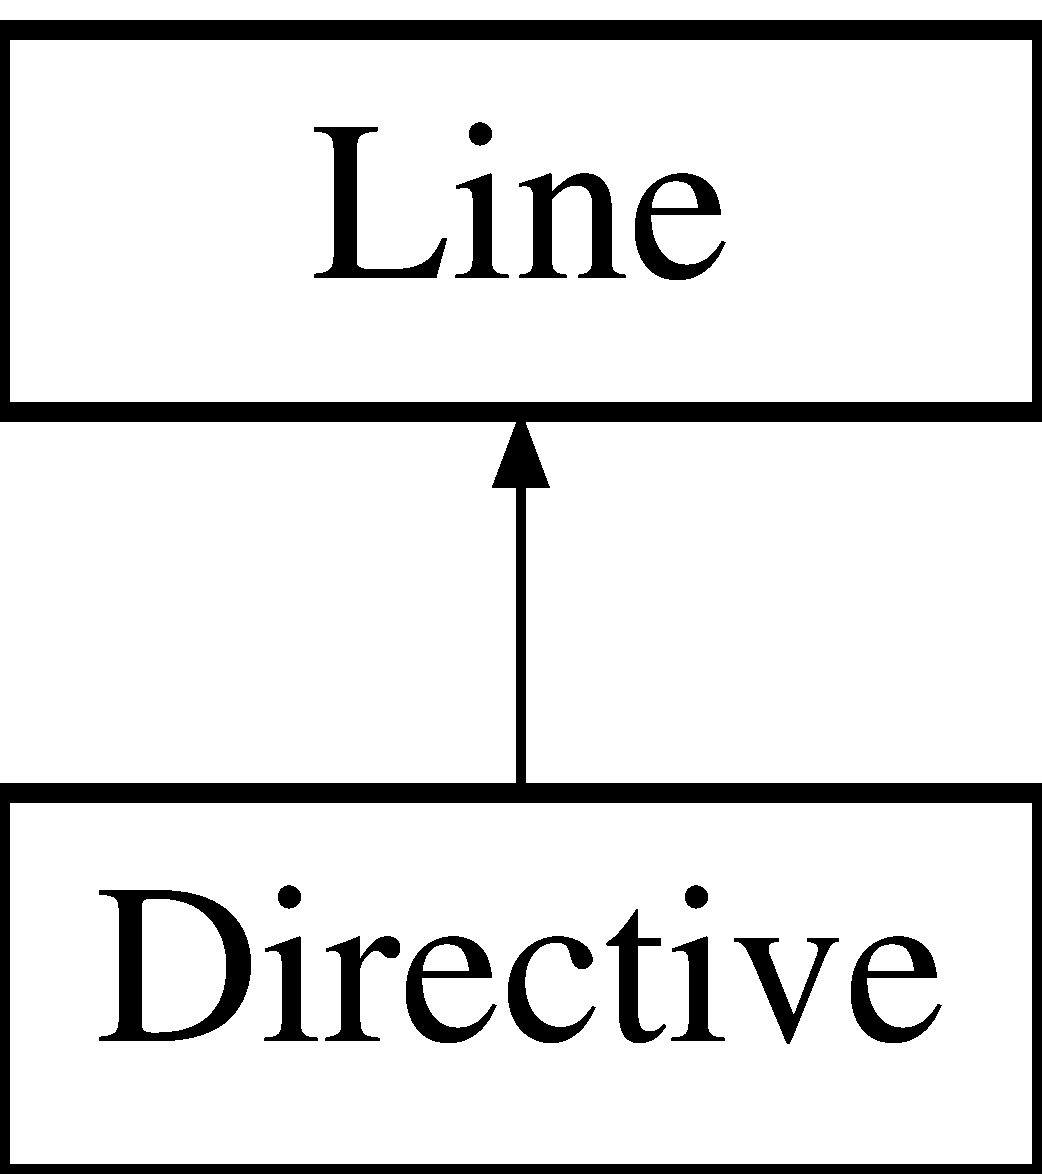
\includegraphics[height=2.000000cm]{class_directive}
\end{center}
\end{figure}
\subsection*{Public Member Functions}
\begin{DoxyCompactItemize}
\item 
\hypertarget{class_directive_a7487120f679e1b4d01843ad6feac7e07}{}\hyperlink{class_directive_a7487120f679e1b4d01843ad6feac7e07}{Directive} (string)\label{class_directive_a7487120f679e1b4d01843ad6feac7e07}

\begin{DoxyCompactList}\small\item\em Constructor of the \hyperlink{class_directive}{Directive}. \end{DoxyCompactList}\item 
\hypertarget{class_directive_ac2f912e3997d9fed8bc289d77fc06305}{}\hyperlink{class_directive_ac2f912e3997d9fed8bc289d77fc06305}{Directive} (string, string)\label{class_directive_ac2f912e3997d9fed8bc289d77fc06305}

\begin{DoxyCompactList}\small\item\em Constructor of the \hyperlink{class_directive}{Directive} with directive, content and an boolean. \end{DoxyCompactList}\item 
\hypertarget{class_directive_adbe3bd8e72354bde2b7d809348d0d527}{}\hyperlink{class_directive_adbe3bd8e72354bde2b7d809348d0d527}{Directive} (string, string, bool)\label{class_directive_adbe3bd8e72354bde2b7d809348d0d527}

\begin{DoxyCompactList}\small\item\em Constructor of the \hyperlink{class_directive}{Directive} with directive, content and an boolean. \end{DoxyCompactList}\item 
\hypertarget{class_directive_aa9a48f09b0472c835ffa366bcff74f51}{}virtual \hyperlink{class_directive_aa9a48f09b0472c835ffa366bcff74f51}{$\sim$\+Directive} ()\label{class_directive_aa9a48f09b0472c835ffa366bcff74f51}

\begin{DoxyCompactList}\small\item\em Destructor of the \hyperlink{class_directive}{Directive}. \end{DoxyCompactList}\item 
\hypertarget{class_directive_a0d574b0ffc25eb1fbc49032534e7ff44}{}virtual t\+\_\+\+Line \hyperlink{class_directive_a0d574b0ffc25eb1fbc49032534e7ff44}{type\+\_\+line} ()\label{class_directive_a0d574b0ffc25eb1fbc49032534e7ff44}

\begin{DoxyCompactList}\small\item\em get the type of the line \end{DoxyCompactList}\item 
\hypertarget{class_directive_a2fd56d5580ad7a993782649d7867732f}{}virtual string \hyperlink{class_directive_a2fd56d5580ad7a993782649d7867732f}{to\+\_\+string} ()\label{class_directive_a2fd56d5580ad7a993782649d7867732f}

\begin{DoxyCompactList}\small\item\em get the string of the \hyperlink{class_directive}{Directive} \end{DoxyCompactList}\item 
\hypertarget{class_directive_aaeb0e95f88f41425718859daeb2116ad}{}virtual string \hyperlink{class_directive_aaeb0e95f88f41425718859daeb2116ad}{get\+\_\+content} ()\label{class_directive_aaeb0e95f88f41425718859daeb2116ad}

\begin{DoxyCompactList}\small\item\em get the string of the \hyperlink{class_directive}{Directive} \end{DoxyCompactList}\item 
\hypertarget{class_directive_a59b72d2ebc140e3ac0a0d6d789bb5bba}{}virtual void \hyperlink{class_directive_a59b72d2ebc140e3ac0a0d6d789bb5bba}{set\+\_\+content} (string)\label{class_directive_a59b72d2ebc140e3ac0a0d6d789bb5bba}

\begin{DoxyCompactList}\small\item\em set the string of the \hyperlink{class_directive}{Directive} \end{DoxyCompactList}\item 
\hypertarget{class_directive_ae585a212960cc755c057f85533ddc71e}{}bool \hyperlink{class_directive_ae585a212960cc755c057f85533ddc71e}{is\+\_\+function} ()\label{class_directive_ae585a212960cc755c057f85533ddc71e}

\begin{DoxyCompactList}\small\item\em return true if the directive indicate a function \end{DoxyCompactList}\item 
\hypertarget{class_directive_a5c3ac59a9d3bc3c16341124482370843}{}virtual t\+\_\+\+Inst \hyperlink{class_directive_a5c3ac59a9d3bc3c16341124482370843}{get\+\_\+type} ()\label{class_directive_a5c3ac59a9d3bc3c16341124482370843}

\begin{DoxyCompactList}\small\item\em return the type of the instruction \end{DoxyCompactList}\end{DoxyCompactItemize}
\subsection*{Public Attributes}
\begin{DoxyCompactItemize}
\item 
\hypertarget{class_directive_a3e89203d14d83c6ff8da7a1c49b9a60e}{}string {\bfseries \+\_\+dir}\label{class_directive_a3e89203d14d83c6ff8da7a1c49b9a60e}

\item 
\hypertarget{class_directive_aaeaa71135c6d434d58db763a1e2b70e3}{}string {\bfseries \+\_\+value}\label{class_directive_aaeaa71135c6d434d58db763a1e2b70e3}

\item 
\hypertarget{class_directive_ae9e02b1ecc6a1b5387f5227959984c1f}{}bool {\bfseries \+\_\+isfunction}\label{class_directive_ae9e02b1ecc6a1b5387f5227959984c1f}

\end{DoxyCompactItemize}
\subsection*{Additional Inherited Members}


\subsection{Detailed Description}
class representing an \hyperlink{class_directive}{Directive} herited by \hyperlink{class_line}{Line} 

The documentation for this class was generated from the following file\+:\begin{DoxyCompactItemize}
\item 
\hyperlink{_directive_8h}{Directive.\+h}\end{DoxyCompactItemize}

\hypertarget{class_function}{}\section{Function Class Reference}
\label{class_function}\index{Function@{Function}}


class representing a \hyperlink{class_function}{Function} on a program  




{\ttfamily \#include $<$Function.\+h$>$}

\subsection*{Public Member Functions}
\begin{DoxyCompactItemize}
\item 
\hypertarget{class_function_ae206568fd4fd4c885e3ccff76345c4e6}{}\hyperlink{class_function_ae206568fd4fd4c885e3ccff76345c4e6}{Function} ()\label{class_function_ae206568fd4fd4c885e3ccff76345c4e6}

\begin{DoxyCompactList}\small\item\em Constructor of a function. \end{DoxyCompactList}\item 
\hypertarget{class_function_a3b03f7cf0b75d16edebdda1dee1db6fd}{}\hyperlink{class_function_a3b03f7cf0b75d16edebdda1dee1db6fd}{$\sim$\+Function} ()\label{class_function_a3b03f7cf0b75d16edebdda1dee1db6fd}

\begin{DoxyCompactList}\small\item\em Destructor of a function. \end{DoxyCompactList}\item 
\hypertarget{class_function_a67ffa7175c8ab513df6db299b877ad97}{}void \hyperlink{class_function_a67ffa7175c8ab513df6db299b877ad97}{set\+\_\+head} (\hyperlink{class_line}{Line} $\ast$)\label{class_function_a67ffa7175c8ab513df6db299b877ad97}

\begin{DoxyCompactList}\small\item\em setter of the head of the function \end{DoxyCompactList}\item 
\hypertarget{class_function_af5b88d118098c4cd6e5e3a4d324b8b48}{}void \hyperlink{class_function_af5b88d118098c4cd6e5e3a4d324b8b48}{set\+\_\+end} (\hyperlink{class_line}{Line} $\ast$)\label{class_function_af5b88d118098c4cd6e5e3a4d324b8b48}

\begin{DoxyCompactList}\small\item\em setter of the end of the function \end{DoxyCompactList}\item 
\hypertarget{class_function_a1ca74e7cd3f2681ae8ddcc70241fdc29}{}\hyperlink{class_line}{Line} $\ast$ \hyperlink{class_function_a1ca74e7cd3f2681ae8ddcc70241fdc29}{get\+\_\+head} ()\label{class_function_a1ca74e7cd3f2681ae8ddcc70241fdc29}

\begin{DoxyCompactList}\small\item\em get the head of the function \end{DoxyCompactList}\item 
\hypertarget{class_function_a6789e258845ec7b9d2fd922c6291396d}{}\hyperlink{class_basic__block}{Basic\+\_\+block} $\ast$ {\bfseries get\+\_\+first\+B\+B} ()\label{class_function_a6789e258845ec7b9d2fd922c6291396d}

\item 
\hypertarget{class_function_a319af56932faa6253ebe9db1c821eb4d}{}\hyperlink{class_line}{Line} $\ast$ \hyperlink{class_function_a319af56932faa6253ebe9db1c821eb4d}{get\+\_\+end} ()\label{class_function_a319af56932faa6253ebe9db1c821eb4d}

\begin{DoxyCompactList}\small\item\em get the ending \hyperlink{class_line}{Line} of the function \end{DoxyCompactList}\item 
\hypertarget{class_function_ade8a6050da83010be473a6581d65a3ce}{}void \hyperlink{class_function_ade8a6050da83010be473a6581d65a3ce}{display} ()\label{class_function_ade8a6050da83010be473a6581d65a3ce}

\begin{DoxyCompactList}\small\item\em display the function \end{DoxyCompactList}\item 
\hypertarget{class_function_a0b62379b4e18c9440963b54d2e8991b0}{}int \hyperlink{class_function_a0b62379b4e18c9440963b54d2e8991b0}{size} ()\label{class_function_a0b62379b4e18c9440963b54d2e8991b0}

\begin{DoxyCompactList}\small\item\em get number of Lines of the function \end{DoxyCompactList}\item 
\hypertarget{class_function_acd08be840c48abd3c0c0c20ca4b5192a}{}void \hyperlink{class_function_acd08be840c48abd3c0c0c20ca4b5192a}{restitution} (string const)\label{class_function_acd08be840c48abd3c0c0c20ca4b5192a}

\begin{DoxyCompactList}\small\item\em restitute the function in a file \end{DoxyCompactList}\item 
\hypertarget{class_function_a5b1550f534becc9b7ae9fe679fc8db10}{}void \hyperlink{class_function_a5b1550f534becc9b7ae9fe679fc8db10}{add\+\_\+\+B\+B} (\hyperlink{class_line}{Line} $\ast$, \hyperlink{class_line}{Line} $\ast$, \hyperlink{class_line}{Line} $\ast$, int)\label{class_function_a5b1550f534becc9b7ae9fe679fc8db10}

\begin{DoxyCompactList}\small\item\em creates a new B\+B with the given start line, end line and branch line and its index, add it to the B\+B list of this \end{DoxyCompactList}\item 
\hypertarget{class_function_a6094f123294ccbb891fa4145fd5b1b0a}{}void \hyperlink{class_function_a6094f123294ccbb891fa4145fd5b1b0a}{comput\+\_\+basic\+\_\+block} ()\label{class_function_a6094f123294ccbb891fa4145fd5b1b0a}

\begin{DoxyCompactList}\small\item\em Calculate the basics bolck of the function. \end{DoxyCompactList}\item 
\hypertarget{class_function_a4ddde4ac1ff488dfcbfcaee71f727a48}{}int \hyperlink{class_function_a4ddde4ac1ff488dfcbfcaee71f727a48}{nbr\+\_\+\+B\+B} ()\label{class_function_a4ddde4ac1ff488dfcbfcaee71f727a48}

\begin{DoxyCompactList}\small\item\em get the number of Basic block in the function \end{DoxyCompactList}\item 
\hypertarget{class_function_ae11968b8ca5497526e9448b67823d373}{}\hyperlink{class_basic__block}{Basic\+\_\+block} $\ast$ \hyperlink{class_function_ae11968b8ca5497526e9448b67823d373}{get\+\_\+\+B\+B} (int)\label{class_function_ae11968b8ca5497526e9448b67823d373}

\begin{DoxyCompactList}\small\item\em get the Basic Block at a position in the B\+B list \end{DoxyCompactList}\item 
\hypertarget{class_function_a18797dfd75ba34acf0e73b69da8311ec}{}list$<$ \hyperlink{class_basic__block}{Basic\+\_\+block} $\ast$ $>$\+::iterator \hyperlink{class_function_a18797dfd75ba34acf0e73b69da8311ec}{bb\+\_\+list\+\_\+begin} ()\label{class_function_a18797dfd75ba34acf0e73b69da8311ec}

\begin{DoxyCompactList}\small\item\em iterators of the B\+B list \end{DoxyCompactList}\item 
\hypertarget{class_function_a06be1b0a730b4ead3da6bb5529df9788}{}list$<$ \hyperlink{class_basic__block}{Basic\+\_\+block} $\ast$ $>$\+::iterator {\bfseries bb\+\_\+list\+\_\+end} ()\label{class_function_a06be1b0a730b4ead3da6bb5529df9788}

\item 
\hypertarget{class_function_a1c8830219ce4306c22a933b17f54cc6f}{}void \hyperlink{class_function_a1c8830219ce4306c22a933b17f54cc6f}{comput\+\_\+label} ()\label{class_function_a1c8830219ce4306c22a933b17f54cc6f}

\begin{DoxyCompactList}\small\item\em comput labels of the function in list \end{DoxyCompactList}\item 
\hypertarget{class_function_a4b2e9837c4b506b3c7a6d1488d9914d1}{}\hyperlink{class_label}{Label} $\ast$ \hyperlink{class_function_a4b2e9837c4b506b3c7a6d1488d9914d1}{get\+\_\+label} (int)\label{class_function_a4b2e9837c4b506b3c7a6d1488d9914d1}

\begin{DoxyCompactList}\small\item\em get a specific label of the function \end{DoxyCompactList}\item 
\hypertarget{class_function_a3f3807e12e695ffe23e1ef44edcd262b}{}int \hyperlink{class_function_a3f3807e12e695ffe23e1ef44edcd262b}{nbr\+\_\+label} ()\label{class_function_a3f3807e12e695ffe23e1ef44edcd262b}

\begin{DoxyCompactList}\small\item\em get the size of the list label \end{DoxyCompactList}\item 
\hypertarget{class_function_ae55c0232d0eced8830daf57293229db8}{}\hyperlink{class_basic__block}{Basic\+\_\+block} $\ast$ \hyperlink{class_function_ae55c0232d0eced8830daf57293229db8}{find\+\_\+label\+\_\+\+B\+B} (\hyperlink{class_o_p_label}{O\+P\+Label} $\ast$)\label{class_function_ae55c0232d0eced8830daf57293229db8}

\begin{DoxyCompactList}\small\item\em Get the basic block that starts with a given label (operand) \end{DoxyCompactList}\item 
\hypertarget{class_function_a3c52c8cb82e0137f02771331018b655c}{}void \hyperlink{class_function_a3c52c8cb82e0137f02771331018b655c}{comput\+\_\+succ\+\_\+pred\+\_\+\+B\+B} ()\label{class_function_a3c52c8cb82e0137f02771331018b655c}

\begin{DoxyCompactList}\small\item\em Computes the successors and predecessors of each Basic block. \end{DoxyCompactList}\item 
\hypertarget{class_function_aaa0d06640a5075c416106a88bd9a833a}{}void \hyperlink{class_function_aaa0d06640a5075c416106a88bd9a833a}{test} ()\label{class_function_aaa0d06640a5075c416106a88bd9a833a}

\begin{DoxyCompactList}\small\item\em method to perform some test, usefull for testing methods on basic blocks \end{DoxyCompactList}\item 
\hypertarget{class_function_a21b614fb69692ba00240831c8fe8beb9}{}void \hyperlink{class_function_a21b614fb69692ba00240831c8fe8beb9}{compute\+\_\+live\+\_\+var} ()\label{class_function_a21b614fb69692ba00240831c8fe8beb9}

\begin{DoxyCompactList}\small\item\em computes live variable for each basic blocks \end{DoxyCompactList}\item 
\hypertarget{class_function_a9ecf8e774164937c3dfdb989ebe1c866}{}void \hyperlink{class_function_a9ecf8e774164937c3dfdb989ebe1c866}{compute\+\_\+dom} ()\label{class_function_a9ecf8e774164937c3dfdb989ebe1c866}

\begin{DoxyCompactList}\small\item\em computes dominators for each basic blocks \end{DoxyCompactList}\end{DoxyCompactItemize}


\subsection{Detailed Description}
class representing a \hyperlink{class_function}{Function} on a program 

The documentation for this class was generated from the following file\+:\begin{DoxyCompactItemize}
\item 
\hyperlink{_function_8h}{Function.\+h}\end{DoxyCompactItemize}

\hypertarget{class_instruction}{}\section{Instruction Class Reference}
\label{class_instruction}\index{Instruction@{Instruction}}


class representing an instruction which herited by \hyperlink{class_line}{Line}  




{\ttfamily \#include $<$Instruction.\+h$>$}

Inheritance diagram for Instruction\+:\begin{figure}[H]
\begin{center}
\leavevmode
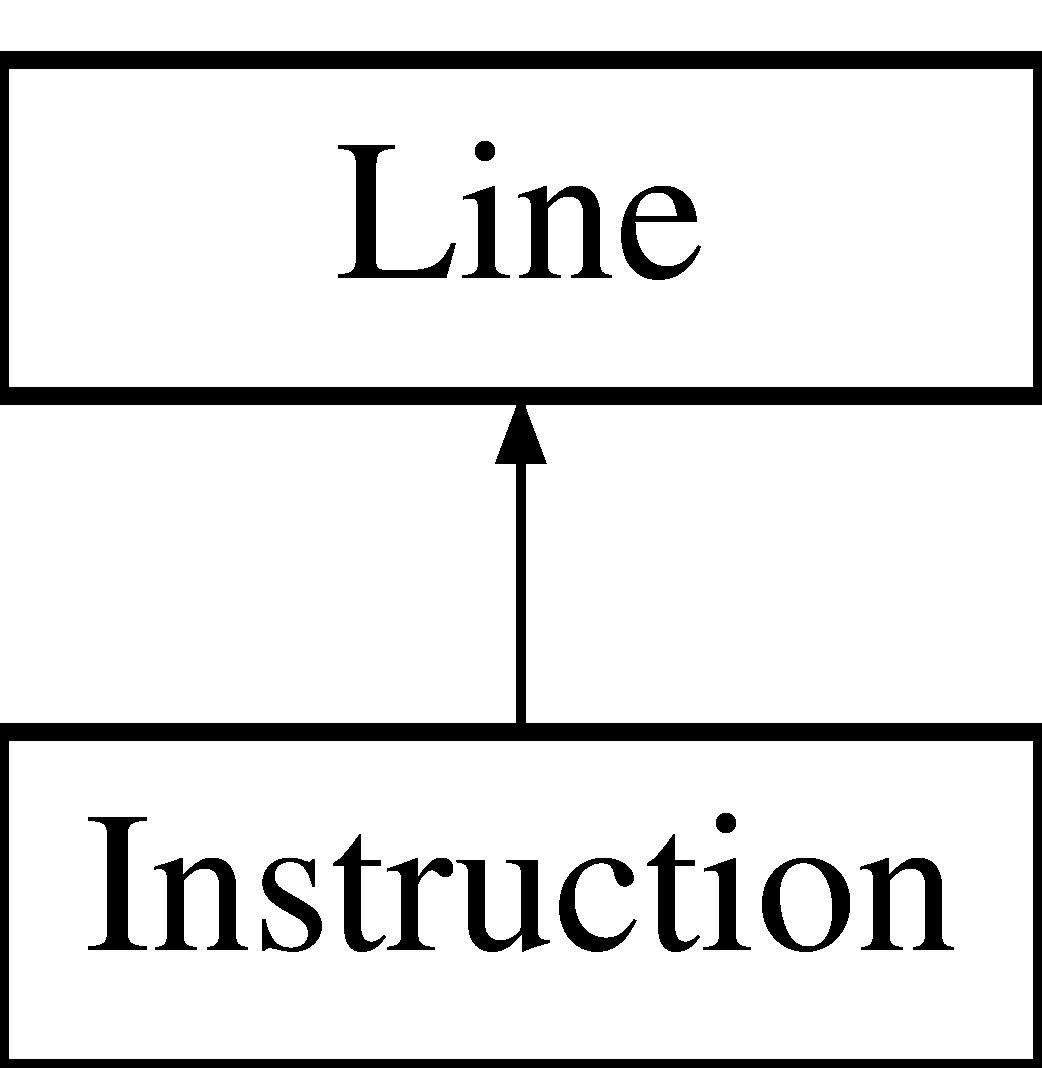
\includegraphics[height=2.000000cm]{class_instruction}
\end{center}
\end{figure}
\subsection*{Public Member Functions}
\begin{DoxyCompactItemize}
\item 
\hyperlink{class_instruction_a055c483afc0512b68f6211fdbb6774ba}{Instruction} (string, t\+\_\+\+Operator, t\+\_\+\+Inst, \hyperlink{class_operand}{Operand} $\ast$, \hyperlink{class_operand}{Operand} $\ast$, \hyperlink{class_operand}{Operand} $\ast$)
\begin{DoxyCompactList}\small\item\em get the Opcode value accessor of the opcode \end{DoxyCompactList}\item 
\hypertarget{class_instruction_a2f1ed1606d4090b8a4c255e3af9e34c8}{}\hyperlink{class_instruction_a2f1ed1606d4090b8a4c255e3af9e34c8}{Instruction} (t\+\_\+\+Operator, \hyperlink{class_operand}{Operand} $\ast$, \hyperlink{class_operand}{Operand} $\ast$, \hyperlink{class_operand}{Operand} $\ast$)\label{class_instruction_a2f1ed1606d4090b8a4c255e3af9e34c8}

\begin{DoxyCompactList}\small\item\em Constructor with 3 Operands of the class instruction. \end{DoxyCompactList}\item 
\hypertarget{class_instruction_a0b1ed4432c9c5823ee9e522c7d11bb5f}{}\hyperlink{class_instruction_a0b1ed4432c9c5823ee9e522c7d11bb5f}{Instruction} (t\+\_\+\+Operator, \hyperlink{class_operand}{Operand} $\ast$, \hyperlink{class_operand}{Operand} $\ast$)\label{class_instruction_a0b1ed4432c9c5823ee9e522c7d11bb5f}

\begin{DoxyCompactList}\small\item\em Constructor with 2 Operands of the class instruction. \end{DoxyCompactList}\item 
\hypertarget{class_instruction_a6ae2a4dd83500f9d538a653823161b1c}{}\hyperlink{class_instruction_a6ae2a4dd83500f9d538a653823161b1c}{Instruction} (t\+\_\+\+Operator, \hyperlink{class_operand}{Operand} $\ast$)\label{class_instruction_a6ae2a4dd83500f9d538a653823161b1c}

\begin{DoxyCompactList}\small\item\em Constructor with 1 \hyperlink{class_operand}{Operand} of the class instruction. \end{DoxyCompactList}\item 
\hypertarget{class_instruction_ab2d989cc18e9bf0eeee194a7614514fa}{}\hyperlink{class_instruction_ab2d989cc18e9bf0eeee194a7614514fa}{Instruction} (t\+\_\+\+Operator)\label{class_instruction_ab2d989cc18e9bf0eeee194a7614514fa}

\begin{DoxyCompactList}\small\item\em Constructor without Operands of the class instruction. \end{DoxyCompactList}\item 
\hypertarget{class_instruction_a3f1031e811b710787678f8faf8cc9672}{}virtual \hyperlink{class_instruction_a3f1031e811b710787678f8faf8cc9672}{$\sim$\+Instruction} ()\label{class_instruction_a3f1031e811b710787678f8faf8cc9672}

\begin{DoxyCompactList}\small\item\em Destructor of the class instruction. \end{DoxyCompactList}\item 
\hypertarget{class_instruction_aab8e6a16b8bab5ca90b554086cc3c825}{}bool \hyperlink{class_instruction_aab8e6a16b8bab5ca90b554086cc3c825}{is\+\_\+branch} ()\label{class_instruction_aab8e6a16b8bab5ca90b554086cc3c825}

\begin{DoxyCompactList}\small\item\em test if the instruction is a branch \end{DoxyCompactList}\item 
\hypertarget{class_instruction_ab2a6352a09271a588f6930852a361f67}{}bool \hyperlink{class_instruction_ab2a6352a09271a588f6930852a361f67}{is\+\_\+call} ()\label{class_instruction_ab2a6352a09271a588f6930852a361f67}

\begin{DoxyCompactList}\small\item\em test if the instruction is a call \end{DoxyCompactList}\item 
\hypertarget{class_instruction_a1b607074554bc160142786c125bde530}{}bool \hyperlink{class_instruction_a1b607074554bc160142786c125bde530}{is\+\_\+cond\+\_\+branch} ()\label{class_instruction_a1b607074554bc160142786c125bde530}

\begin{DoxyCompactList}\small\item\em test if the instruction is a conditionnal branch \end{DoxyCompactList}\item 
\hypertarget{class_instruction_affdf2382cd36277fb4427cd3b07c1402}{}bool \hyperlink{class_instruction_affdf2382cd36277fb4427cd3b07c1402}{is\+\_\+indirect\+\_\+branch} ()\label{class_instruction_affdf2382cd36277fb4427cd3b07c1402}

\begin{DoxyCompactList}\small\item\em test if the instruction a branch and the target adress is in a register \end{DoxyCompactList}\item 
\hypertarget{class_instruction_a2222ad40481088c12a38c5f340bcd86b}{}bool \hyperlink{class_instruction_a2222ad40481088c12a38c5f340bcd86b}{is\+\_\+nop} ()\label{class_instruction_a2222ad40481088c12a38c5f340bcd86b}

\begin{DoxyCompactList}\small\item\em test if the instruction a branch and the target adress is in a register \end{DoxyCompactList}\item 
\hypertarget{class_instruction_a1c79865faf9baa4d70edf81e956d952d}{}bool \hyperlink{class_instruction_a1c79865faf9baa4d70edf81e956d952d}{is\+\_\+mem} ()\label{class_instruction_a1c79865faf9baa4d70edf81e956d952d}

\begin{DoxyCompactList}\small\item\em test if the instruction is a memory access \end{DoxyCompactList}\item 
\hypertarget{class_instruction_aee32f4bb91480afc74375beb139af4d6}{}bool \hyperlink{class_instruction_aee32f4bb91480afc74375beb139af4d6}{is\+\_\+mem\+\_\+load} ()\label{class_instruction_aee32f4bb91480afc74375beb139af4d6}

\begin{DoxyCompactList}\small\item\em test if the instruction is a memory access that reads a value \end{DoxyCompactList}\item 
\hypertarget{class_instruction_a4455144397d239eb61bcfa2b0e16bf67}{}bool \hyperlink{class_instruction_a4455144397d239eb61bcfa2b0e16bf67}{is\+\_\+mem\+\_\+store} ()\label{class_instruction_a4455144397d239eb61bcfa2b0e16bf67}

\begin{DoxyCompactList}\small\item\em test if the instruction is a memory access that writes a value \end{DoxyCompactList}\item 
bool \hyperlink{class_instruction_ae5d54f535adab416c53eb0ff6a438804}{is\+\_\+dep\+\_\+\+R\+A\+W1} (\hyperlink{class_instruction}{Instruction} $\ast$i2)
\begin{DoxyCompactList}\small\item\em return if there is dependance R\+A\+W between the current instruction and the first source operand of i2 \end{DoxyCompactList}\item 
bool \hyperlink{class_instruction_aa28ae5f427ee02c96466f1ac68060f87}{is\+\_\+dep\+\_\+\+R\+A\+W2} (\hyperlink{class_instruction}{Instruction} $\ast$i2)
\begin{DoxyCompactList}\small\item\em return if there is dependance R\+A\+W between the current instruction and the second source operand of i2 \end{DoxyCompactList}\item 
bool \hyperlink{class_instruction_a36c0faedd74af14b403ba7063af5d07f}{is\+\_\+dep\+\_\+\+W\+A\+R1} (\hyperlink{class_instruction}{Instruction} $\ast$i2)
\begin{DoxyCompactList}\small\item\em test if there is dependance W\+A\+R between the first source operande of the current instruction if any and the destination register operande i2 if any \end{DoxyCompactList}\item 
bool \hyperlink{class_instruction_a04471df677984f67ec13de88f55e3703}{is\+\_\+dep\+\_\+\+W\+A\+R2} (\hyperlink{class_instruction}{Instruction} $\ast$i2)
\begin{DoxyCompactList}\small\item\em test if there is dependance W\+A\+R between the second source operande of the current instruction if any and the destination register operande i2 if any \end{DoxyCompactList}\item 
\hypertarget{class_instruction_adb43e7019987daebb3970335aba695cc}{}\hyperlink{class_o_p_register}{O\+P\+Register} $\ast$ \hyperlink{class_instruction_adb43e7019987daebb3970335aba695cc}{get\+\_\+reg\+\_\+dst} ()\label{class_instruction_adb43e7019987daebb3970335aba695cc}

\begin{DoxyCompactList}\small\item\em get the register destination of the instruction, if any \end{DoxyCompactList}\item 
\hypertarget{class_instruction_ac353a6ad2b3f3b1aee179d5910b5127b}{}\hyperlink{class_o_p_register}{O\+P\+Register} $\ast$ \hyperlink{class_instruction_ac353a6ad2b3f3b1aee179d5910b5127b}{get\+\_\+reg\+\_\+src1} ()\label{class_instruction_ac353a6ad2b3f3b1aee179d5910b5127b}

\begin{DoxyCompactList}\small\item\em get the first register source of the instruction \end{DoxyCompactList}\item 
\hypertarget{class_instruction_a0eb007b1b0a038610e71a58af3bb6438}{}\hyperlink{class_o_p_register}{O\+P\+Register} $\ast$ \hyperlink{class_instruction_a0eb007b1b0a038610e71a58af3bb6438}{get\+\_\+reg\+\_\+src2} ()\label{class_instruction_a0eb007b1b0a038610e71a58af3bb6438}

\begin{DoxyCompactList}\small\item\em get the second register source of the instruction \end{DoxyCompactList}\item 
\hypertarget{class_instruction_aa32973fb1e9e24659095e4795c153c8a}{}\hyperlink{class_o_p_label}{O\+P\+Label} $\ast$ \hyperlink{class_instruction_aa32973fb1e9e24659095e4795c153c8a}{get\+\_\+op\+\_\+label} ()\label{class_instruction_aa32973fb1e9e24659095e4795c153c8a}

\begin{DoxyCompactList}\small\item\em get the label operand of the instruction, if any \end{DoxyCompactList}\item 
\hypertarget{class_instruction_a1195d03eb4ff6024b20cd2cec1c8a1e0}{}t\+\_\+\+Operator {\bfseries get\+\_\+opcode} ()\label{class_instruction_a1195d03eb4ff6024b20cd2cec1c8a1e0}

\item 
\hypertarget{class_instruction_aeba180e03a3ac7f7ecba7635d454566f}{}string \hyperlink{class_instruction_aeba180e03a3ac7f7ecba7635d454566f}{string\+\_\+opcode} ()\label{class_instruction_aeba180e03a3ac7f7ecba7635d454566f}

\begin{DoxyCompactList}\small\item\em get the string Opcode value accessor of the string opcode \end{DoxyCompactList}\item 
\hypertarget{class_instruction_a49524f35c4ade25c663d798e3a5df2cb}{}void \hyperlink{class_instruction_a49524f35c4ade25c663d798e3a5df2cb}{set\+\_\+opcode} (t\+\_\+\+Operator newop)\label{class_instruction_a49524f35c4ade25c663d798e3a5df2cb}

\begin{DoxyCompactList}\small\item\em set the opcode value setter of the opcode \end{DoxyCompactList}\item 
\hypertarget{class_instruction_a86e8d9627ad78884d75481693a6196ef}{}t\+\_\+\+Format \hyperlink{class_instruction_a86e8d9627ad78884d75481693a6196ef}{get\+\_\+format} ()\label{class_instruction_a86e8d9627ad78884d75481693a6196ef}

\begin{DoxyCompactList}\small\item\em get the format of the \hyperlink{class_instruction}{Instruction} accessor of the format (see \hyperlink{_enum__type_8h_source}{Enum\+\_\+type.\+h}) \end{DoxyCompactList}\item 
\hypertarget{class_instruction_ae619398c5531b1f2042fb4caa893cdee}{}virtual t\+\_\+\+Inst \hyperlink{class_instruction_ae619398c5531b1f2042fb4caa893cdee}{get\+\_\+type} ()\label{class_instruction_ae619398c5531b1f2042fb4caa893cdee}

\begin{DoxyCompactList}\small\item\em get the Type of the \hyperlink{class_instruction}{Instruction} accessor of the Type (see \hyperlink{_enum__type_8h_source}{Enum\+\_\+type.\+h}) \end{DoxyCompactList}\item 
\hypertarget{class_instruction_adcab5ded0016e613826be14514abbcc8}{}virtual t\+\_\+\+Line \hyperlink{class_instruction_adcab5ded0016e613826be14514abbcc8}{type\+\_\+line} ()\label{class_instruction_adcab5ded0016e613826be14514abbcc8}

\begin{DoxyCompactList}\small\item\em get the type of the line \end{DoxyCompactList}\item 
\hypertarget{class_instruction_aed87de5e9259f4f15dc885425528f1fe}{}virtual string \hyperlink{class_instruction_aed87de5e9259f4f15dc885425528f1fe}{to\+\_\+string} ()\label{class_instruction_aed87de5e9259f4f15dc885425528f1fe}

\begin{DoxyCompactList}\small\item\em get the name string instruction \end{DoxyCompactList}\item 
\hypertarget{class_instruction_a5b258bf1dfb9f6fa2fff0af0e7c211d8}{}virtual string \hyperlink{class_instruction_a5b258bf1dfb9f6fa2fff0af0e7c211d8}{get\+\_\+content} ()\label{class_instruction_a5b258bf1dfb9f6fa2fff0af0e7c211d8}

\begin{DoxyCompactList}\small\item\em get the string of the instruction \end{DoxyCompactList}\item 
\hypertarget{class_instruction_aec1a1ab575287b532fb8d43cfa364e30}{}virtual void \hyperlink{class_instruction_aec1a1ab575287b532fb8d43cfa364e30}{set\+\_\+content} (string)\label{class_instruction_aec1a1ab575287b532fb8d43cfa364e30}

\begin{DoxyCompactList}\small\item\em set the string of the instruction \end{DoxyCompactList}\item 
\hypertarget{class_instruction_a2d2d966c6269e1e0dbfbeb8aabafeeb4}{}string \hyperlink{class_instruction_a2d2d966c6269e1e0dbfbeb8aabafeeb4}{string\+\_\+form} ()\label{class_instruction_a2d2d966c6269e1e0dbfbeb8aabafeeb4}

\begin{DoxyCompactList}\small\item\em set the string format \end{DoxyCompactList}\item 
\hypertarget{class_instruction_ac2d81dcf8ddd82e31262c7adb1a0df69}{}string \hyperlink{class_instruction_ac2d81dcf8ddd82e31262c7adb1a0df69}{string\+\_\+type} ()\label{class_instruction_ac2d81dcf8ddd82e31262c7adb1a0df69}

\begin{DoxyCompactList}\small\item\em set the string Type of instruction \end{DoxyCompactList}\item 
\hypertarget{class_instruction_a14c5f91c242a5b58eda9f123ad331cbe}{}int \hyperlink{class_instruction_a14c5f91c242a5b58eda9f123ad331cbe}{get\+\_\+index} ()\label{class_instruction_a14c5f91c242a5b58eda9f123ad331cbe}

\begin{DoxyCompactList}\small\item\em get the index of instruction \end{DoxyCompactList}\item 
\hypertarget{class_instruction_af1608cfea660c46e8a8b4bbac948406a}{}void \hyperlink{class_instruction_af1608cfea660c46e8a8b4bbac948406a}{set\+\_\+index} (int)\label{class_instruction_af1608cfea660c46e8a8b4bbac948406a}

\begin{DoxyCompactList}\small\item\em set the index of instruction \end{DoxyCompactList}\item 
t\+\_\+\+Dep \hyperlink{class_instruction_ac8d86b800140a08cb03d82f83f363fa4}{is\+\_\+dependant} (\hyperlink{class_instruction}{Instruction} $\ast$i2)
\begin{DoxyCompactList}\small\item\em get the dependance between the current instruction and i2 \end{DoxyCompactList}\item 
bool \hyperlink{class_instruction_a4c902c5a8fdc8c8841ec24f389605fd5}{is\+\_\+dep\+\_\+\+R\+A\+W} (\hyperlink{class_instruction}{Instruction} $\ast$i2)
\begin{DoxyCompactList}\small\item\em get the information if there is dependance R\+A\+W between the current instruction and i2 \end{DoxyCompactList}\item 
bool \hyperlink{class_instruction_ae79b239c6ab30a15064b5a00944ad65a}{is\+\_\+dep\+\_\+\+W\+A\+R} (\hyperlink{class_instruction}{Instruction} $\ast$i2)
\begin{DoxyCompactList}\small\item\em get the information if there is dependance W\+A\+R between the current instruction and i2 \end{DoxyCompactList}\item 
bool \hyperlink{class_instruction_a30c159faa5c462bb2c7ae7562c9c8254}{is\+\_\+dep\+\_\+\+W\+A\+W} (\hyperlink{class_instruction}{Instruction} $\ast$i2)
\begin{DoxyCompactList}\small\item\em get the information if there is dependance W\+A\+W between the current instruction and i2 \end{DoxyCompactList}\item 
bool \hyperlink{class_instruction_a28526bda91b964d7fd81f85cee02c624}{is\+\_\+dep\+\_\+\+M\+E\+M} (\hyperlink{class_instruction}{Instruction} $\ast$i2)
\begin{DoxyCompactList}\small\item\em test if there is dependance M\+E\+M\+D\+E\+P between the current instruction and i2 \end{DoxyCompactList}\item 
int \hyperlink{class_instruction_a044a281355f25375a7765f24bdf614f3}{get\+\_\+nb\+Op} ()
\begin{DoxyCompactList}\small\item\em get the number of operand \end{DoxyCompactList}\item 
\hypertarget{class_instruction_a6ff2d531dffa43d3db22194459336d33}{}void \hyperlink{class_instruction_a6ff2d531dffa43d3db22194459336d33}{set\+\_\+number\+\_\+oper} (int)\label{class_instruction_a6ff2d531dffa43d3db22194459336d33}

\begin{DoxyCompactList}\small\item\em set the number of operand \end{DoxyCompactList}\item 
\hypertarget{class_instruction_ab8f6e21bc94df2198678a3cdbcfaa12e}{}void \hyperlink{class_instruction_ab8f6e21bc94df2198678a3cdbcfaa12e}{set\+\_\+link\+\_\+succ\+\_\+pred} (\hyperlink{class_instruction}{Instruction} $\ast$)\label{class_instruction_ab8f6e21bc94df2198678a3cdbcfaa12e}

\begin{DoxyCompactList}\small\item\em set the parameter as successor and this as predecessor of the parameter \end{DoxyCompactList}\item 
\hypertarget{class_instruction_a2fb436e52a0cc89e7ec08bf0e105bba3}{}void \hyperlink{class_instruction_a2fb436e52a0cc89e7ec08bf0e105bba3}{set\+\_\+next} (\hyperlink{class_instruction}{Instruction} $\ast$)\label{class_instruction_a2fb436e52a0cc89e7ec08bf0e105bba3}

\begin{DoxyCompactList}\small\item\em set the successor of the \hyperlink{class_instruction}{Instruction} \end{DoxyCompactList}\item 
\hypertarget{class_instruction_a93d5d6186afcf358c5a21f4c57a0d72e}{}\hyperlink{class_instruction}{Instruction} $\ast$ \hyperlink{class_instruction_a93d5d6186afcf358c5a21f4c57a0d72e}{get\+\_\+next} ()\label{class_instruction_a93d5d6186afcf358c5a21f4c57a0d72e}

\begin{DoxyCompactList}\small\item\em get the successor of the \hyperlink{class_instruction}{Instruction} (given by the schedule of instruction in its basic block) \end{DoxyCompactList}\item 
\hypertarget{class_instruction_a69d2992a0eb1fbe5fb6a38b52e13a804}{}void \hyperlink{class_instruction_a69d2992a0eb1fbe5fb6a38b52e13a804}{set\+\_\+prev} (\hyperlink{class_instruction}{Instruction} $\ast$)\label{class_instruction_a69d2992a0eb1fbe5fb6a38b52e13a804}

\begin{DoxyCompactList}\small\item\em setter of the predecessor of the \hyperlink{class_instruction}{Instruction} \end{DoxyCompactList}\item 
\hypertarget{class_instruction_afd6f27235469926b1e7979220495a6f0}{}\hyperlink{class_instruction}{Instruction} $\ast$ \hyperlink{class_instruction_afd6f27235469926b1e7979220495a6f0}{get\+\_\+prev} ()\label{class_instruction_afd6f27235469926b1e7979220495a6f0}

\begin{DoxyCompactList}\small\item\em get the predecessor of the \hyperlink{class_instruction}{Instruction} (given by the schedule of instruction in its basic block) \end{DoxyCompactList}\item 
\hypertarget{class_instruction_a3121dad231e2b4c27ac3cae6c8627ece}{}void \hyperlink{class_instruction_a3121dad231e2b4c27ac3cae6c8627ece}{add\+\_\+pred\+\_\+dep} (\hyperlink{structdep}{dep} $\ast$)\label{class_instruction_a3121dad231e2b4c27ac3cae6c8627ece}

\begin{DoxyCompactList}\small\item\em add a dependance with a predecessor instruction to the dependance type list \end{DoxyCompactList}\item 
\hypertarget{class_instruction_ab32531f8dd490b1c8396b6723f87bfae}{}\hyperlink{structdep}{dep} $\ast$ \hyperlink{class_instruction_ab32531f8dd490b1c8396b6723f87bfae}{get\+\_\+pred\+\_\+dep} (int i)\label{class_instruction_ab32531f8dd490b1c8396b6723f87bfae}

\begin{DoxyCompactList}\small\item\em get the dependance type with the ith predecessor instruction of the current instruction \end{DoxyCompactList}\item 
\hypertarget{class_instruction_acefc258dbcf45c19136dc86e47a82c0e}{}void \hyperlink{class_instruction_acefc258dbcf45c19136dc86e47a82c0e}{add\+\_\+succ\+\_\+dep} (\hyperlink{structdep}{dep} $\ast$)\label{class_instruction_acefc258dbcf45c19136dc86e47a82c0e}

\begin{DoxyCompactList}\small\item\em add a dependance with a successor to list of the dependance type of successors \end{DoxyCompactList}\item 
\hypertarget{class_instruction_a786e43bcd16d16a4db7c8a665c4d68af}{}void \hyperlink{class_instruction_a786e43bcd16d16a4db7c8a665c4d68af}{reset\+\_\+pred\+\_\+succ\+\_\+dep} ()\label{class_instruction_a786e43bcd16d16a4db7c8a665c4d68af}

\begin{DoxyCompactList}\small\item\em reset succ and pred dependances of this \end{DoxyCompactList}\item 
\hypertarget{class_instruction_a2c6f13ddda889e4e2b8b69897de6b733}{}list$<$ \hyperlink{structdep}{dep} $\ast$ $>$\+::iterator {\bfseries succ\+\_\+begin} ()\label{class_instruction_a2c6f13ddda889e4e2b8b69897de6b733}

\item 
\hypertarget{class_instruction_a0800ca0afbbc783b57170d981d406fb6}{}list$<$ \hyperlink{structdep}{dep} $\ast$ $>$\+::iterator {\bfseries succ\+\_\+end} ()\label{class_instruction_a0800ca0afbbc783b57170d981d406fb6}

\item 
\hypertarget{class_instruction_ad3bb47ea5f9e4b975e0191d6c96ffc30}{}\hyperlink{structdep}{dep} $\ast$ \hyperlink{class_instruction_ad3bb47ea5f9e4b975e0191d6c96ffc30}{get\+\_\+succ\+\_\+dep} (int i)\label{class_instruction_ad3bb47ea5f9e4b975e0191d6c96ffc30}

\begin{DoxyCompactList}\small\item\em get the ieme dependance type with successors from successor dependance type list of the current instruction \end{DoxyCompactList}\item 
\hypertarget{class_instruction_ab2d8c29efa78ec3c1a70f154a8c2f068}{}int \hyperlink{class_instruction_ab2d8c29efa78ec3c1a70f154a8c2f068}{get\+\_\+nb\+\_\+succ} ()\label{class_instruction_ab2d8c29efa78ec3c1a70f154a8c2f068}

\begin{DoxyCompactList}\small\item\em get the number of successor (dependance) of the \hyperlink{class_instruction}{Instruction} \end{DoxyCompactList}\item 
\hypertarget{class_instruction_a9e56e8e2c857abc409f27af9f80f9595}{}int \hyperlink{class_instruction_a9e56e8e2c857abc409f27af9f80f9595}{get\+\_\+nb\+\_\+pred} ()\label{class_instruction_a9e56e8e2c857abc409f27af9f80f9595}

\begin{DoxyCompactList}\small\item\em get the number of predecessor (dependance) of the \hyperlink{class_instruction}{Instruction} \end{DoxyCompactList}\item 
\hypertarget{class_instruction_ac2988d2fb858b720e009da03120ae4c7}{}int \hyperlink{class_instruction_ac2988d2fb858b720e009da03120ae4c7}{get\+\_\+latency} ()\label{class_instruction_ac2988d2fb858b720e009da03120ae4c7}

\begin{DoxyCompactList}\small\item\em return the latency of the instruction \end{DoxyCompactList}\item 
\hypertarget{class_instruction_af489e680ae3c69fd12b0a23e959172e5}{}void \hyperlink{class_instruction_af489e680ae3c69fd12b0a23e959172e5}{print\+\_\+succ\+\_\+dep} ()\label{class_instruction_af489e680ae3c69fd12b0a23e959172e5}

\begin{DoxyCompactList}\small\item\em print the dependance of this with instructions denoted by their index and the dependance type \end{DoxyCompactList}\end{DoxyCompactItemize}
\subsection*{Static Public Member Functions}
\begin{DoxyCompactItemize}
\item 
\hypertarget{class_instruction_ae309ff37d134500f75e1180182b02a6b}{}static bool {\bfseries is\+\_\+writed\+\_\+between} (int dst, \hyperlink{class_instruction}{Instruction} $\ast$i1, \hyperlink{class_instruction}{Instruction} $\ast$i2exclu)\label{class_instruction_ae309ff37d134500f75e1180182b02a6b}

\end{DoxyCompactItemize}
\subsection*{Additional Inherited Members}


\subsection{Detailed Description}
class representing an instruction which herited by \hyperlink{class_line}{Line} 

\subsection{Constructor \& Destructor Documentation}
\hypertarget{class_instruction_a055c483afc0512b68f6211fdbb6774ba}{}\index{Instruction@{Instruction}!Instruction@{Instruction}}
\index{Instruction@{Instruction}!Instruction@{Instruction}}
\subsubsection[{Instruction(string, t\+\_\+\+Operator, t\+\_\+\+Inst, Operand $\ast$, Operand $\ast$, Operand $\ast$)}]{\setlength{\rightskip}{0pt plus 5cm}Instruction\+::\+Instruction (
\begin{DoxyParamCaption}
\item[{string}]{, }
\item[{t\+\_\+\+Operator}]{, }
\item[{t\+\_\+\+Inst}]{, }
\item[{{\bf Operand} $\ast$}]{, }
\item[{{\bf Operand} $\ast$}]{, }
\item[{{\bf Operand} $\ast$}]{}
\end{DoxyParamCaption}
)}\label{class_instruction_a055c483afc0512b68f6211fdbb6774ba}


get the Opcode value accessor of the opcode 

Constructor of the class instruction 

\subsection{Member Function Documentation}
\hypertarget{class_instruction_a044a281355f25375a7765f24bdf614f3}{}\index{Instruction@{Instruction}!get\+\_\+nb\+Op@{get\+\_\+nb\+Op}}
\index{get\+\_\+nb\+Op@{get\+\_\+nb\+Op}!Instruction@{Instruction}}
\subsubsection[{get\+\_\+nb\+Op()}]{\setlength{\rightskip}{0pt plus 5cm}int Instruction\+::get\+\_\+nb\+Op (
\begin{DoxyParamCaption}
{}
\end{DoxyParamCaption}
)}\label{class_instruction_a044a281355f25375a7765f24bdf614f3}


get the number of operand 

\begin{DoxyReturn}{Returns}
return the number of operand 
\end{DoxyReturn}
\hypertarget{class_instruction_a28526bda91b964d7fd81f85cee02c624}{}\index{Instruction@{Instruction}!is\+\_\+dep\+\_\+\+M\+E\+M@{is\+\_\+dep\+\_\+\+M\+E\+M}}
\index{is\+\_\+dep\+\_\+\+M\+E\+M@{is\+\_\+dep\+\_\+\+M\+E\+M}!Instruction@{Instruction}}
\subsubsection[{is\+\_\+dep\+\_\+\+M\+E\+M(\+Instruction $\ast$i2)}]{\setlength{\rightskip}{0pt plus 5cm}bool Instruction\+::is\+\_\+dep\+\_\+\+M\+E\+M (
\begin{DoxyParamCaption}
\item[{{\bf Instruction} $\ast$}]{i2}
\end{DoxyParamCaption}
)}\label{class_instruction_a28526bda91b964d7fd81f85cee02c624}


test if there is dependance M\+E\+M\+D\+E\+P between the current instruction and i2 

\begin{DoxyReturn}{Returns}
return true if there is a M\+E\+M\+D\+E\+P dependance 
\end{DoxyReturn}
\hypertarget{class_instruction_a4c902c5a8fdc8c8841ec24f389605fd5}{}\index{Instruction@{Instruction}!is\+\_\+dep\+\_\+\+R\+A\+W@{is\+\_\+dep\+\_\+\+R\+A\+W}}
\index{is\+\_\+dep\+\_\+\+R\+A\+W@{is\+\_\+dep\+\_\+\+R\+A\+W}!Instruction@{Instruction}}
\subsubsection[{is\+\_\+dep\+\_\+\+R\+A\+W(\+Instruction $\ast$i2)}]{\setlength{\rightskip}{0pt plus 5cm}bool Instruction\+::is\+\_\+dep\+\_\+\+R\+A\+W (
\begin{DoxyParamCaption}
\item[{{\bf Instruction} $\ast$}]{i2}
\end{DoxyParamCaption}
)}\label{class_instruction_a4c902c5a8fdc8c8841ec24f389605fd5}


get the information if there is dependance R\+A\+W between the current instruction and i2 

\begin{DoxyReturn}{Returns}
return true if there is a R\+A\+W dependance 
\end{DoxyReturn}
\hypertarget{class_instruction_ae5d54f535adab416c53eb0ff6a438804}{}\index{Instruction@{Instruction}!is\+\_\+dep\+\_\+\+R\+A\+W1@{is\+\_\+dep\+\_\+\+R\+A\+W1}}
\index{is\+\_\+dep\+\_\+\+R\+A\+W1@{is\+\_\+dep\+\_\+\+R\+A\+W1}!Instruction@{Instruction}}
\subsubsection[{is\+\_\+dep\+\_\+\+R\+A\+W1(\+Instruction $\ast$i2)}]{\setlength{\rightskip}{0pt plus 5cm}bool Instruction\+::is\+\_\+dep\+\_\+\+R\+A\+W1 (
\begin{DoxyParamCaption}
\item[{{\bf Instruction} $\ast$}]{i2}
\end{DoxyParamCaption}
)}\label{class_instruction_ae5d54f535adab416c53eb0ff6a438804}


return if there is dependance R\+A\+W between the current instruction and the first source operand of i2 

\begin{DoxyReturn}{Returns}
return true if there is a R\+A\+W dependance between the current instruction and the first source operand of i2 
\end{DoxyReturn}
\hypertarget{class_instruction_aa28ae5f427ee02c96466f1ac68060f87}{}\index{Instruction@{Instruction}!is\+\_\+dep\+\_\+\+R\+A\+W2@{is\+\_\+dep\+\_\+\+R\+A\+W2}}
\index{is\+\_\+dep\+\_\+\+R\+A\+W2@{is\+\_\+dep\+\_\+\+R\+A\+W2}!Instruction@{Instruction}}
\subsubsection[{is\+\_\+dep\+\_\+\+R\+A\+W2(\+Instruction $\ast$i2)}]{\setlength{\rightskip}{0pt plus 5cm}bool Instruction\+::is\+\_\+dep\+\_\+\+R\+A\+W2 (
\begin{DoxyParamCaption}
\item[{{\bf Instruction} $\ast$}]{i2}
\end{DoxyParamCaption}
)}\label{class_instruction_aa28ae5f427ee02c96466f1ac68060f87}


return if there is dependance R\+A\+W between the current instruction and the second source operand of i2 

\begin{DoxyReturn}{Returns}
return true if there is a R\+A\+W dependance between the current instruction and the second source register operand of i2 
\end{DoxyReturn}
\hypertarget{class_instruction_ae79b239c6ab30a15064b5a00944ad65a}{}\index{Instruction@{Instruction}!is\+\_\+dep\+\_\+\+W\+A\+R@{is\+\_\+dep\+\_\+\+W\+A\+R}}
\index{is\+\_\+dep\+\_\+\+W\+A\+R@{is\+\_\+dep\+\_\+\+W\+A\+R}!Instruction@{Instruction}}
\subsubsection[{is\+\_\+dep\+\_\+\+W\+A\+R(\+Instruction $\ast$i2)}]{\setlength{\rightskip}{0pt plus 5cm}bool Instruction\+::is\+\_\+dep\+\_\+\+W\+A\+R (
\begin{DoxyParamCaption}
\item[{{\bf Instruction} $\ast$}]{i2}
\end{DoxyParamCaption}
)}\label{class_instruction_ae79b239c6ab30a15064b5a00944ad65a}


get the information if there is dependance W\+A\+R between the current instruction and i2 

\begin{DoxyReturn}{Returns}
return true if there is a W\+A\+R dependance 
\end{DoxyReturn}
\hypertarget{class_instruction_a36c0faedd74af14b403ba7063af5d07f}{}\index{Instruction@{Instruction}!is\+\_\+dep\+\_\+\+W\+A\+R1@{is\+\_\+dep\+\_\+\+W\+A\+R1}}
\index{is\+\_\+dep\+\_\+\+W\+A\+R1@{is\+\_\+dep\+\_\+\+W\+A\+R1}!Instruction@{Instruction}}
\subsubsection[{is\+\_\+dep\+\_\+\+W\+A\+R1(\+Instruction $\ast$i2)}]{\setlength{\rightskip}{0pt plus 5cm}bool Instruction\+::is\+\_\+dep\+\_\+\+W\+A\+R1 (
\begin{DoxyParamCaption}
\item[{{\bf Instruction} $\ast$}]{i2}
\end{DoxyParamCaption}
)}\label{class_instruction_a36c0faedd74af14b403ba7063af5d07f}


test if there is dependance W\+A\+R between the first source operande of the current instruction if any and the destination register operande i2 if any 

\begin{DoxyReturn}{Returns}
return true if there is a W\+A\+R dependance between the first source operande of the current instruction if any and the destination register operande i2 if any 
\end{DoxyReturn}
\hypertarget{class_instruction_a04471df677984f67ec13de88f55e3703}{}\index{Instruction@{Instruction}!is\+\_\+dep\+\_\+\+W\+A\+R2@{is\+\_\+dep\+\_\+\+W\+A\+R2}}
\index{is\+\_\+dep\+\_\+\+W\+A\+R2@{is\+\_\+dep\+\_\+\+W\+A\+R2}!Instruction@{Instruction}}
\subsubsection[{is\+\_\+dep\+\_\+\+W\+A\+R2(\+Instruction $\ast$i2)}]{\setlength{\rightskip}{0pt plus 5cm}bool Instruction\+::is\+\_\+dep\+\_\+\+W\+A\+R2 (
\begin{DoxyParamCaption}
\item[{{\bf Instruction} $\ast$}]{i2}
\end{DoxyParamCaption}
)}\label{class_instruction_a04471df677984f67ec13de88f55e3703}


test if there is dependance W\+A\+R between the second source operande of the current instruction if any and the destination register operande i2 if any 

\begin{DoxyReturn}{Returns}
return true if there is a W\+A\+R dependance between the second source operande of the current instruction if any and the destination register operande i2 if any 
\end{DoxyReturn}
\hypertarget{class_instruction_a30c159faa5c462bb2c7ae7562c9c8254}{}\index{Instruction@{Instruction}!is\+\_\+dep\+\_\+\+W\+A\+W@{is\+\_\+dep\+\_\+\+W\+A\+W}}
\index{is\+\_\+dep\+\_\+\+W\+A\+W@{is\+\_\+dep\+\_\+\+W\+A\+W}!Instruction@{Instruction}}
\subsubsection[{is\+\_\+dep\+\_\+\+W\+A\+W(\+Instruction $\ast$i2)}]{\setlength{\rightskip}{0pt plus 5cm}bool Instruction\+::is\+\_\+dep\+\_\+\+W\+A\+W (
\begin{DoxyParamCaption}
\item[{{\bf Instruction} $\ast$}]{i2}
\end{DoxyParamCaption}
)}\label{class_instruction_a30c159faa5c462bb2c7ae7562c9c8254}


get the information if there is dependance W\+A\+W between the current instruction and i2 

\begin{DoxyReturn}{Returns}
return true if there is a W\+A\+W dependance 
\end{DoxyReturn}
\hypertarget{class_instruction_ac8d86b800140a08cb03d82f83f363fa4}{}\index{Instruction@{Instruction}!is\+\_\+dependant@{is\+\_\+dependant}}
\index{is\+\_\+dependant@{is\+\_\+dependant}!Instruction@{Instruction}}
\subsubsection[{is\+\_\+dependant(\+Instruction $\ast$i2)}]{\setlength{\rightskip}{0pt plus 5cm}t\+\_\+\+Dep Instruction\+::is\+\_\+dependant (
\begin{DoxyParamCaption}
\item[{{\bf Instruction} $\ast$}]{i2}
\end{DoxyParamCaption}
)}\label{class_instruction_ac8d86b800140a08cb03d82f83f363fa4}


get the dependance between the current instruction and i2 

\begin{DoxyReturn}{Returns}
return \char`\"{}\+R\+A\+W\char`\"{}, \char`\"{}\+W\+A\+R\char`\"{}, \char`\"{}\+W\+A\+W\char`\"{}, \char`\"{}\+M\+E\+M\+D\+E\+P\char`\"{} or \char`\"{}not dependant\char`\"{} in format enum 
\end{DoxyReturn}


The documentation for this class was generated from the following file\+:\begin{DoxyCompactItemize}
\item 
\hyperlink{_instruction_8h}{Instruction.\+h}\end{DoxyCompactItemize}

\hypertarget{class_label}{}\section{Label Class Reference}
\label{class_label}\index{Label@{Label}}


class representing an \hyperlink{class_label}{Label} herited by \hyperlink{class_line}{Line}  




{\ttfamily \#include $<$Label.\+h$>$}

Inheritance diagram for Label\+:\begin{figure}[H]
\begin{center}
\leavevmode
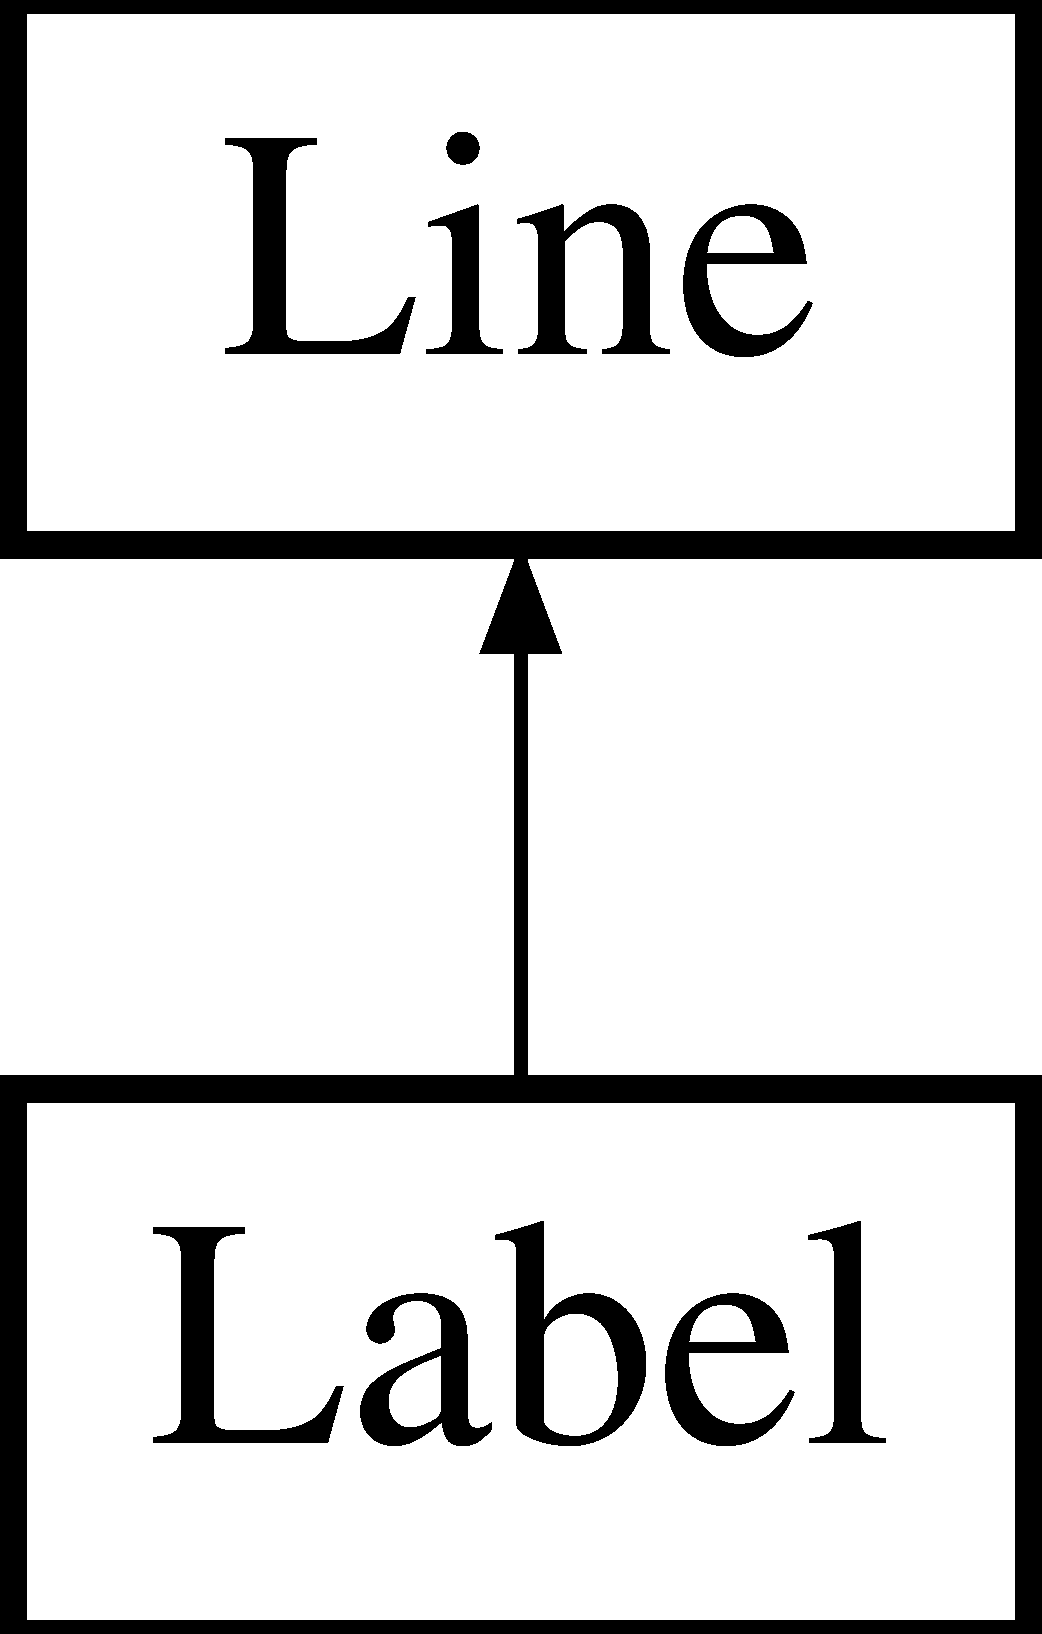
\includegraphics[height=2.000000cm]{class_label}
\end{center}
\end{figure}
\subsection*{Public Member Functions}
\begin{DoxyCompactItemize}
\item 
\hypertarget{class_label_a48e774efc0e6e5cd0bf63a94527add17}{}\hyperlink{class_label_a48e774efc0e6e5cd0bf63a94527add17}{Label} (string)\label{class_label_a48e774efc0e6e5cd0bf63a94527add17}

\begin{DoxyCompactList}\small\item\em Constructor of the \hyperlink{class_label}{Label}. \end{DoxyCompactList}\item 
\hypertarget{class_label_ae0405d591a2ff63c03b104435e2a3066}{}virtual \hyperlink{class_label_ae0405d591a2ff63c03b104435e2a3066}{$\sim$\+Label} ()\label{class_label_ae0405d591a2ff63c03b104435e2a3066}

\begin{DoxyCompactList}\small\item\em Destructor of the \hyperlink{class_label}{Label}. \end{DoxyCompactList}\item 
\hypertarget{class_label_afc727d8ae97b32660faf703b30edc77e}{}virtual t\+\_\+\+Line \hyperlink{class_label_afc727d8ae97b32660faf703b30edc77e}{type\+\_\+line} ()\label{class_label_afc727d8ae97b32660faf703b30edc77e}

\begin{DoxyCompactList}\small\item\em get the type of the line \end{DoxyCompactList}\item 
\hypertarget{class_label_a6df2e96366cc459a6a8fa9642a6e69b6}{}virtual string \hyperlink{class_label_a6df2e96366cc459a6a8fa9642a6e69b6}{to\+\_\+string} ()\label{class_label_a6df2e96366cc459a6a8fa9642a6e69b6}

\begin{DoxyCompactList}\small\item\em get the string of \hyperlink{class_label}{Label} \end{DoxyCompactList}\item 
\hypertarget{class_label_a8d48d53b6eb2c6024b7da507bfa5d00b}{}virtual string \hyperlink{class_label_a8d48d53b6eb2c6024b7da507bfa5d00b}{get\+\_\+content} ()\label{class_label_a8d48d53b6eb2c6024b7da507bfa5d00b}

\begin{DoxyCompactList}\small\item\em get the string of the \hyperlink{class_label}{Label} \end{DoxyCompactList}\item 
\hypertarget{class_label_a16f1db5a51a093f3963a2d902bce845f}{}virtual void \hyperlink{class_label_a16f1db5a51a093f3963a2d902bce845f}{set\+\_\+content} (string)\label{class_label_a16f1db5a51a093f3963a2d902bce845f}

\begin{DoxyCompactList}\small\item\em set the string of the \hyperlink{class_label}{Label} \end{DoxyCompactList}\item 
\hypertarget{class_label_af123355b73ac457171c3118052d145ac}{}virtual t\+\_\+\+Inst \hyperlink{class_label_af123355b73ac457171c3118052d145ac}{get\+\_\+type} ()\label{class_label_af123355b73ac457171c3118052d145ac}

\begin{DoxyCompactList}\small\item\em return the type of the instruction \end{DoxyCompactList}\end{DoxyCompactItemize}
\subsection*{Additional Inherited Members}


\subsection{Detailed Description}
class representing an \hyperlink{class_label}{Label} herited by \hyperlink{class_line}{Line} 

The documentation for this class was generated from the following file\+:\begin{DoxyCompactItemize}
\item 
\hyperlink{_label_8h}{Label.\+h}\end{DoxyCompactItemize}

\hypertarget{class_line}{}\section{Line Class Reference}
\label{class_line}\index{Line@{Line}}


Abstract class representing an \hyperlink{class_line}{Line}.  




{\ttfamily \#include $<$Line.\+h$>$}

Inheritance diagram for Line\+:\begin{figure}[H]
\begin{center}
\leavevmode
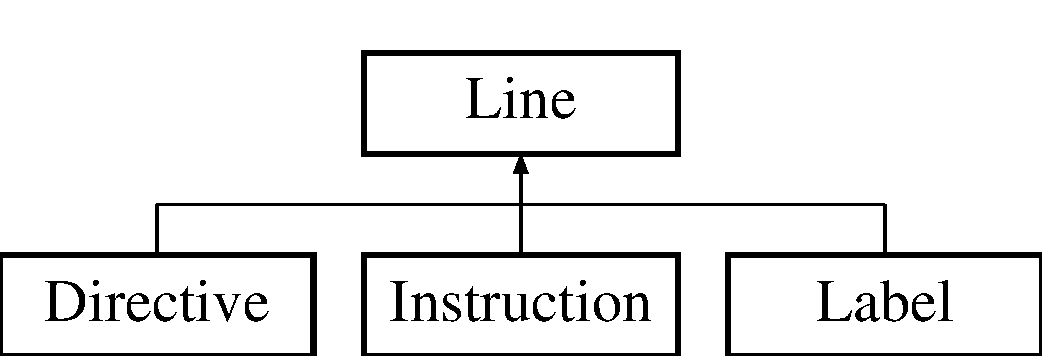
\includegraphics[height=2.000000cm]{class_line}
\end{center}
\end{figure}
\subsection*{Public Member Functions}
\begin{DoxyCompactItemize}
\item 
\hypertarget{class_line_a4a95bafcefa28672b3999deb011b9e50}{}virtual \hyperlink{class_line_a4a95bafcefa28672b3999deb011b9e50}{$\sim$\+Line} ()\label{class_line_a4a95bafcefa28672b3999deb011b9e50}

\begin{DoxyCompactList}\small\item\em Virtual destructor. \end{DoxyCompactList}\item 
\hypertarget{class_line_aa7f74673c9c3a7423a513a5fb64bf825}{}virtual string \hyperlink{class_line_aa7f74673c9c3a7423a513a5fb64bf825}{get\+\_\+content} ()=0\label{class_line_aa7f74673c9c3a7423a513a5fb64bf825}

\begin{DoxyCompactList}\small\item\em get the string of the line virtual getter \end{DoxyCompactList}\item 
\hypertarget{class_line_afa27867ffd08e6915d9e791d2ed0b448}{}virtual void \hyperlink{class_line_afa27867ffd08e6915d9e791d2ed0b448}{set\+\_\+content} (string)=0\label{class_line_afa27867ffd08e6915d9e791d2ed0b448}

\begin{DoxyCompactList}\small\item\em set the string of the line virtual setter \end{DoxyCompactList}\item 
\hypertarget{class_line_a0cc2cdd9bc04649adebd1ff9b753bc85}{}virtual t\+\_\+\+Line \hyperlink{class_line_a0cc2cdd9bc04649adebd1ff9b753bc85}{type\+\_\+line} ()=0\label{class_line_a0cc2cdd9bc04649adebd1ff9b753bc85}

\begin{DoxyCompactList}\small\item\em get the type of the line virtual accessor of the type \end{DoxyCompactList}\item 
virtual string \hyperlink{class_line_a477523118f17d72f58f2912b391afc73}{to\+\_\+string} ()=0
\begin{DoxyCompactList}\small\item\em get the name string accessor of the type line \end{DoxyCompactList}\item 
\hypertarget{class_line_a679ddcc8a7d6a634218f177b4d602bd5}{}virtual t\+\_\+\+Inst \hyperlink{class_line_a679ddcc8a7d6a634218f177b4d602bd5}{get\+\_\+type} ()=0\label{class_line_a679ddcc8a7d6a634218f177b4d602bd5}

\begin{DoxyCompactList}\small\item\em return the type of the instruction \end{DoxyCompactList}\item 
\hypertarget{class_line_a57e724949fa0828dfdd2a1bb0f7db8d0}{}bool \hyperlink{class_line_a57e724949fa0828dfdd2a1bb0f7db8d0}{is\+Inst} ()\label{class_line_a57e724949fa0828dfdd2a1bb0f7db8d0}

\begin{DoxyCompactList}\small\item\em tests if the line is an instruction \end{DoxyCompactList}\item 
\hypertarget{class_line_a8323f3df960924826199bd607198ac7f}{}bool \hyperlink{class_line_a8323f3df960924826199bd607198ac7f}{is\+Label} ()\label{class_line_a8323f3df960924826199bd607198ac7f}

\begin{DoxyCompactList}\small\item\em tests if the line is a label \end{DoxyCompactList}\item 
\hypertarget{class_line_ad014e40a75c8a04e6a091ae4110579bc}{}bool \hyperlink{class_line_ad014e40a75c8a04e6a091ae4110579bc}{is\+Directive} ()\label{class_line_ad014e40a75c8a04e6a091ae4110579bc}

\begin{DoxyCompactList}\small\item\em tests if the line is a directive \end{DoxyCompactList}\item 
\hypertarget{class_line_a66770cb09833f18ec4d5b494f5edae77}{}void \hyperlink{class_line_a66770cb09833f18ec4d5b494f5edae77}{set\+\_\+next} (\hyperlink{class_line}{Line} $\ast$newsuccessor)\label{class_line_a66770cb09833f18ec4d5b494f5edae77}

\begin{DoxyCompactList}\small\item\em set the next line \end{DoxyCompactList}\item 
\hypertarget{class_line_ae834b48e9f1c9450f93ec7bb6a43fb1a}{}\hyperlink{class_line}{Line} $\ast$ \hyperlink{class_line_ae834b48e9f1c9450f93ec7bb6a43fb1a}{get\+\_\+prev} ()\label{class_line_ae834b48e9f1c9450f93ec7bb6a43fb1a}

\begin{DoxyCompactList}\small\item\em get the previous line \end{DoxyCompactList}\item 
\hypertarget{class_line_abf7301d0514bf6dafdc9da9ad79a4341}{}void \hyperlink{class_line_abf7301d0514bf6dafdc9da9ad79a4341}{set\+\_\+prev} (\hyperlink{class_line}{Line} $\ast$newprev)\label{class_line_abf7301d0514bf6dafdc9da9ad79a4341}

\begin{DoxyCompactList}\small\item\em set the previous line \end{DoxyCompactList}\item 
\hypertarget{class_line_a51b6d0f3c36a6aefb03be582277ca570}{}\hyperlink{class_line}{Line} $\ast$ \hyperlink{class_line_a51b6d0f3c36a6aefb03be582277ca570}{get\+\_\+next} ()\label{class_line_a51b6d0f3c36a6aefb03be582277ca570}

\begin{DoxyCompactList}\small\item\em get the next line \end{DoxyCompactList}\end{DoxyCompactItemize}
\subsection*{Protected Attributes}
\begin{DoxyCompactItemize}
\item 
\hypertarget{class_line_aa37e3e0b9ec8180ba796fcd970186437}{}\hyperlink{class_line}{Line} $\ast$ {\bfseries \+\_\+next}\label{class_line_aa37e3e0b9ec8180ba796fcd970186437}

\item 
\hypertarget{class_line_a13163a448797ff8bc4f113202a6d4d4a}{}\hyperlink{class_line}{Line} $\ast$ {\bfseries \+\_\+prev}\label{class_line_a13163a448797ff8bc4f113202a6d4d4a}

\item 
\hypertarget{class_line_a41059923f5c8e5a0f4f44d84bd8762aa}{}string {\bfseries \+\_\+line}\label{class_line_a41059923f5c8e5a0f4f44d84bd8762aa}

\end{DoxyCompactItemize}


\subsection{Detailed Description}
Abstract class representing an \hyperlink{class_line}{Line}. 

\subsection{Member Function Documentation}
\hypertarget{class_line_a477523118f17d72f58f2912b391afc73}{}\index{Line@{Line}!to\+\_\+string@{to\+\_\+string}}
\index{to\+\_\+string@{to\+\_\+string}!Line@{Line}}
\subsubsection[{to\+\_\+string()=0}]{\setlength{\rightskip}{0pt plus 5cm}virtual string Line\+::to\+\_\+string (
\begin{DoxyParamCaption}
{}
\end{DoxyParamCaption}
)\hspace{0.3cm}{\ttfamily [pure virtual]}}\label{class_line_a477523118f17d72f58f2912b391afc73}


get the name string accessor of the type line 



Implemented in \hyperlink{class_instruction_aed87de5e9259f4f15dc885425528f1fe}{Instruction}, \hyperlink{class_directive_a2fd56d5580ad7a993782649d7867732f}{Directive}, and \hyperlink{class_label_a6df2e96366cc459a6a8fa9642a6e69b6}{Label}.



The documentation for this class was generated from the following file\+:\begin{DoxyCompactItemize}
\item 
\hyperlink{_line_8h}{Line.\+h}\end{DoxyCompactItemize}

\hypertarget{class_node__dfg}{}\section{Node\+\_\+dfg Class Reference}
\label{class_node__dfg}\index{Node\+\_\+dfg@{Node\+\_\+dfg}}


class representing a node of data flow graph  




{\ttfamily \#include $<$Node\+\_\+dfg.\+h$>$}

\subsection*{Public Member Functions}
\begin{DoxyCompactItemize}
\item 
\hypertarget{class_node__dfg_ac9b79961aaadf29eecd03b227b4c0875}{}\hyperlink{class_node__dfg_ac9b79961aaadf29eecd03b227b4c0875}{Node\+\_\+dfg} (\hyperlink{class_instruction}{Instruction} $\ast$)\label{class_node__dfg_ac9b79961aaadf29eecd03b227b4c0875}

\begin{DoxyCompactList}\small\item\em Constructor of \hyperlink{class_node__dfg}{Node\+\_\+dfg}. \end{DoxyCompactList}\item 
\hypertarget{class_node__dfg_a0a2a7c4634ad6802e7c69ab0d95957fa}{}\hyperlink{class_node__dfg_a0a2a7c4634ad6802e7c69ab0d95957fa}{$\sim$\+Node\+\_\+dfg} ()\label{class_node__dfg_a0a2a7c4634ad6802e7c69ab0d95957fa}

\begin{DoxyCompactList}\small\item\em Destructor of \hyperlink{class_node__dfg}{Node\+\_\+dfg}. \end{DoxyCompactList}\item 
\hypertarget{class_node__dfg_adc4a8e37604e57eec03fecaaca094fb5}{}\hyperlink{struct_arc__t}{Arc\+\_\+t} $\ast$ \hyperlink{class_node__dfg_adc4a8e37604e57eec03fecaaca094fb5}{get\+\_\+arc} (int i)\label{class_node__dfg_adc4a8e37604e57eec03fecaaca094fb5}

\begin{DoxyCompactList}\small\item\em get the ith arc of the arc list \end{DoxyCompactList}\item 
\hypertarget{class_node__dfg_a27b393ab78abb865ef7c4e494de894da}{}void {\bfseries remove\+\_\+arc} (int index)\label{class_node__dfg_a27b393ab78abb865ef7c4e494de894da}

\item 
\hypertarget{class_node__dfg_a0f65316cde0b35e7755d4ebf009b009b}{}void {\bfseries remove\+\_\+pred} (int index)\label{class_node__dfg_a0f65316cde0b35e7755d4ebf009b009b}

\item 
\hypertarget{class_node__dfg_a6ebd568efb70f729f6e355cdd46a5185}{}list$<$ \hyperlink{struct_arc__t}{Arc\+\_\+t} $\ast$ $>$\+::iterator {\bfseries arcs\+\_\+begin} ()\label{class_node__dfg_a6ebd568efb70f729f6e355cdd46a5185}

\item 
\hypertarget{class_node__dfg_a5a49217bcb16aaf7e94e4e156d9a9d53}{}list$<$ \hyperlink{struct_arc__t}{Arc\+\_\+t} $\ast$ $>$\+::iterator {\bfseries arcs\+\_\+end} ()\label{class_node__dfg_a5a49217bcb16aaf7e94e4e156d9a9d53}

\item 
\hypertarget{class_node__dfg_a85d42a5cc1d6feacf403a8569a813074}{}int \hyperlink{class_node__dfg_a85d42a5cc1d6feacf403a8569a813074}{get\+\_\+nb\+\_\+arcs} ()\label{class_node__dfg_a85d42a5cc1d6feacf403a8569a813074}

\begin{DoxyCompactList}\small\item\em get the number of arcs \end{DoxyCompactList}\item 
\hypertarget{class_node__dfg_a8f20c21a0ffb2e224cc426148362c249}{}\hyperlink{class_instruction}{Instruction} $\ast$ \hyperlink{class_node__dfg_a8f20c21a0ffb2e224cc426148362c249}{get\+\_\+instruction} ()\label{class_node__dfg_a8f20c21a0ffb2e224cc426148362c249}

\begin{DoxyCompactList}\small\item\em get the \hyperlink{class_instruction}{Instruction} \end{DoxyCompactList}\item 
\hypertarget{class_node__dfg_add9d669804bc8ad4a4b806221d9ef9e9}{}void \hyperlink{class_node__dfg_add9d669804bc8ad4a4b806221d9ef9e9}{add\+\_\+successeur} (\hyperlink{struct_arc__t}{Arc\+\_\+t} $\ast$)\label{class_node__dfg_add9d669804bc8ad4a4b806221d9ef9e9}

\begin{DoxyCompactList}\small\item\em add an arc to the arc list \end{DoxyCompactList}\item 
\hypertarget{class_node__dfg_a8cc89b32dbe15bcf399725955a643551}{}void \hyperlink{class_node__dfg_a8cc89b32dbe15bcf399725955a643551}{add\+\_\+predecesseur} (\hyperlink{class_node__dfg}{Node\+\_\+dfg} $\ast$)\label{class_node__dfg_a8cc89b32dbe15bcf399725955a643551}

\begin{DoxyCompactList}\small\item\em add a predecessor to the predecessor list \end{DoxyCompactList}\item 
\hypertarget{class_node__dfg_adef5e6e3362133f6adb38d404c8d8cf6}{}int \hyperlink{class_node__dfg_adef5e6e3362133f6adb38d404c8d8cf6}{nb\+\_\+preds} ()\label{class_node__dfg_adef5e6e3362133f6adb38d404c8d8cf6}

\begin{DoxyCompactList}\small\item\em get the number of predecessors \end{DoxyCompactList}\item 
\hypertarget{class_node__dfg_a769af0d7836679d6ee9abcc55d399887}{}list$<$ \hyperlink{class_node__dfg}{Node\+\_\+dfg} $\ast$ $>$\+::iterator {\bfseries pred\+\_\+begin} ()\label{class_node__dfg_a769af0d7836679d6ee9abcc55d399887}

\item 
\hypertarget{class_node__dfg_a86fc141e0697ae944900625212579957}{}list$<$ \hyperlink{class_node__dfg}{Node\+\_\+dfg} $\ast$ $>$\+::iterator {\bfseries pred\+\_\+end} ()\label{class_node__dfg_a86fc141e0697ae944900625212579957}

\item 
\hypertarget{class_node__dfg_a83747917d9c87b11633779731bcda162}{}void \hyperlink{class_node__dfg_a83747917d9c87b11633779731bcda162}{set\+\_\+instruction} (\hyperlink{class_instruction}{Instruction} $\ast$)\label{class_node__dfg_a83747917d9c87b11633779731bcda162}

\begin{DoxyCompactList}\small\item\em set the \hyperlink{class_instruction}{Instruction} \end{DoxyCompactList}\item 
\hypertarget{class_node__dfg_a395b778a0b23ae2bcfd6081d84661239}{}int {\bfseries compute\+\_\+weight} ()\label{class_node__dfg_a395b778a0b23ae2bcfd6081d84661239}

\item 
\hypertarget{class_node__dfg_af23f48b1521a90178cc5c9a59da3ab3c}{}void \hyperlink{class_node__dfg_af23f48b1521a90178cc5c9a59da3ab3c}{set\+\_\+weight} (int)\label{class_node__dfg_af23f48b1521a90178cc5c9a59da3ab3c}

\begin{DoxyCompactList}\small\item\em set the weight \end{DoxyCompactList}\item 
\hypertarget{class_node__dfg_a561e80f51cb9a71b22f22e8d2e6685de}{}int \hyperlink{class_node__dfg_a561e80f51cb9a71b22f22e8d2e6685de}{get\+\_\+weight} ()\label{class_node__dfg_a561e80f51cb9a71b22f22e8d2e6685de}

\begin{DoxyCompactList}\small\item\em get the weight \end{DoxyCompactList}\item 
\hypertarget{class_node__dfg_a613aa3ee9ce2eb99df07258cbdd5293f}{}int {\bfseries compute\+\_\+nb\+\_\+descendant} (int nb\+\_\+instr, int $\ast$deja\+\_\+comptes)\label{class_node__dfg_a613aa3ee9ce2eb99df07258cbdd5293f}

\item 
\hypertarget{class_node__dfg_a9aa775f727e6c542cd714894219046f3}{}void \hyperlink{class_node__dfg_a9aa775f727e6c542cd714894219046f3}{set\+\_\+nb\+\_\+descendant} (int)\label{class_node__dfg_a9aa775f727e6c542cd714894219046f3}

\begin{DoxyCompactList}\small\item\em set the number of descendant \end{DoxyCompactList}\item 
\hypertarget{class_node__dfg_a9baa0a6be056b7d1ee290c404f2216f5}{}int \hyperlink{class_node__dfg_a9baa0a6be056b7d1ee290c404f2216f5}{get\+\_\+nb\+\_\+descendant} ()\label{class_node__dfg_a9baa0a6be056b7d1ee290c404f2216f5}

\begin{DoxyCompactList}\small\item\em get the number of descendant \end{DoxyCompactList}\item 
\hypertarget{class_node__dfg_ad9fe88cf90fa2282806edbc64f51331e}{}void {\bfseries set\+\_\+tready} (int t)\label{class_node__dfg_ad9fe88cf90fa2282806edbc64f51331e}

\item 
\hypertarget{class_node__dfg_a05e8db316dd2db8b0946167763585c7b}{}int {\bfseries get\+\_\+tready} ()\label{class_node__dfg_a05e8db316dd2db8b0946167763585c7b}

\end{DoxyCompactItemize}


\subsection{Detailed Description}
class representing a node of data flow graph 

The documentation for this class was generated from the following file\+:\begin{DoxyCompactItemize}
\item 
\hyperlink{_node__dfg_8h}{Node\+\_\+dfg.\+h}\end{DoxyCompactItemize}

\hypertarget{class_operand}{}\section{Operand Class Reference}
\label{class_operand}\index{Operand@{Operand}}


Abstract class representing an operand.  




{\ttfamily \#include $<$Operand.\+h$>$}

Inheritance diagram for Operand\+:\begin{figure}[H]
\begin{center}
\leavevmode
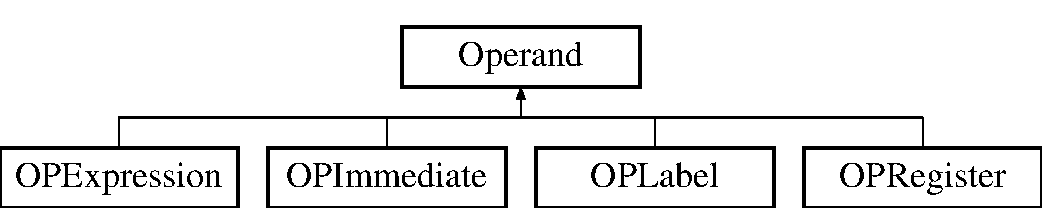
\includegraphics[height=2.000000cm]{class_operand}
\end{center}
\end{figure}
\subsection*{Public Member Functions}
\begin{DoxyCompactItemize}
\item 
\hypertarget{class_operand_aa6ef1ffa183381edb413f9b93782a67b}{}virtual \hyperlink{class_operand_aa6ef1ffa183381edb413f9b93782a67b}{$\sim$\+Operand} ()\label{class_operand_aa6ef1ffa183381edb413f9b93782a67b}

\begin{DoxyCompactList}\small\item\em Virtual destructor. \end{DoxyCompactList}\item 
\hypertarget{class_operand_a2bf3ad8b34d39cb35ff743ffcc0f4675}{}virtual string \hyperlink{class_operand_a2bf3ad8b34d39cb35ff743ffcc0f4675}{get\+\_\+op} ()=0\label{class_operand_a2bf3ad8b34d39cb35ff743ffcc0f4675}

\begin{DoxyCompactList}\small\item\em Get the operand value virtual accessor of the operand. \end{DoxyCompactList}\item 
\hypertarget{class_operand_a0895c39d7b97ea56f074d242e8232c78}{}virtual void \hyperlink{class_operand_a0895c39d7b97ea56f074d242e8232c78}{set\+\_\+op} (string)=0\label{class_operand_a0895c39d7b97ea56f074d242e8232c78}

\begin{DoxyCompactList}\small\item\em set the operand value virtual setter of the operand \end{DoxyCompactList}\item 
virtual t\+\_\+\+Op\+Type \hyperlink{class_operand_afd469e305a467e2574f34ac9bd6c62b0}{get\+\_\+op\+\_\+type} ()=0
\begin{DoxyCompactList}\small\item\em get the operator type virtual accessor of accessor \end{DoxyCompactList}\item 
virtual string \hyperlink{class_operand_a28aed96d5fafee66be81c30c1435ad00}{to\+\_\+string} ()=0
\begin{DoxyCompactList}\small\item\em virtual tostring \end{DoxyCompactList}\item 
\hypertarget{class_operand_a12ccf172b496bc2fee04f732d144641b}{}bool {\bfseries is\+O\+P\+Label} ()\label{class_operand_a12ccf172b496bc2fee04f732d144641b}

\item 
\hypertarget{class_operand_a5c596cb4bdb24227118697d33d9833eb}{}bool {\bfseries is\+O\+P\+Register} ()\label{class_operand_a5c596cb4bdb24227118697d33d9833eb}

\item 
\hypertarget{class_operand_a91f072d08b59eaa343e512e644c8efb4}{}bool {\bfseries is\+O\+P\+Immediate} ()\label{class_operand_a91f072d08b59eaa343e512e644c8efb4}

\end{DoxyCompactItemize}
\subsection*{Protected Attributes}
\begin{DoxyCompactItemize}
\item 
\hypertarget{class_operand_af70a183445064a0106d41dfeea681790}{}string {\bfseries \+\_\+oper}\label{class_operand_af70a183445064a0106d41dfeea681790}

\end{DoxyCompactItemize}


\subsection{Detailed Description}
Abstract class representing an operand. 

\subsection{Member Function Documentation}
\hypertarget{class_operand_afd469e305a467e2574f34ac9bd6c62b0}{}\index{Operand@{Operand}!get\+\_\+op\+\_\+type@{get\+\_\+op\+\_\+type}}
\index{get\+\_\+op\+\_\+type@{get\+\_\+op\+\_\+type}!Operand@{Operand}}
\subsubsection[{get\+\_\+op\+\_\+type()=0}]{\setlength{\rightskip}{0pt plus 5cm}virtual t\+\_\+\+Op\+Type Operand\+::get\+\_\+op\+\_\+type (
\begin{DoxyParamCaption}
{}
\end{DoxyParamCaption}
)\hspace{0.3cm}{\ttfamily [pure virtual]}}\label{class_operand_afd469e305a467e2574f34ac9bd6c62b0}


get the operator type virtual accessor of accessor 

\begin{DoxyReturn}{Returns}
return the \hyperlink{class_operand}{Operand} type as enum 
\end{DoxyReturn}


Implemented in \hyperlink{class_o_p_register_a1be03d6e6422510a1fd12d1f13dfd601}{O\+P\+Register}, \hyperlink{class_o_p_immediate_aed01353798ae57936a9f77dd05eafa88}{O\+P\+Immediate}, \hyperlink{class_o_p_expression_a06f8902130516437d5d93c43a5efcbd2}{O\+P\+Expression}, and \hyperlink{class_o_p_label_a1a6ec701c549a6475d44ffcced1c23b5}{O\+P\+Label}.

\hypertarget{class_operand_a28aed96d5fafee66be81c30c1435ad00}{}\index{Operand@{Operand}!to\+\_\+string@{to\+\_\+string}}
\index{to\+\_\+string@{to\+\_\+string}!Operand@{Operand}}
\subsubsection[{to\+\_\+string()=0}]{\setlength{\rightskip}{0pt plus 5cm}virtual string Operand\+::to\+\_\+string (
\begin{DoxyParamCaption}
{}
\end{DoxyParamCaption}
)\hspace{0.3cm}{\ttfamily [pure virtual]}}\label{class_operand_a28aed96d5fafee66be81c30c1435ad00}


virtual tostring 

\begin{DoxyReturn}{Returns}
return the Object as string 
\end{DoxyReturn}


Implemented in \hyperlink{class_o_p_register_a9f55bdff75224fb18973a9e913a4022f}{O\+P\+Register}, \hyperlink{class_o_p_immediate_a12bc613de3bff73ead8632dafd8050a0}{O\+P\+Immediate}, \hyperlink{class_o_p_expression_a0a6ee03eb083791028eeae021f4ff47b}{O\+P\+Expression}, and \hyperlink{class_o_p_label_a51c4e8f45422f03edcb71d472cf5e973}{O\+P\+Label}.



The documentation for this class was generated from the following file\+:\begin{DoxyCompactItemize}
\item 
\hyperlink{_operand_8h}{Operand.\+h}\end{DoxyCompactItemize}

\hypertarget{class_o_p_expression}{}\section{O\+P\+Expression Class Reference}
\label{class_o_p_expression}\index{O\+P\+Expression@{O\+P\+Expression}}


class representing an expression herited by \hyperlink{class_operand}{Operand}  




{\ttfamily \#include $<$O\+P\+Expression.\+h$>$}

Inheritance diagram for O\+P\+Expression\+:\begin{figure}[H]
\begin{center}
\leavevmode
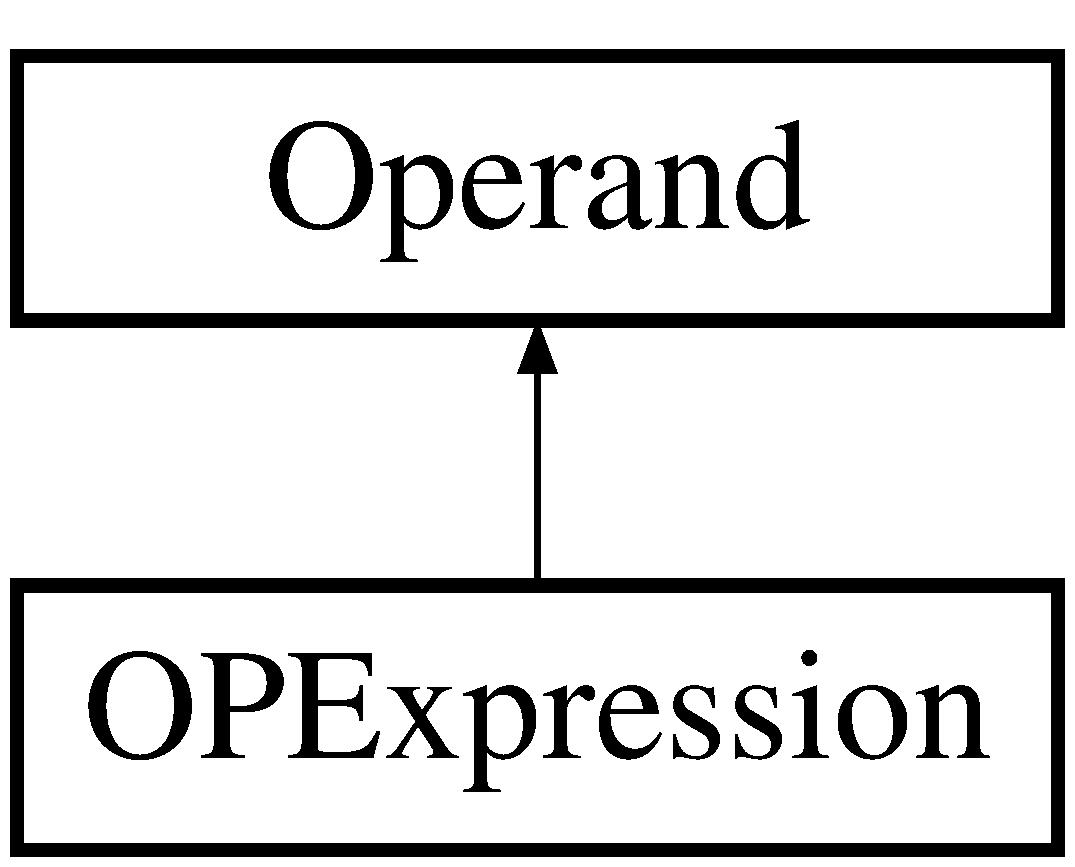
\includegraphics[height=2.000000cm]{class_o_p_expression}
\end{center}
\end{figure}
\subsection*{Public Member Functions}
\begin{DoxyCompactItemize}
\item 
\hypertarget{class_o_p_expression_a5784034daef8568869fe0bb5ecfbcdcf}{}\hyperlink{class_o_p_expression_a5784034daef8568869fe0bb5ecfbcdcf}{O\+P\+Expression} (string)\label{class_o_p_expression_a5784034daef8568869fe0bb5ecfbcdcf}

\begin{DoxyCompactList}\small\item\em Constructor of the Expression class. \end{DoxyCompactList}\item 
\hypertarget{class_o_p_expression_a5ea892d89208ccb593510ee63ef42a19}{}virtual \hyperlink{class_o_p_expression_a5ea892d89208ccb593510ee63ef42a19}{$\sim$\+O\+P\+Expression} ()\label{class_o_p_expression_a5ea892d89208ccb593510ee63ef42a19}

\begin{DoxyCompactList}\small\item\em Destructor of the Expression class. \end{DoxyCompactList}\item 
virtual string \hyperlink{class_o_p_expression_acf86deca614626b803bc3c29facbefef}{get\+\_\+op} ()
\begin{DoxyCompactList}\small\item\em Get the operand value. \end{DoxyCompactList}\item 
virtual t\+\_\+\+Op\+Type \hyperlink{class_o_p_expression_a06f8902130516437d5d93c43a5efcbd2}{get\+\_\+op\+\_\+type} ()
\begin{DoxyCompactList}\small\item\em get the operator type \end{DoxyCompactList}\item 
virtual string \hyperlink{class_o_p_expression_a0a6ee03eb083791028eeae021f4ff47b}{to\+\_\+string} ()
\begin{DoxyCompactList}\small\item\em tostring \end{DoxyCompactList}\item 
\hypertarget{class_o_p_expression_a3cfeacf4f76611d374be3caa9de80a05}{}virtual void \hyperlink{class_o_p_expression_a3cfeacf4f76611d374be3caa9de80a05}{set\+\_\+op} (string)\label{class_o_p_expression_a3cfeacf4f76611d374be3caa9de80a05}

\begin{DoxyCompactList}\small\item\em set the operand value setter of the operand \end{DoxyCompactList}\end{DoxyCompactItemize}
\subsection*{Additional Inherited Members}


\subsection{Detailed Description}
class representing an expression herited by \hyperlink{class_operand}{Operand} 

\subsection{Member Function Documentation}
\hypertarget{class_o_p_expression_acf86deca614626b803bc3c29facbefef}{}\index{O\+P\+Expression@{O\+P\+Expression}!get\+\_\+op@{get\+\_\+op}}
\index{get\+\_\+op@{get\+\_\+op}!O\+P\+Expression@{O\+P\+Expression}}
\subsubsection[{get\+\_\+op()}]{\setlength{\rightskip}{0pt plus 5cm}virtual string O\+P\+Expression\+::get\+\_\+op (
\begin{DoxyParamCaption}
{}
\end{DoxyParamCaption}
)\hspace{0.3cm}{\ttfamily [virtual]}}\label{class_o_p_expression_acf86deca614626b803bc3c29facbefef}


Get the operand value. 

\begin{DoxyReturn}{Returns}
return the string of the Expression 
\end{DoxyReturn}


Implements \hyperlink{class_operand_a2bf3ad8b34d39cb35ff743ffcc0f4675}{Operand}.

\hypertarget{class_o_p_expression_a06f8902130516437d5d93c43a5efcbd2}{}\index{O\+P\+Expression@{O\+P\+Expression}!get\+\_\+op\+\_\+type@{get\+\_\+op\+\_\+type}}
\index{get\+\_\+op\+\_\+type@{get\+\_\+op\+\_\+type}!O\+P\+Expression@{O\+P\+Expression}}
\subsubsection[{get\+\_\+op\+\_\+type()}]{\setlength{\rightskip}{0pt plus 5cm}virtual t\+\_\+\+Op\+Type O\+P\+Expression\+::get\+\_\+op\+\_\+type (
\begin{DoxyParamCaption}
{}
\end{DoxyParamCaption}
)\hspace{0.3cm}{\ttfamily [virtual]}}\label{class_o_p_expression_a06f8902130516437d5d93c43a5efcbd2}


get the operator type 

\begin{DoxyReturn}{Returns}
return the \hyperlink{class_operand}{Operand} type as enum 
\end{DoxyReturn}


Implements \hyperlink{class_operand_afd469e305a467e2574f34ac9bd6c62b0}{Operand}.

\hypertarget{class_o_p_expression_a0a6ee03eb083791028eeae021f4ff47b}{}\index{O\+P\+Expression@{O\+P\+Expression}!to\+\_\+string@{to\+\_\+string}}
\index{to\+\_\+string@{to\+\_\+string}!O\+P\+Expression@{O\+P\+Expression}}
\subsubsection[{to\+\_\+string()}]{\setlength{\rightskip}{0pt plus 5cm}virtual string O\+P\+Expression\+::to\+\_\+string (
\begin{DoxyParamCaption}
{}
\end{DoxyParamCaption}
)\hspace{0.3cm}{\ttfamily [virtual]}}\label{class_o_p_expression_a0a6ee03eb083791028eeae021f4ff47b}


tostring 

\begin{DoxyReturn}{Returns}
return the Object as string 
\end{DoxyReturn}


Implements \hyperlink{class_operand_a28aed96d5fafee66be81c30c1435ad00}{Operand}.



The documentation for this class was generated from the following file\+:\begin{DoxyCompactItemize}
\item 
\hyperlink{_o_p_expression_8h}{O\+P\+Expression.\+h}\end{DoxyCompactItemize}

\hypertarget{class_o_p_immediate}{}\section{O\+P\+Immediate Class Reference}
\label{class_o_p_immediate}\index{O\+P\+Immediate@{O\+P\+Immediate}}


class representing an Immediate herited by \hyperlink{class_operand}{Operand}  




{\ttfamily \#include $<$O\+P\+Immediate.\+h$>$}

Inheritance diagram for O\+P\+Immediate\+:\begin{figure}[H]
\begin{center}
\leavevmode
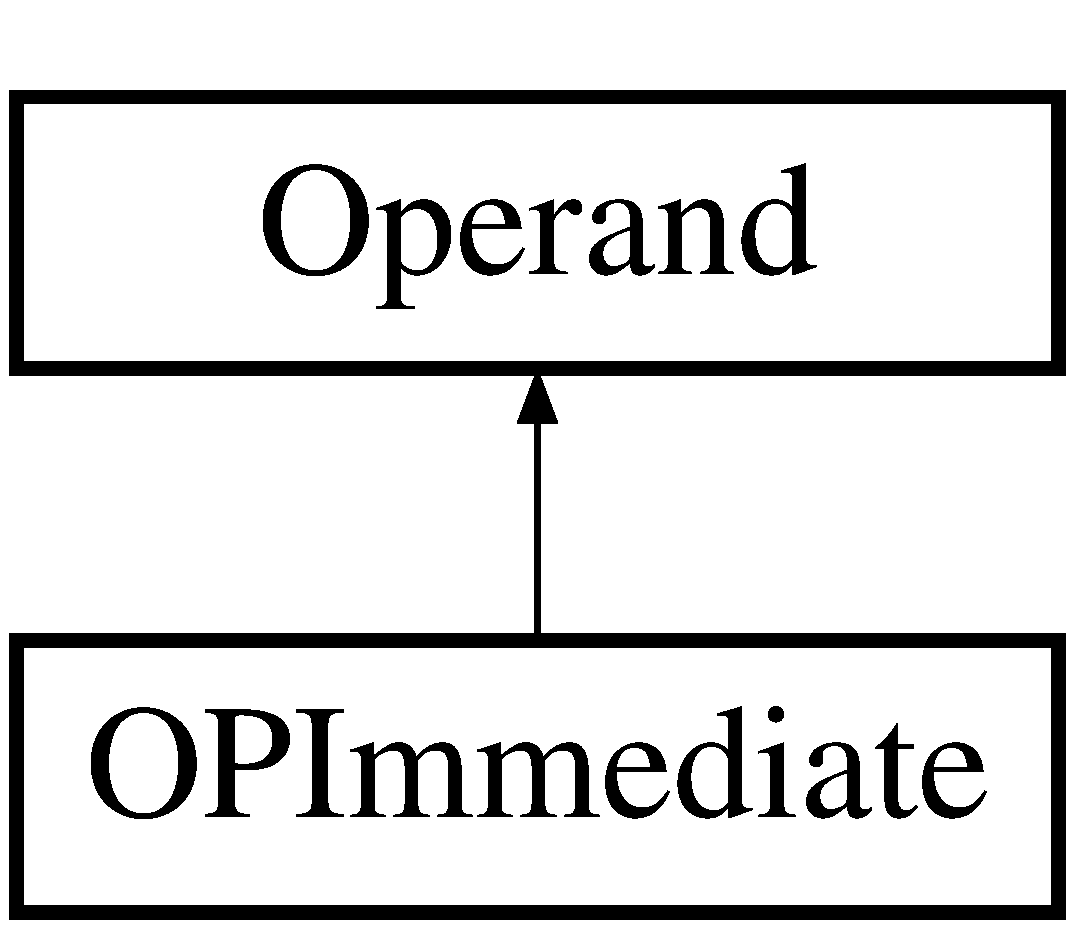
\includegraphics[height=2.000000cm]{class_o_p_immediate}
\end{center}
\end{figure}
\subsection*{Public Member Functions}
\begin{DoxyCompactItemize}
\item 
\hypertarget{class_o_p_immediate_ab047dac5f3390947a21e4ab118c05857}{}\hyperlink{class_o_p_immediate_ab047dac5f3390947a21e4ab118c05857}{O\+P\+Immediate} (string)\label{class_o_p_immediate_ab047dac5f3390947a21e4ab118c05857}

\begin{DoxyCompactList}\small\item\em Constructor of the Immediate Class. \end{DoxyCompactList}\item 
\hypertarget{class_o_p_immediate_ae940dcf9e9050227a94c759a0cae6861}{}\hyperlink{class_o_p_immediate_ae940dcf9e9050227a94c759a0cae6861}{O\+P\+Immediate} (int)\label{class_o_p_immediate_ae940dcf9e9050227a94c759a0cae6861}

\begin{DoxyCompactList}\small\item\em Constructor of the Immediate Class. \end{DoxyCompactList}\item 
\hypertarget{class_o_p_immediate_af7f51ae61e075e02817d6ecd7441408f}{}virtual \hyperlink{class_o_p_immediate_af7f51ae61e075e02817d6ecd7441408f}{$\sim$\+O\+P\+Immediate} ()\label{class_o_p_immediate_af7f51ae61e075e02817d6ecd7441408f}

\begin{DoxyCompactList}\small\item\em Destructor of the Immediate Class. \end{DoxyCompactList}\item 
virtual string \hyperlink{class_o_p_immediate_ad714fb614c0d8f4afa1157a34b2936fd}{get\+\_\+op} ()
\begin{DoxyCompactList}\small\item\em Get the string of the operand. \end{DoxyCompactList}\item 
virtual t\+\_\+\+Op\+Type \hyperlink{class_o_p_immediate_aed01353798ae57936a9f77dd05eafa88}{get\+\_\+op\+\_\+type} ()
\begin{DoxyCompactList}\small\item\em get the operator type \end{DoxyCompactList}\item 
virtual string \hyperlink{class_o_p_immediate_a12bc613de3bff73ead8632dafd8050a0}{to\+\_\+string} ()
\begin{DoxyCompactList}\small\item\em tostring \end{DoxyCompactList}\item 
\hypertarget{class_o_p_immediate_ae5d6c30c6bff17de4e7fabb24cf6bf59}{}virtual void \hyperlink{class_o_p_immediate_ae5d6c30c6bff17de4e7fabb24cf6bf59}{set\+\_\+op} (string)\label{class_o_p_immediate_ae5d6c30c6bff17de4e7fabb24cf6bf59}

\begin{DoxyCompactList}\small\item\em set the string of the operand setter of the operand \end{DoxyCompactList}\end{DoxyCompactItemize}
\subsection*{Additional Inherited Members}


\subsection{Detailed Description}
class representing an Immediate herited by \hyperlink{class_operand}{Operand} 

\subsection{Member Function Documentation}
\hypertarget{class_o_p_immediate_ad714fb614c0d8f4afa1157a34b2936fd}{}\index{O\+P\+Immediate@{O\+P\+Immediate}!get\+\_\+op@{get\+\_\+op}}
\index{get\+\_\+op@{get\+\_\+op}!O\+P\+Immediate@{O\+P\+Immediate}}
\subsubsection[{get\+\_\+op()}]{\setlength{\rightskip}{0pt plus 5cm}virtual string O\+P\+Immediate\+::get\+\_\+op (
\begin{DoxyParamCaption}
{}
\end{DoxyParamCaption}
)\hspace{0.3cm}{\ttfamily [virtual]}}\label{class_o_p_immediate_ad714fb614c0d8f4afa1157a34b2936fd}


Get the string of the operand. 

\begin{DoxyReturn}{Returns}
return the string of the Immediate 
\end{DoxyReturn}


Implements \hyperlink{class_operand_a2bf3ad8b34d39cb35ff743ffcc0f4675}{Operand}.

\hypertarget{class_o_p_immediate_aed01353798ae57936a9f77dd05eafa88}{}\index{O\+P\+Immediate@{O\+P\+Immediate}!get\+\_\+op\+\_\+type@{get\+\_\+op\+\_\+type}}
\index{get\+\_\+op\+\_\+type@{get\+\_\+op\+\_\+type}!O\+P\+Immediate@{O\+P\+Immediate}}
\subsubsection[{get\+\_\+op\+\_\+type()}]{\setlength{\rightskip}{0pt plus 5cm}virtual t\+\_\+\+Op\+Type O\+P\+Immediate\+::get\+\_\+op\+\_\+type (
\begin{DoxyParamCaption}
{}
\end{DoxyParamCaption}
)\hspace{0.3cm}{\ttfamily [virtual]}}\label{class_o_p_immediate_aed01353798ae57936a9f77dd05eafa88}


get the operator type 

\begin{DoxyReturn}{Returns}
return the \hyperlink{class_operand}{Operand} type as enum 
\end{DoxyReturn}


Implements \hyperlink{class_operand_afd469e305a467e2574f34ac9bd6c62b0}{Operand}.

\hypertarget{class_o_p_immediate_a12bc613de3bff73ead8632dafd8050a0}{}\index{O\+P\+Immediate@{O\+P\+Immediate}!to\+\_\+string@{to\+\_\+string}}
\index{to\+\_\+string@{to\+\_\+string}!O\+P\+Immediate@{O\+P\+Immediate}}
\subsubsection[{to\+\_\+string()}]{\setlength{\rightskip}{0pt plus 5cm}virtual string O\+P\+Immediate\+::to\+\_\+string (
\begin{DoxyParamCaption}
{}
\end{DoxyParamCaption}
)\hspace{0.3cm}{\ttfamily [virtual]}}\label{class_o_p_immediate_a12bc613de3bff73ead8632dafd8050a0}


tostring 

\begin{DoxyReturn}{Returns}
return the name of the Object as string 
\end{DoxyReturn}


Implements \hyperlink{class_operand_a28aed96d5fafee66be81c30c1435ad00}{Operand}.



The documentation for this class was generated from the following file\+:\begin{DoxyCompactItemize}
\item 
\hyperlink{_o_p_immediate_8h}{O\+P\+Immediate.\+h}\end{DoxyCompactItemize}

\hypertarget{class_o_p_label}{}\section{O\+P\+Label Class Reference}
\label{class_o_p_label}\index{O\+P\+Label@{O\+P\+Label}}


class representing a \hyperlink{class_label}{Label} herited by \hyperlink{class_operand}{Operand}  




{\ttfamily \#include $<$O\+P\+Label.\+h$>$}

Inheritance diagram for O\+P\+Label\+:\begin{figure}[H]
\begin{center}
\leavevmode
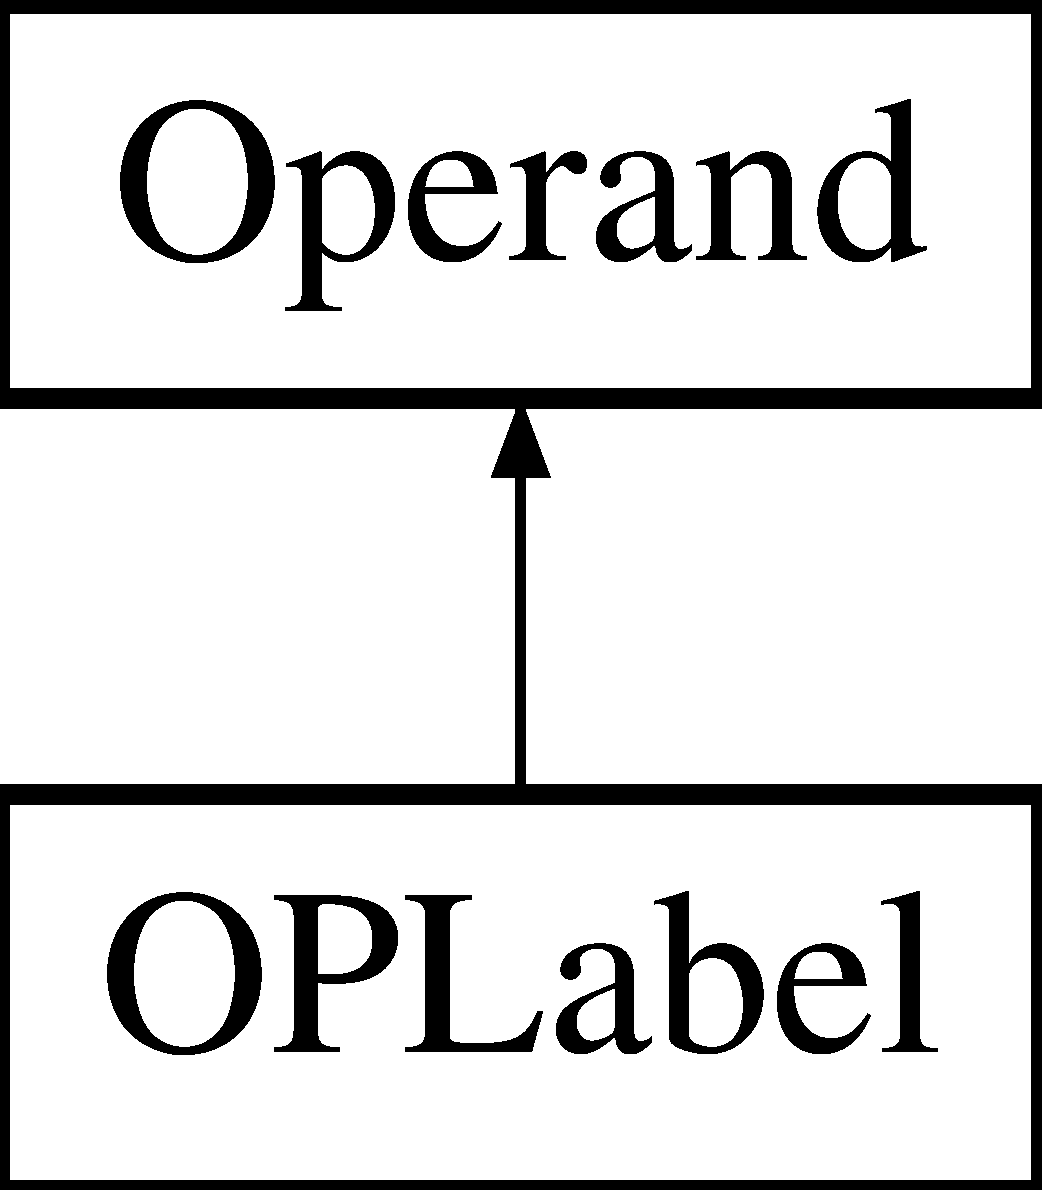
\includegraphics[height=2.000000cm]{class_o_p_label}
\end{center}
\end{figure}
\subsection*{Public Member Functions}
\begin{DoxyCompactItemize}
\item 
\hypertarget{class_o_p_label_a5405b78894658047362a328e750f88b4}{}\hyperlink{class_o_p_label_a5405b78894658047362a328e750f88b4}{O\+P\+Label} (string)\label{class_o_p_label_a5405b78894658047362a328e750f88b4}

\begin{DoxyCompactList}\small\item\em Constructor of the \hyperlink{class_label}{Label} Class. \end{DoxyCompactList}\item 
\hypertarget{class_o_p_label_ab25553d41606e880a622e09d5c09129d}{}virtual \hyperlink{class_o_p_label_ab25553d41606e880a622e09d5c09129d}{$\sim$\+O\+P\+Label} ()\label{class_o_p_label_ab25553d41606e880a622e09d5c09129d}

\begin{DoxyCompactList}\small\item\em Destructor of the \hyperlink{class_label}{Label} Class. \end{DoxyCompactList}\item 
\hypertarget{class_o_p_label_a1c933d10a7b2267bae3bea6c385d466f}{}virtual string \hyperlink{class_o_p_label_a1c933d10a7b2267bae3bea6c385d466f}{get\+\_\+op} ()\label{class_o_p_label_a1c933d10a7b2267bae3bea6c385d466f}

\begin{DoxyCompactList}\small\item\em Get the string of the operand accessor of the operand. \end{DoxyCompactList}\item 
virtual t\+\_\+\+Op\+Type \hyperlink{class_o_p_label_a1a6ec701c549a6475d44ffcced1c23b5}{get\+\_\+op\+\_\+type} ()
\begin{DoxyCompactList}\small\item\em get the operator type \end{DoxyCompactList}\item 
virtual string \hyperlink{class_o_p_label_a51c4e8f45422f03edcb71d472cf5e973}{to\+\_\+string} ()
\begin{DoxyCompactList}\small\item\em tostring \end{DoxyCompactList}\item 
\hypertarget{class_o_p_label_a189bec8bcf7300e6e8656ce4bb443995}{}virtual void \hyperlink{class_o_p_label_a189bec8bcf7300e6e8656ce4bb443995}{set\+\_\+op} (string)\label{class_o_p_label_a189bec8bcf7300e6e8656ce4bb443995}

\begin{DoxyCompactList}\small\item\em set the operand value setter of the operand \end{DoxyCompactList}\end{DoxyCompactItemize}
\subsection*{Additional Inherited Members}


\subsection{Detailed Description}
class representing a \hyperlink{class_label}{Label} herited by \hyperlink{class_operand}{Operand} 

\subsection{Member Function Documentation}
\hypertarget{class_o_p_label_a1a6ec701c549a6475d44ffcced1c23b5}{}\index{O\+P\+Label@{O\+P\+Label}!get\+\_\+op\+\_\+type@{get\+\_\+op\+\_\+type}}
\index{get\+\_\+op\+\_\+type@{get\+\_\+op\+\_\+type}!O\+P\+Label@{O\+P\+Label}}
\subsubsection[{get\+\_\+op\+\_\+type()}]{\setlength{\rightskip}{0pt plus 5cm}virtual t\+\_\+\+Op\+Type O\+P\+Label\+::get\+\_\+op\+\_\+type (
\begin{DoxyParamCaption}
{}
\end{DoxyParamCaption}
)\hspace{0.3cm}{\ttfamily [virtual]}}\label{class_o_p_label_a1a6ec701c549a6475d44ffcced1c23b5}


get the operator type 

\begin{DoxyReturn}{Returns}
return the \hyperlink{class_operand}{Operand} type as enum 
\end{DoxyReturn}


Implements \hyperlink{class_operand_afd469e305a467e2574f34ac9bd6c62b0}{Operand}.

\hypertarget{class_o_p_label_a51c4e8f45422f03edcb71d472cf5e973}{}\index{O\+P\+Label@{O\+P\+Label}!to\+\_\+string@{to\+\_\+string}}
\index{to\+\_\+string@{to\+\_\+string}!O\+P\+Label@{O\+P\+Label}}
\subsubsection[{to\+\_\+string()}]{\setlength{\rightskip}{0pt plus 5cm}virtual string O\+P\+Label\+::to\+\_\+string (
\begin{DoxyParamCaption}
{}
\end{DoxyParamCaption}
)\hspace{0.3cm}{\ttfamily [virtual]}}\label{class_o_p_label_a51c4e8f45422f03edcb71d472cf5e973}


tostring 

\begin{DoxyReturn}{Returns}
return the name of the Object as string 
\end{DoxyReturn}


Implements \hyperlink{class_operand_a28aed96d5fafee66be81c30c1435ad00}{Operand}.



The documentation for this class was generated from the following file\+:\begin{DoxyCompactItemize}
\item 
\hyperlink{_o_p_label_8h}{O\+P\+Label.\+h}\end{DoxyCompactItemize}

\hypertarget{class_o_p_register}{}\section{O\+P\+Register Class Reference}
\label{class_o_p_register}\index{O\+P\+Register@{O\+P\+Register}}


class representing a Register herited by \hyperlink{class_operand}{Operand}  




{\ttfamily \#include $<$O\+P\+Register.\+h$>$}

Inheritance diagram for O\+P\+Register\+:\begin{figure}[H]
\begin{center}
\leavevmode
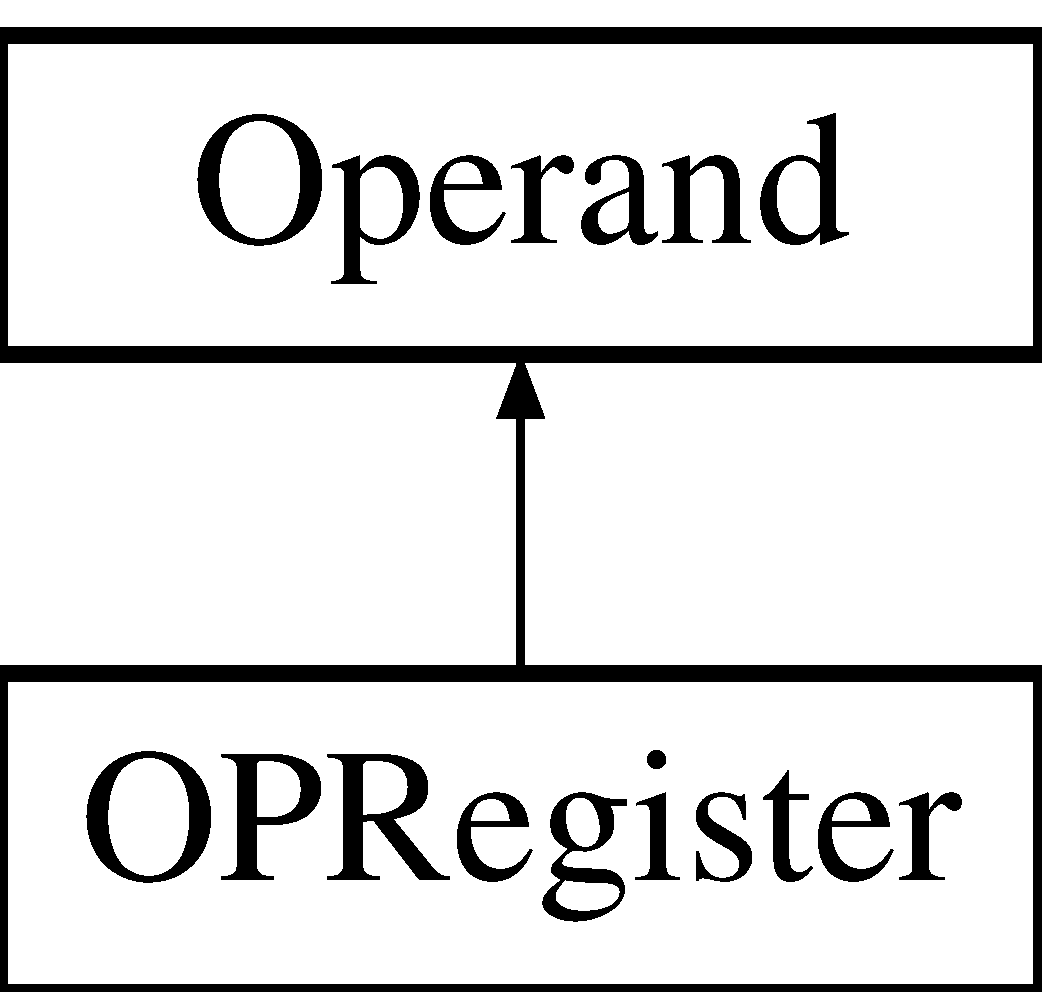
\includegraphics[height=2.000000cm]{class_o_p_register}
\end{center}
\end{figure}
\subsection*{Public Member Functions}
\begin{DoxyCompactItemize}
\item 
\hypertarget{class_o_p_register_a896eb65f36bf615ccfa74541de23858f}{}\hyperlink{class_o_p_register_a896eb65f36bf615ccfa74541de23858f}{O\+P\+Register} (string, t\+\_\+\+Src\+\_\+\+Dst)\label{class_o_p_register_a896eb65f36bf615ccfa74541de23858f}

\begin{DoxyCompactList}\small\item\em Constructor of the Register class. \end{DoxyCompactList}\item 
\hypertarget{class_o_p_register_ad75c23d1db7c149c20cbc8bb01c6df59}{}\hyperlink{class_o_p_register_ad75c23d1db7c149c20cbc8bb01c6df59}{O\+P\+Register} (string, int, t\+\_\+\+Src\+\_\+\+Dst)\label{class_o_p_register_ad75c23d1db7c149c20cbc8bb01c6df59}

\begin{DoxyCompactList}\small\item\em Constructor of the Register class. \end{DoxyCompactList}\item 
\hypertarget{class_o_p_register_a3c9786680764ada47370d469790b8178}{}{\bfseries O\+P\+Register} (int, t\+\_\+\+Src\+\_\+\+Dst)\label{class_o_p_register_a3c9786680764ada47370d469790b8178}

\item 
\hypertarget{class_o_p_register_aedab3bc5a2eecd0d02771fb6b37d73fe}{}virtual \hyperlink{class_o_p_register_aedab3bc5a2eecd0d02771fb6b37d73fe}{$\sim$\+O\+P\+Register} ()\label{class_o_p_register_aedab3bc5a2eecd0d02771fb6b37d73fe}

\begin{DoxyCompactList}\small\item\em Destructor of the Register class. \end{DoxyCompactList}\item 
int \hyperlink{class_o_p_register_a2e42d6407677a7be154a5d4d74f7a8e7}{get\+\_\+reg} ()
\begin{DoxyCompactList}\small\item\em Get the Register value. \end{DoxyCompactList}\item 
\hypertarget{class_o_p_register_ab514f45a9957e9b485fee38f264a70cf}{}void \hyperlink{class_o_p_register_ab514f45a9957e9b485fee38f264a70cf}{set\+\_\+reg} (int)\label{class_o_p_register_ab514f45a9957e9b485fee38f264a70cf}

\begin{DoxyCompactList}\small\item\em set the Register value setter of the Register \end{DoxyCompactList}\item 
virtual string \hyperlink{class_o_p_register_a3f9f6cad40b83eee3f88a2e84a0ccffa}{get\+\_\+op} ()
\begin{DoxyCompactList}\small\item\em Get the operand value. \end{DoxyCompactList}\item 
virtual t\+\_\+\+Op\+Type \hyperlink{class_o_p_register_a1be03d6e6422510a1fd12d1f13dfd601}{get\+\_\+op\+\_\+type} ()
\begin{DoxyCompactList}\small\item\em get the operator type \end{DoxyCompactList}\item 
virtual string \hyperlink{class_o_p_register_a9f55bdff75224fb18973a9e913a4022f}{to\+\_\+string} ()
\begin{DoxyCompactList}\small\item\em tostring \end{DoxyCompactList}\item 
\hypertarget{class_o_p_register_a3cceb6c804e4fe1187de7eb47c21a285}{}virtual void \hyperlink{class_o_p_register_a3cceb6c804e4fe1187de7eb47c21a285}{set\+\_\+op} (string)\label{class_o_p_register_a3cceb6c804e4fe1187de7eb47c21a285}

\begin{DoxyCompactList}\small\item\em set the operand value setter of the operand \end{DoxyCompactList}\item 
\hypertarget{class_o_p_register_a23b5061c12e99d3bd320038e643eb247}{}void \hyperlink{class_o_p_register_a23b5061c12e99d3bd320038e643eb247}{set\+\_\+type} (t\+\_\+\+Src\+\_\+\+Dst)\label{class_o_p_register_a23b5061c12e99d3bd320038e643eb247}

\begin{DoxyCompactList}\small\item\em set the type of the register setter of the register type \end{DoxyCompactList}\item 
\hypertarget{class_o_p_register_a7748867306b20ca99c0955b376789777}{}t\+\_\+\+Src\+\_\+\+Dst \hyperlink{class_o_p_register_a7748867306b20ca99c0955b376789777}{get\+\_\+type} ()\label{class_o_p_register_a7748867306b20ca99c0955b376789777}

\begin{DoxyCompactList}\small\item\em get the type of the register getter of the register type \end{DoxyCompactList}\end{DoxyCompactItemize}
\subsection*{Additional Inherited Members}


\subsection{Detailed Description}
class representing a Register herited by \hyperlink{class_operand}{Operand} 

\subsection{Member Function Documentation}
\hypertarget{class_o_p_register_a3f9f6cad40b83eee3f88a2e84a0ccffa}{}\index{O\+P\+Register@{O\+P\+Register}!get\+\_\+op@{get\+\_\+op}}
\index{get\+\_\+op@{get\+\_\+op}!O\+P\+Register@{O\+P\+Register}}
\subsubsection[{get\+\_\+op()}]{\setlength{\rightskip}{0pt plus 5cm}virtual string O\+P\+Register\+::get\+\_\+op (
\begin{DoxyParamCaption}
{}
\end{DoxyParamCaption}
)\hspace{0.3cm}{\ttfamily [virtual]}}\label{class_o_p_register_a3f9f6cad40b83eee3f88a2e84a0ccffa}


Get the operand value. 

\begin{DoxyReturn}{Returns}
return the string of the register 
\end{DoxyReturn}


Implements \hyperlink{class_operand_a2bf3ad8b34d39cb35ff743ffcc0f4675}{Operand}.

\hypertarget{class_o_p_register_a1be03d6e6422510a1fd12d1f13dfd601}{}\index{O\+P\+Register@{O\+P\+Register}!get\+\_\+op\+\_\+type@{get\+\_\+op\+\_\+type}}
\index{get\+\_\+op\+\_\+type@{get\+\_\+op\+\_\+type}!O\+P\+Register@{O\+P\+Register}}
\subsubsection[{get\+\_\+op\+\_\+type()}]{\setlength{\rightskip}{0pt plus 5cm}virtual t\+\_\+\+Op\+Type O\+P\+Register\+::get\+\_\+op\+\_\+type (
\begin{DoxyParamCaption}
{}
\end{DoxyParamCaption}
)\hspace{0.3cm}{\ttfamily [virtual]}}\label{class_o_p_register_a1be03d6e6422510a1fd12d1f13dfd601}


get the operator type 

\begin{DoxyReturn}{Returns}
return the \hyperlink{class_operand}{Operand} type as enum 
\end{DoxyReturn}


Implements \hyperlink{class_operand_afd469e305a467e2574f34ac9bd6c62b0}{Operand}.

\hypertarget{class_o_p_register_a2e42d6407677a7be154a5d4d74f7a8e7}{}\index{O\+P\+Register@{O\+P\+Register}!get\+\_\+reg@{get\+\_\+reg}}
\index{get\+\_\+reg@{get\+\_\+reg}!O\+P\+Register@{O\+P\+Register}}
\subsubsection[{get\+\_\+reg()}]{\setlength{\rightskip}{0pt plus 5cm}int O\+P\+Register\+::get\+\_\+reg (
\begin{DoxyParamCaption}
{}
\end{DoxyParamCaption}
)}\label{class_o_p_register_a2e42d6407677a7be154a5d4d74f7a8e7}


Get the Register value. 

\begin{DoxyReturn}{Returns}
return the number of the Register 
\end{DoxyReturn}
\hypertarget{class_o_p_register_a9f55bdff75224fb18973a9e913a4022f}{}\index{O\+P\+Register@{O\+P\+Register}!to\+\_\+string@{to\+\_\+string}}
\index{to\+\_\+string@{to\+\_\+string}!O\+P\+Register@{O\+P\+Register}}
\subsubsection[{to\+\_\+string()}]{\setlength{\rightskip}{0pt plus 5cm}virtual string O\+P\+Register\+::to\+\_\+string (
\begin{DoxyParamCaption}
{}
\end{DoxyParamCaption}
)\hspace{0.3cm}{\ttfamily [virtual]}}\label{class_o_p_register_a9f55bdff75224fb18973a9e913a4022f}


tostring 

\begin{DoxyReturn}{Returns}
return the Object as string 
\end{DoxyReturn}


Implements \hyperlink{class_operand_a28aed96d5fafee66be81c30c1435ad00}{Operand}.



The documentation for this class was generated from the following file\+:\begin{DoxyCompactItemize}
\item 
\hyperlink{_o_p_register_8h}{O\+P\+Register.\+h}\end{DoxyCompactItemize}

\hypertarget{class_program}{}\section{Program Class Reference}
\label{class_program}\index{Program@{Program}}


class representing a program as list  




{\ttfamily \#include $<$Program.\+h$>$}

\subsection*{Public Member Functions}
\begin{DoxyCompactItemize}
\item 
\hypertarget{class_program_aaefaa0df08f3484476fc4d61e97acbdc}{}\hyperlink{class_program_aaefaa0df08f3484476fc4d61e97acbdc}{Program} ()\label{class_program_aaefaa0df08f3484476fc4d61e97acbdc}

\begin{DoxyCompactList}\small\item\em Empty constructor of a program. \end{DoxyCompactList}\item 
\hypertarget{class_program_a9918fe797bf830c47a652c81f449c35c}{}\hyperlink{class_program_a9918fe797bf830c47a652c81f449c35c}{Program} (\hyperlink{class_program}{Program} const \&otherprogram)\label{class_program_a9918fe797bf830c47a652c81f449c35c}

\begin{DoxyCompactList}\small\item\em Copy constructor of a program. \end{DoxyCompactList}\item 
\hypertarget{class_program_aabe3dfc72075de14b189b22b0e33ff23}{}\hyperlink{class_program_aabe3dfc72075de14b189b22b0e33ff23}{Program} (string const file)\label{class_program_aabe3dfc72075de14b189b22b0e33ff23}

\begin{DoxyCompactList}\small\item\em Constructor with the input file of program. \end{DoxyCompactList}\item 
\hypertarget{class_program_a986aef1c50e1d338a3315a47ba6df549}{}\hyperlink{class_program_a986aef1c50e1d338a3315a47ba6df549}{$\sim$\+Program} ()\label{class_program_a986aef1c50e1d338a3315a47ba6df549}

\begin{DoxyCompactList}\small\item\em Destructor of program. \end{DoxyCompactList}\item 
\hypertarget{class_program_a90e1c506dffd5756133f70811f6117d9}{}void \hyperlink{class_program_a90e1c506dffd5756133f70811f6117d9}{add\+\_\+line} (\hyperlink{class_line}{Line} $\ast$newline)\label{class_program_a90e1c506dffd5756133f70811f6117d9}

\begin{DoxyCompactList}\small\item\em Add a line at the end of the program. \end{DoxyCompactList}\item 
\hypertarget{class_program_a7adb0709f1a9f3ed63e861cc7f02d308}{}int \hyperlink{class_program_a7adb0709f1a9f3ed63e861cc7f02d308}{add\+\_\+line\+\_\+at} (\hyperlink{class_line}{Line} $\ast$newline, int position)\label{class_program_a7adb0709f1a9f3ed63e861cc7f02d308}

\begin{DoxyCompactList}\small\item\em Add a line to the program with position as index. \end{DoxyCompactList}\item 
\hypertarget{class_program_aabea8add836e10a384b63e2f293ece23}{}void \hyperlink{class_program_aabea8add836e10a384b63e2f293ece23}{exchange\+\_\+line} (int line1, int line2)\label{class_program_aabea8add836e10a384b63e2f293ece23}

\begin{DoxyCompactList}\small\item\em Reverse two lines which are at the index line1 and line2. \end{DoxyCompactList}\item 
\hypertarget{class_program_a3c1399ac5ed69e5c152f1a2cc1e644d4}{}void \hyperlink{class_program_a3c1399ac5ed69e5c152f1a2cc1e644d4}{display} ()\label{class_program_a3c1399ac5ed69e5c152f1a2cc1e644d4}

\begin{DoxyCompactList}\small\item\em display the program \end{DoxyCompactList}\item 
\hypertarget{class_program_a1adce5c1fc414a378e4b87f1d4b535e1}{}void \hyperlink{class_program_a1adce5c1fc414a378e4b87f1d4b535e1}{del\+\_\+line} (int index)\label{class_program_a1adce5c1fc414a378e4b87f1d4b535e1}

\begin{DoxyCompactList}\small\item\em Delete the line at the given index in the program. \end{DoxyCompactList}\item 
\hypertarget{class_program_ae897b48e1e1be99578440eb6a38a3a0d}{}\hyperlink{class_line}{Line} $\ast$ \hyperlink{class_program_ae897b48e1e1be99578440eb6a38a3a0d}{find\+\_\+line} (int index)\label{class_program_ae897b48e1e1be99578440eb6a38a3a0d}

\begin{DoxyCompactList}\small\item\em gives the line that corresponds to the index \end{DoxyCompactList}\item 
\hypertarget{class_program_a190f24ecadca14d748408c352aabc219}{}int \hyperlink{class_program_a190f24ecadca14d748408c352aabc219}{size} ()\label{class_program_a190f24ecadca14d748408c352aabc219}

\begin{DoxyCompactList}\small\item\em get the length of the program \end{DoxyCompactList}\item 
void \hyperlink{class_program_a3db3e17c96bb809c3e6f81b8bc22ee20}{in\+\_\+file} (string const filename)
\begin{DoxyCompactList}\small\item\em returns the dependance betwen the two given instructions \end{DoxyCompactList}\item 
\hypertarget{class_program_aff32c461ae544453df5d55f475b3da22}{}bool \hyperlink{class_program_aff32c461ae544453df5d55f475b3da22}{is\+\_\+empty} ()\label{class_program_aff32c461ae544453df5d55f475b3da22}

\begin{DoxyCompactList}\small\item\em return true if the program is Empty \end{DoxyCompactList}\item 
\hypertarget{class_program_aa2111257b1f690520316e4831e55798d}{}void \hyperlink{class_program_aa2111257b1f690520316e4831e55798d}{comput\+\_\+function} ()\label{class_program_aa2111257b1f690520316e4831e55798d}

\begin{DoxyCompactList}\small\item\em calculate the functions of the program \end{DoxyCompactList}\item 
\hypertarget{class_program_aa85073d3bd6782af3759f4a2961ae80f}{}int \hyperlink{class_program_aa85073d3bd6782af3759f4a2961ae80f}{nbr\+\_\+func} ()\label{class_program_aa85073d3bd6782af3759f4a2961ae80f}

\begin{DoxyCompactList}\small\item\em get the number of functions in the program \end{DoxyCompactList}\item 
\hypertarget{class_program_aea6d5c7367bbee48ec5cbb295ef6fd5f}{}\hyperlink{class_function}{Function} $\ast$ \hyperlink{class_program_aea6d5c7367bbee48ec5cbb295ef6fd5f}{get\+\_\+function} (int index)\label{class_program_aea6d5c7367bbee48ec5cbb295ef6fd5f}

\begin{DoxyCompactList}\small\item\em returns the function of index index in the list \+\_\+myfunc \end{DoxyCompactList}\item 
\hypertarget{class_program_a88b4499bd1a7485d7492fc812b957899}{}list$<$ \hyperlink{class_function}{Function} $\ast$ $>$\+::iterator {\bfseries function\+\_\+list\+\_\+begin} ()\label{class_program_a88b4499bd1a7485d7492fc812b957899}

\item 
\hypertarget{class_program_a7507c914934f6847c6a4e19dae13cdf3}{}list$<$ \hyperlink{class_function}{Function} $\ast$ $>$\+::iterator {\bfseries function\+\_\+list\+\_\+end} ()\label{class_program_a7507c914934f6847c6a4e19dae13cdf3}

\item 
\hypertarget{class_program_a1cef65227311c68a2e81c89dcbc16914}{}void \hyperlink{class_program_a1cef65227311c68a2e81c89dcbc16914}{flush} ()\label{class_program_a1cef65227311c68a2e81c89dcbc16914}

\begin{DoxyCompactList}\small\item\em empty the program \end{DoxyCompactList}\item 
\hypertarget{class_program_a0d1d9386925418b5fd0a09bf5de16208}{}void \hyperlink{class_program_a0d1d9386925418b5fd0a09bf5de16208}{comput\+\_\+\+C\+F\+G} ()\label{class_program_a0d1d9386925418b5fd0a09bf5de16208}

\begin{DoxyCompactList}\small\item\em calculate the C\+F\+G associated with each function of the program \end{DoxyCompactList}\item 
\hypertarget{class_program_a69ddee195c76bff05733d927e315f319}{}\hyperlink{class_cfg}{Cfg} $\ast$ \hyperlink{class_program_a69ddee195c76bff05733d927e315f319}{get\+\_\+\+C\+F\+G} (int index)\label{class_program_a69ddee195c76bff05733d927e315f319}

\begin{DoxyCompactList}\small\item\em returns the C\+F\+G of index index in the list \+\_\+my\+C\+F\+G \end{DoxyCompactList}\end{DoxyCompactItemize}


\subsection{Detailed Description}
class representing a program as list 

\subsection{Member Function Documentation}
\hypertarget{class_program_a3db3e17c96bb809c3e6f81b8bc22ee20}{}\index{Program@{Program}!in\+\_\+file@{in\+\_\+file}}
\index{in\+\_\+file@{in\+\_\+file}!Program@{Program}}
\subsubsection[{in\+\_\+file(string const filename)}]{\setlength{\rightskip}{0pt plus 5cm}void Program\+::in\+\_\+file (
\begin{DoxyParamCaption}
\item[{string const}]{filename}
\end{DoxyParamCaption}
)}\label{class_program_a3db3e17c96bb809c3e6f81b8bc22ee20}


returns the dependance betwen the two given instructions 

\begin{DoxyReturn}{Returns}
returns the dependance in the enum formatwrite the programme into a file 
\end{DoxyReturn}


The documentation for this class was generated from the following file\+:\begin{DoxyCompactItemize}
\item 
\hyperlink{_program_8h}{Program.\+h}\end{DoxyCompactItemize}

\hypertarget{structs___profile}{}\section{s\+\_\+\+Profile Struct Reference}
\label{structs___profile}\index{s\+\_\+\+Profile@{s\+\_\+\+Profile}}


Structure allowing to add caracteristics to an operator.  




{\ttfamily \#include $<$Enum\+\_\+type.\+h$>$}

\subsection*{Public Attributes}
\begin{DoxyCompactItemize}
\item 
\hypertarget{structs___profile_a3debabafa904b8f4c5e7bf2bda2a5e60}{}t\+\_\+\+Operator {\bfseries op}\label{structs___profile_a3debabafa904b8f4c5e7bf2bda2a5e60}

\item 
\hypertarget{structs___profile_ab9f52013690834dd36766d356c90c449}{}std\+::string {\bfseries nom}\label{structs___profile_ab9f52013690834dd36766d356c90c449}

\item 
\hypertarget{structs___profile_ae8153795530389f76f6c56bdeac40d46}{}t\+\_\+\+Format {\bfseries format}\label{structs___profile_ae8153795530389f76f6c56bdeac40d46}

\item 
\hypertarget{structs___profile_a2a8c53bcb4fb28c3aa368a27954d9b1b}{}t\+\_\+\+Inst {\bfseries type}\label{structs___profile_a2a8c53bcb4fb28c3aa368a27954d9b1b}

\item 
\hypertarget{structs___profile_a7930c41fdfa4249a1c147edf7ac68822}{}int {\bfseries nb\+\_\+oper}\label{structs___profile_a7930c41fdfa4249a1c147edf7ac68822}

\end{DoxyCompactItemize}


\subsection{Detailed Description}
Structure allowing to add caracteristics to an operator. 

The documentation for this struct was generated from the following file\+:\begin{DoxyCompactItemize}
\item 
Enum\+\_\+type.\+h\end{DoxyCompactItemize}

\hypertarget{class_test_o_p_label}{}\section{Test\+O\+P\+Label Class Reference}
\label{class_test_o_p_label}\index{Test\+O\+P\+Label@{Test\+O\+P\+Label}}
Inheritance diagram for Test\+O\+P\+Label\+:\begin{figure}[H]
\begin{center}
\leavevmode
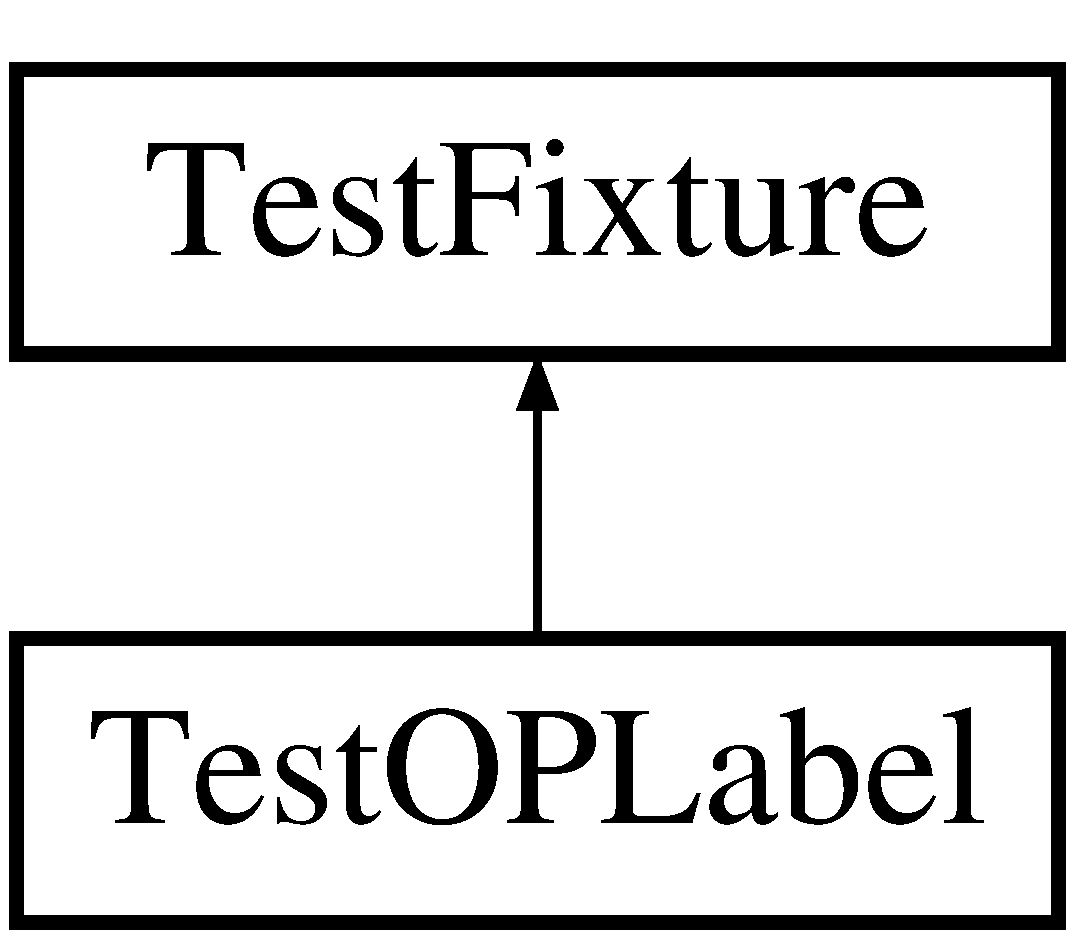
\includegraphics[height=2.000000cm]{class_test_o_p_label}
\end{center}
\end{figure}
\subsection*{Public Member Functions}
\begin{DoxyCompactItemize}
\item 
\hypertarget{class_test_o_p_label_a9ddb0e7ab19700d5bf73490ba0ebbf36}{}void {\bfseries set\+Up} (void)\label{class_test_o_p_label_a9ddb0e7ab19700d5bf73490ba0ebbf36}

\item 
\hypertarget{class_test_o_p_label_a6bc3fb561309973920fe3abc020facf1}{}void {\bfseries tear\+Down} (void)\label{class_test_o_p_label_a6bc3fb561309973920fe3abc020facf1}

\end{DoxyCompactItemize}


The documentation for this class was generated from the following file\+:\begin{DoxyCompactItemize}
\item 
Test\+O\+P\+Label.\+h\end{DoxyCompactItemize}

\hypertarget{structutchn}{}\section{utchn Struct Reference}
\label{structutchn}\index{utchn@{utchn}}
\subsection*{Public Attributes}
\begin{DoxyCompactItemize}
\item 
\hypertarget{structutchn_adf89384022b2de9cb3a0be987e746bbe}{}struct \hyperlink{structutchn}{utchn} $\ast$ {\bfseries N\+E\+X\+T}\label{structutchn_adf89384022b2de9cb3a0be987e746bbe}

\item 
\hypertarget{structutchn_a4c8453ea9877abcfdb65a88f3497a294}{}union \hyperlink{unionutdat}{utdat} {\bfseries D\+A\+T\+A}\label{structutchn_a4c8453ea9877abcfdb65a88f3497a294}

\end{DoxyCompactItemize}


The documentation for this struct was generated from the following file\+:\begin{DoxyCompactItemize}
\item 
utl200.\+h\end{DoxyCompactItemize}

\hypertarget{unionutdat}{}\section{utdat Union Reference}
\label{unionutdat}\index{utdat@{utdat}}
\subsection*{Public Attributes}
\begin{DoxyCompactItemize}
\item 
\hypertarget{unionutdat_a3f76aa32eacd8c9a18af99d01be467c2}{}void $\ast$ {\bfseries V\+P\+N\+T}\label{unionutdat_a3f76aa32eacd8c9a18af99d01be467c2}

\item 
\hypertarget{unionutdat_ae0e7486135096802136dc1cd41c9a005}{}float {\bfseries F\+L\+O\+T}\label{unionutdat_ae0e7486135096802136dc1cd41c9a005}

\item 
\hypertarget{unionutdat_aae5fc4b76253540a8c4e983e162072be}{}unsigned int {\bfseries U\+I\+N\+T}\label{unionutdat_aae5fc4b76253540a8c4e983e162072be}

\item 
\hypertarget{unionutdat_a5bf144421cb7bf3264438be37aa5d884}{}int {\bfseries S\+I\+N\+T}\label{unionutdat_a5bf144421cb7bf3264438be37aa5d884}

\item 
\hypertarget{unionutdat_afad7210b163e44fc45ba5d19f9354b73}{}char {\bfseries C\+H\+A\+R}\label{unionutdat_afad7210b163e44fc45ba5d19f9354b73}

\item 
\hypertarget{unionutdat_ac716e252c27e7f050371d9c28b4c75f4}{}unsigned char {\bfseries U\+C\+H\+R}\label{unionutdat_ac716e252c27e7f050371d9c28b4c75f4}

\end{DoxyCompactItemize}


The documentation for this union was generated from the following file\+:\begin{DoxyCompactItemize}
\item 
utl200.\+h\end{DoxyCompactItemize}

\hypertarget{structutdic}{}\section{utdic Struct Reference}
\label{structutdic}\index{utdic@{utdic}}
\subsection*{Public Attributes}
\begin{DoxyCompactItemize}
\item 
\hypertarget{structutdic_afa286d4adfb2ac8a02c022cc635057b0}{}struct \hyperlink{structutdic}{utdic} $\ast$ {\bfseries N\+E\+X\+T}\label{structutdic_afa286d4adfb2ac8a02c022cc635057b0}

\item 
\hypertarget{structutdic_a04eed0ebafe9ecb10bf6126f332f4969}{}struct \hyperlink{structutdit}{utdit} $\ast$ {\bfseries T\+A\+B\+L\+E}\label{structutdic_a04eed0ebafe9ecb10bf6126f332f4969}

\item 
\hypertarget{structutdic_a5726659f4bf5e8bc5c32a08f4d941719}{}void $\ast$($\ast$ {\bfseries A\+D\+D\+\_\+\+K} )()\label{structutdic_a5726659f4bf5e8bc5c32a08f4d941719}

\item 
\hypertarget{structutdic_ad9ee2cdae45e36b1c6c8de47f81898e7}{}void($\ast$ {\bfseries F\+R\+E\+\_\+\+K} )()\label{structutdic_ad9ee2cdae45e36b1c6c8de47f81898e7}

\item 
\hypertarget{structutdic_a811ec079161985fbdb39e4c064ab5b0d}{}int($\ast$ {\bfseries C\+M\+P\+\_\+\+K} )()\label{structutdic_a811ec079161985fbdb39e4c064ab5b0d}

\item 
\hypertarget{structutdic_a14014c24853e69cd1c5bc6ca7cb776bc}{}void $\ast$($\ast$ {\bfseries A\+D\+D\+\_\+\+D} )()\label{structutdic_a14014c24853e69cd1c5bc6ca7cb776bc}

\item 
\hypertarget{structutdic_a4d4de487f7be4ec26ef0cb193cc32c3d}{}void($\ast$ {\bfseries F\+R\+E\+\_\+\+D} )()\label{structutdic_a4d4de487f7be4ec26ef0cb193cc32c3d}

\item 
\hypertarget{structutdic_ad7407cf1b683d16fb1025967d21c1237}{}unsigned int($\ast$ {\bfseries H\+S\+H\+\_\+\+K} )()\label{structutdic_ad7407cf1b683d16fb1025967d21c1237}

\item 
\hypertarget{structutdic_a55eabe5e987e0fbe7683b3c938390e56}{}unsigned short {\bfseries S\+I\+Z\+E}\label{structutdic_a55eabe5e987e0fbe7683b3c938390e56}

\item 
\hypertarget{structutdic_a797453db20732c62ffb3603de50d88a9}{}unsigned short {\bfseries S\+P\+E\+E\+D}\label{structutdic_a797453db20732c62ffb3603de50d88a9}

\item 
\hypertarget{structutdic_a5ac9d099e722a47666b07c10f155b503}{}unsigned int {\bfseries I\+N\+I\+T}\label{structutdic_a5ac9d099e722a47666b07c10f155b503}

\item 
\hypertarget{structutdic_a66864a2a75e70334df90b8fb4dff592f}{}unsigned int {\bfseries S\+T\+A\+T\+U\+S}\label{structutdic_a66864a2a75e70334df90b8fb4dff592f}

\item 
\hypertarget{structutdic_a1cc5230f2a4edd235bbcb11ba492c5a9}{}unsigned int {\bfseries F\+L\+A\+G}\label{structutdic_a1cc5230f2a4edd235bbcb11ba492c5a9}

\end{DoxyCompactItemize}


The documentation for this struct was generated from the following file\+:\begin{DoxyCompactItemize}
\item 
utl200.\+h\end{DoxyCompactItemize}

\hypertarget{structutdit}{}\section{utdit Struct Reference}
\label{structutdit}\index{utdit@{utdit}}
\subsection*{Public Attributes}
\begin{DoxyCompactItemize}
\item 
\hypertarget{structutdit_a35be07ef8c6bf95874e1569b1c2a446a}{}struct \hyperlink{structuttyp}{uttyp} $\ast$ {\bfseries I\+T\+E\+M}\label{structutdit_a35be07ef8c6bf95874e1569b1c2a446a}

\end{DoxyCompactItemize}


The documentation for this struct was generated from the following file\+:\begin{DoxyCompactItemize}
\item 
utl200.\+h\end{DoxyCompactItemize}

\hypertarget{structuttdc}{}\section{uttdc Struct Reference}
\label{structuttdc}\index{uttdc@{uttdc}}
\subsection*{Public Attributes}
\begin{DoxyCompactItemize}
\item 
\hypertarget{structuttdc_a36ecbdb0a7090fabe5bfdafe71d29e1c}{}struct \hyperlink{structuttdc}{uttdc} $\ast$ {\bfseries N\+E\+X\+T}\label{structuttdc_a36ecbdb0a7090fabe5bfdafe71d29e1c}

\item 
\hypertarget{structuttdc_ad03c46371086203aa425921abb0e39ef}{}union \hyperlink{unionutdat}{utdat} {\bfseries D\+A\+T1}\label{structuttdc_ad03c46371086203aa425921abb0e39ef}

\item 
\hypertarget{structuttdc_adce9c114f323143827917a9ba99db1b4}{}union \hyperlink{unionutdat}{utdat} {\bfseries D\+A\+T2}\label{structuttdc_adce9c114f323143827917a9ba99db1b4}

\item 
\hypertarget{structuttdc_ae45fd296fefee3b446fa004fae80b737}{}union \hyperlink{unionutdat}{utdat} {\bfseries D\+A\+T3}\label{structuttdc_ae45fd296fefee3b446fa004fae80b737}

\end{DoxyCompactItemize}


The documentation for this struct was generated from the following file\+:\begin{DoxyCompactItemize}
\item 
utl200.\+h\end{DoxyCompactItemize}

\hypertarget{structuttpd}{}\section{uttpd Struct Reference}
\label{structuttpd}\index{uttpd@{uttpd}}
\subsection*{Public Attributes}
\begin{DoxyCompactItemize}
\item 
\hypertarget{structuttpd_a5cb5f6e1386d4d1a421db63a9f296879}{}struct \hyperlink{structuttpd}{uttpd} $\ast$ {\bfseries N\+E\+X\+T}\label{structuttpd_a5cb5f6e1386d4d1a421db63a9f296879}

\item 
\hypertarget{structuttpd_a5dc0039ca809f7aa4f582b830c005762}{}union \hyperlink{unionutdat}{utdat} {\bfseries D\+A\+T1}\label{structuttpd_a5dc0039ca809f7aa4f582b830c005762}

\item 
\hypertarget{structuttpd_adaea4e4a8db887e61b8944d75c5be2a3}{}double {\bfseries D\+A\+T2}\label{structuttpd_adaea4e4a8db887e61b8944d75c5be2a3}

\end{DoxyCompactItemize}


The documentation for this struct was generated from the following file\+:\begin{DoxyCompactItemize}
\item 
utl200.\+h\end{DoxyCompactItemize}

\hypertarget{structuttyp}{}\section{uttyp Struct Reference}
\label{structuttyp}\index{uttyp@{uttyp}}
\subsection*{Public Attributes}
\begin{DoxyCompactItemize}
\item 
\hypertarget{structuttyp_aeb2e67b550626f318c8627127cac0f10}{}struct \hyperlink{structuttyp}{uttyp} $\ast$ {\bfseries N\+E\+X\+T}\label{structuttyp_aeb2e67b550626f318c8627127cac0f10}

\item 
\hypertarget{structuttyp_a8c93cab3549706951c3785e1aec42242}{}union \hyperlink{unionutdat}{utdat} {\bfseries D\+A\+T1}\label{structuttyp_a8c93cab3549706951c3785e1aec42242}

\item 
\hypertarget{structuttyp_a8d2dd6929a5e74e498543bf759ba1bea}{}union \hyperlink{unionutdat}{utdat} {\bfseries D\+A\+T2}\label{structuttyp_a8d2dd6929a5e74e498543bf759ba1bea}

\end{DoxyCompactItemize}


The documentation for this struct was generated from the following file\+:\begin{DoxyCompactItemize}
\item 
utl200.\+h\end{DoxyCompactItemize}

\hypertarget{union_y_y_s_t_y_p_e}{}\section{Y\+Y\+S\+T\+Y\+P\+E Union Reference}
\label{union_y_y_s_t_y_p_e}\index{Y\+Y\+S\+T\+Y\+P\+E@{Y\+Y\+S\+T\+Y\+P\+E}}
\subsection*{Public Attributes}
\begin{DoxyCompactItemize}
\item 
\hypertarget{union_y_y_s_t_y_p_e_a4b9cb65f9c58be454aa7c4b25698d709}{}struct \hyperlink{structutchn}{utchn} $\ast$ {\bfseries pchn}\label{union_y_y_s_t_y_p_e_a4b9cb65f9c58be454aa7c4b25698d709}

\item 
\hypertarget{union_y_y_s_t_y_p_e_a8ea73faccde5303458c8eae598a8bef4}{}unsigned int {\bfseries uval}\label{union_y_y_s_t_y_p_e_a8ea73faccde5303458c8eae598a8bef4}

\item 
\hypertarget{union_y_y_s_t_y_p_e_a9208e91d3ca5483b43d8c1fbd7be4ce6}{}char $\ast$ {\bfseries text}\label{union_y_y_s_t_y_p_e_a9208e91d3ca5483b43d8c1fbd7be4ce6}

\end{DoxyCompactItemize}


The documentation for this union was generated from the following file\+:\begin{DoxyCompactItemize}
\item 
asm\+\_\+mipsyac.\+h\end{DoxyCompactItemize}

\chapter{File Documentation}
\hypertarget{_basic__block_8h}{}\section{Basic\+\_\+block.\+h File Reference}
\label{_basic__block_8h}\index{Basic\+\_\+block.\+h@{Basic\+\_\+block.\+h}}


\hyperlink{class_basic__block}{Basic\+\_\+block} class.  


{\ttfamily \#include $<$Line.\+h$>$}\\*
{\ttfamily \#include $<$Instruction.\+h$>$}\\*
{\ttfamily \#include $<$string$>$}\\*
{\ttfamily \#include $<$stdio.\+h$>$}\\*
{\ttfamily \#include $<$Enum\+\_\+type.\+h$>$}\\*
{\ttfamily \#include $<$fstream$>$}\\*
{\ttfamily \#include $<$vector$>$}\\*
{\ttfamily \#include $<$list$>$}\\*
{\ttfamily \#include $<$Dfg.\+h$>$}\\*
{\ttfamily \#include $<$Node\+\_\+dfg.\+h$>$}\\*
\subsection*{Classes}
\begin{DoxyCompactItemize}
\item 
class \hyperlink{class_basic__block}{Basic\+\_\+block}
\begin{DoxyCompactList}\small\item\em class representing a \hyperlink{class_basic__block}{Basic\+\_\+block} of a fonction \end{DoxyCompactList}\end{DoxyCompactItemize}


\subsection{Detailed Description}
\hyperlink{class_basic__block}{Basic\+\_\+block} class. 

\begin{DoxyAuthor}{Author}
Hajjem 
\end{DoxyAuthor}

\hypertarget{_cfg_8h}{}\section{Cfg.\+h File Reference}
\label{_cfg_8h}\index{Cfg.\+h@{Cfg.\+h}}


\hyperlink{class_cfg}{Cfg} class.  


{\ttfamily \#include $<$Basic\+\_\+block.\+h$>$}\\*
{\ttfamily \#include $<$string$>$}\\*
{\ttfamily \#include $<$stdio.\+h$>$}\\*
{\ttfamily \#include $<$Label.\+h$>$}\\*
{\ttfamily \#include $<$Enum\+\_\+type.\+h$>$}\\*
{\ttfamily \#include $<$list$>$}\\*
{\ttfamily \#include $<$fstream$>$}\\*
\subsection*{Classes}
\begin{DoxyCompactItemize}
\item 
class \hyperlink{class_cfg}{Cfg}
\begin{DoxyCompactList}\small\item\em class representing control flow graph \end{DoxyCompactList}\end{DoxyCompactItemize}


\subsection{Detailed Description}
\hyperlink{class_cfg}{Cfg} class. 

\begin{DoxyAuthor}{Author}
Hajjem 
\end{DoxyAuthor}

\hypertarget{_dfg_8h}{}\section{Dfg.\+h File Reference}
\label{_dfg_8h}\index{Dfg.\+h@{Dfg.\+h}}


\hyperlink{class_dfg}{Dfg} class.  


{\ttfamily \#include $<$Node\+\_\+dfg.\+h$>$}\\*
{\ttfamily \#include $<$Instruction.\+h$>$}\\*
{\ttfamily \#include $<$Enum\+\_\+type.\+h$>$}\\*
{\ttfamily \#include $<$fstream$>$}\\*
{\ttfamily \#include $<$list$>$}\\*
{\ttfamily \#include $<$boost/graph/adjacency\+\_\+list.\+hpp$>$}\\*
{\ttfamily \#include $<$boost/graph/astar\+\_\+search.\+hpp$>$}\\*
\subsection*{Classes}
\begin{DoxyCompactItemize}
\item 
class \hyperlink{class_dfg}{Dfg}
\begin{DoxyCompactList}\small\item\em class representing a \hyperlink{class_dfg}{Dfg} of a Basic block, a data flow graph that is to be used to calculate the critical path and schedule code \end{DoxyCompactList}\end{DoxyCompactItemize}


\subsection{Detailed Description}
\hyperlink{class_dfg}{Dfg} class. 


\hypertarget{_directive_8h}{}\section{Directive.\+h File Reference}
\label{_directive_8h}\index{Directive.\+h@{Directive.\+h}}


\hyperlink{class_directive}{Directive} class.  


{\ttfamily \#include $<$iostream$>$}\\*
{\ttfamily \#include $<$string$>$}\\*
{\ttfamily \#include $<$Enum\+\_\+type.\+h$>$}\\*
{\ttfamily \#include $<$Line.\+h$>$}\\*
\subsection*{Classes}
\begin{DoxyCompactItemize}
\item 
class \hyperlink{class_directive}{Directive}
\begin{DoxyCompactList}\small\item\em class representing an \hyperlink{class_directive}{Directive} herited by \hyperlink{class_line}{Line} \end{DoxyCompactList}\end{DoxyCompactItemize}
\subsection*{Functions}
\begin{DoxyCompactItemize}
\item 
\hypertarget{_directive_8h_a0f34d943225eea7b4ffdb6107a79fff1}{}\hyperlink{class_directive}{Directive} $\ast$ \hyperlink{_directive_8h_a0f34d943225eea7b4ffdb6107a79fff1}{get\+Directive} (\hyperlink{class_line}{Line} $\ast$l)\label{_directive_8h_a0f34d943225eea7b4ffdb6107a79fff1}

\begin{DoxyCompactList}\small\item\em returns the \hyperlink{class_directive}{Directive} associated to the line, if the line is a directive, N\+U\+L\+L otherwise \end{DoxyCompactList}\end{DoxyCompactItemize}


\subsection{Detailed Description}
\hyperlink{class_directive}{Directive} class. 

\begin{DoxyAuthor}{Author}
Hajjem 
\end{DoxyAuthor}

\hypertarget{_function_8h}{}\section{Function.\+h File Reference}
\label{_function_8h}\index{Function.\+h@{Function.\+h}}


\hyperlink{class_function}{Function} class.  


{\ttfamily \#include $<$Line.\+h$>$}\\*
{\ttfamily \#include $<$Basic\+\_\+block.\+h$>$}\\*
{\ttfamily \#include $<$Instruction.\+h$>$}\\*
{\ttfamily \#include $<$string$>$}\\*
{\ttfamily \#include $<$stdio.\+h$>$}\\*
{\ttfamily \#include $<$Label.\+h$>$}\\*
{\ttfamily \#include $<$Enum\+\_\+type.\+h$>$}\\*
{\ttfamily \#include $<$list$>$}\\*
{\ttfamily \#include $<$Cfg.\+h$>$}\\*
{\ttfamily \#include $<$fstream$>$}\\*
\subsection*{Classes}
\begin{DoxyCompactItemize}
\item 
class \hyperlink{class_function}{Function}
\begin{DoxyCompactList}\small\item\em class representing a \hyperlink{class_function}{Function} on a program \end{DoxyCompactList}\end{DoxyCompactItemize}


\subsection{Detailed Description}
\hyperlink{class_function}{Function} class. 

\begin{DoxyAuthor}{Author}
Hajjem 
\end{DoxyAuthor}

\hypertarget{_instruction_8h}{}\section{Instruction.\+h File Reference}
\label{_instruction_8h}\index{Instruction.\+h@{Instruction.\+h}}


\hyperlink{class_instruction}{Instruction} class.  


{\ttfamily \#include $<$Operand.\+h$>$}\\*
{\ttfamily \#include $<$string$>$}\\*
{\ttfamily \#include $<$O\+P\+Expression.\+h$>$}\\*
{\ttfamily \#include $<$O\+P\+Immediate.\+h$>$}\\*
{\ttfamily \#include $<$O\+P\+Label.\+h$>$}\\*
{\ttfamily \#include $<$Line.\+h$>$}\\*
{\ttfamily \#include $<$O\+P\+Register.\+h$>$}\\*
{\ttfamily \#include $<$Enum\+\_\+type.\+h$>$}\\*
{\ttfamily \#include $<$list$>$}\\*
\subsection*{Classes}
\begin{DoxyCompactItemize}
\item 
struct \hyperlink{structdep}{dep}
\item 
class \hyperlink{class_instruction}{Instruction}
\begin{DoxyCompactList}\small\item\em class representing an instruction which herited by \hyperlink{class_line}{Line} \end{DoxyCompactList}\end{DoxyCompactItemize}
\subsection*{Functions}
\begin{DoxyCompactItemize}
\item 
\hypertarget{_instruction_8h_a8b4a12440add75fe3ebf3a5d3ed4ee8e}{}\hyperlink{class_instruction}{Instruction} $\ast$ \hyperlink{_instruction_8h_a8b4a12440add75fe3ebf3a5d3ed4ee8e}{get\+Inst} (\hyperlink{class_line}{Line} $\ast$l)\label{_instruction_8h_a8b4a12440add75fe3ebf3a5d3ed4ee8e}

\begin{DoxyCompactList}\small\item\em returns the instruction associated to the line, if the line is an instruction, N\+U\+L\+L otherwise \end{DoxyCompactList}\item 
int \hyperlink{_instruction_8h_a51ba1f2ef8910a3a40a3bf9923286e7c}{delai} (t\+\_\+\+Inst t1, t\+\_\+\+Inst t2)
\begin{DoxyCompactList}\small\item\em retourne le délai induit par une dépendance R\+A\+W i1 -\/$>$ i2 avec i1 de type t1 et i2 de type t2 \end{DoxyCompactList}\end{DoxyCompactItemize}


\subsection{Detailed Description}
\hyperlink{class_instruction}{Instruction} class. 



\subsection{Function Documentation}
\hypertarget{_instruction_8h_a51ba1f2ef8910a3a40a3bf9923286e7c}{}\index{Instruction.\+h@{Instruction.\+h}!delai@{delai}}
\index{delai@{delai}!Instruction.\+h@{Instruction.\+h}}
\subsubsection[{delai(t\+\_\+\+Inst t1, t\+\_\+\+Inst t2)}]{\setlength{\rightskip}{0pt plus 5cm}int delai (
\begin{DoxyParamCaption}
\item[{t\+\_\+\+Inst}]{t1, }
\item[{t\+\_\+\+Inst}]{t2}
\end{DoxyParamCaption}
)}\label{_instruction_8h_a51ba1f2ef8910a3a40a3bf9923286e7c}


retourne le délai induit par une dépendance R\+A\+W i1 -\/$>$ i2 avec i1 de type t1 et i2 de type t2 


\hypertarget{_label_8h}{}\section{Label.\+h File Reference}
\label{_label_8h}\index{Label.\+h@{Label.\+h}}


\hyperlink{class_label}{Label} class.  


{\ttfamily \#include $<$iostream$>$}\\*
{\ttfamily \#include $<$string$>$}\\*
{\ttfamily \#include $<$Enum\+\_\+type.\+h$>$}\\*
{\ttfamily \#include $<$Line.\+h$>$}\\*
\subsection*{Classes}
\begin{DoxyCompactItemize}
\item 
class \hyperlink{class_label}{Label}
\begin{DoxyCompactList}\small\item\em class representing an \hyperlink{class_label}{Label} herited by \hyperlink{class_line}{Line} \end{DoxyCompactList}\end{DoxyCompactItemize}
\subsection*{Functions}
\begin{DoxyCompactItemize}
\item 
\hypertarget{_label_8h_a1b9f6053866196b9132c6af17820ce00}{}\hyperlink{class_label}{Label} $\ast$ \hyperlink{_label_8h_a1b9f6053866196b9132c6af17820ce00}{get\+Label} (\hyperlink{class_line}{Line} $\ast$l)\label{_label_8h_a1b9f6053866196b9132c6af17820ce00}

\begin{DoxyCompactList}\small\item\em returns the \hyperlink{class_label}{Label} associated to the line if the line is a label, N\+U\+L\+L otherwise \end{DoxyCompactList}\end{DoxyCompactItemize}


\subsection{Detailed Description}
\hyperlink{class_label}{Label} class. 

\begin{DoxyAuthor}{Author}
Hajjem 
\end{DoxyAuthor}

\hypertarget{_line_8h}{}\section{Line.\+h File Reference}
\label{_line_8h}\index{Line.\+h@{Line.\+h}}


\hyperlink{class_line}{Line} class.  


{\ttfamily \#include $<$iostream$>$}\\*
{\ttfamily \#include $<$string$>$}\\*
{\ttfamily \#include $<$Enum\+\_\+type.\+h$>$}\\*
\subsection*{Classes}
\begin{DoxyCompactItemize}
\item 
class \hyperlink{class_line}{Line}
\begin{DoxyCompactList}\small\item\em Abstract class representing an \hyperlink{class_line}{Line}. \end{DoxyCompactList}\end{DoxyCompactItemize}


\subsection{Detailed Description}
\hyperlink{class_line}{Line} class. 


\hypertarget{_node__dfg_8h}{}\section{Node\+\_\+dfg.\+h File Reference}
\label{_node__dfg_8h}\index{Node\+\_\+dfg.\+h@{Node\+\_\+dfg.\+h}}


\hyperlink{class_node__dfg}{Node\+\_\+dfg} class.  


{\ttfamily \#include $<$Basic\+\_\+block.\+h$>$}\\*
{\ttfamily \#include $<$string$>$}\\*
{\ttfamily \#include $<$stdio.\+h$>$}\\*
{\ttfamily \#include $<$Label.\+h$>$}\\*
{\ttfamily \#include $<$Enum\+\_\+type.\+h$>$}\\*
\subsection*{Classes}
\begin{DoxyCompactItemize}
\item 
struct \hyperlink{struct_arc__t}{Arc\+\_\+t}
\item 
class \hyperlink{class_node__dfg}{Node\+\_\+dfg}
\begin{DoxyCompactList}\small\item\em class representing a node of data flow graph \end{DoxyCompactList}\end{DoxyCompactItemize}


\subsection{Detailed Description}
\hyperlink{class_node__dfg}{Node\+\_\+dfg} class. 


\hypertarget{_operand_8h}{}\section{Operand.\+h File Reference}
\label{_operand_8h}\index{Operand.\+h@{Operand.\+h}}


\hyperlink{class_operand}{Operand} class.  


{\ttfamily \#include $<$iostream$>$}\\*
{\ttfamily \#include $<$string$>$}\\*
{\ttfamily \#include $<$Enum\+\_\+type.\+h$>$}\\*
\subsection*{Classes}
\begin{DoxyCompactItemize}
\item 
class \hyperlink{class_operand}{Operand}
\begin{DoxyCompactList}\small\item\em Abstract class representing an operand. \end{DoxyCompactList}\end{DoxyCompactItemize}


\subsection{Detailed Description}
\hyperlink{class_operand}{Operand} class. 

\begin{DoxyAuthor}{Author}
Hajjem 
\end{DoxyAuthor}

\hypertarget{_o_p_expression_8h}{}\section{O\+P\+Expression.\+h File Reference}
\label{_o_p_expression_8h}\index{O\+P\+Expression.\+h@{O\+P\+Expression.\+h}}


\hyperlink{class_o_p_expression}{O\+P\+Expression} class.  


{\ttfamily \#include $<$iostream$>$}\\*
{\ttfamily \#include $<$string$>$}\\*
{\ttfamily \#include $<$Operand.\+h$>$}\\*
{\ttfamily \#include $<$Enum\+\_\+type.\+h$>$}\\*
\subsection*{Classes}
\begin{DoxyCompactItemize}
\item 
class \hyperlink{class_o_p_expression}{O\+P\+Expression}
\begin{DoxyCompactList}\small\item\em class representing an expression herited by \hyperlink{class_operand}{Operand} \end{DoxyCompactList}\end{DoxyCompactItemize}


\subsection{Detailed Description}
\hyperlink{class_o_p_expression}{O\+P\+Expression} class. 

\begin{DoxyAuthor}{Author}
Hajjem 
\end{DoxyAuthor}

\hypertarget{_o_p_immediate_8h}{}\section{O\+P\+Immediate.\+h File Reference}
\label{_o_p_immediate_8h}\index{O\+P\+Immediate.\+h@{O\+P\+Immediate.\+h}}


\hyperlink{class_o_p_immediate}{O\+P\+Immediate} class.  


{\ttfamily \#include $<$iostream$>$}\\*
{\ttfamily \#include $<$string$>$}\\*
{\ttfamily \#include $<$Operand.\+h$>$}\\*
{\ttfamily \#include $<$Enum\+\_\+type.\+h$>$}\\*
\subsection*{Classes}
\begin{DoxyCompactItemize}
\item 
class \hyperlink{class_o_p_immediate}{O\+P\+Immediate}
\begin{DoxyCompactList}\small\item\em class representing an Immediate herited by \hyperlink{class_operand}{Operand} \end{DoxyCompactList}\end{DoxyCompactItemize}


\subsection{Detailed Description}
\hyperlink{class_o_p_immediate}{O\+P\+Immediate} class. 

\begin{DoxyAuthor}{Author}
Hajjem 
\end{DoxyAuthor}

\hypertarget{_o_p_label_8h}{}\section{O\+P\+Label.\+h File Reference}
\label{_o_p_label_8h}\index{O\+P\+Label.\+h@{O\+P\+Label.\+h}}


\hyperlink{class_o_p_label}{O\+P\+Label} class.  


{\ttfamily \#include $<$iostream$>$}\\*
{\ttfamily \#include $<$Operand.\+h$>$}\\*
{\ttfamily \#include $<$Enum\+\_\+type.\+h$>$}\\*
{\ttfamily \#include $<$string$>$}\\*
\subsection*{Classes}
\begin{DoxyCompactItemize}
\item 
class \hyperlink{class_o_p_label}{O\+P\+Label}
\begin{DoxyCompactList}\small\item\em class representing a \hyperlink{class_label}{Label} herited by \hyperlink{class_operand}{Operand} \end{DoxyCompactList}\end{DoxyCompactItemize}
\subsection*{Functions}
\begin{DoxyCompactItemize}
\item 
\hypertarget{_o_p_label_8h_a2a54dc70e5071ab362bb95d472986203}{}\hyperlink{class_o_p_label}{O\+P\+Label} $\ast$ \hyperlink{_o_p_label_8h_a2a54dc70e5071ab362bb95d472986203}{get\+O\+P\+Label} (\hyperlink{class_operand}{Operand} $\ast$)\label{_o_p_label_8h_a2a54dc70e5071ab362bb95d472986203}

\begin{DoxyCompactList}\small\item\em returns the \hyperlink{class_o_p_label}{O\+P\+Label} associated to the \hyperlink{class_operand}{Operand} if it is an \hyperlink{class_o_p_label}{O\+P\+Label}, otherwise returns N\+U\+L\+L \end{DoxyCompactList}\end{DoxyCompactItemize}


\subsection{Detailed Description}
\hyperlink{class_o_p_label}{O\+P\+Label} class. 

\begin{DoxyAuthor}{Author}
Hajjem 
\end{DoxyAuthor}

\hypertarget{_o_p_register_8h}{}\section{O\+P\+Register.\+h File Reference}
\label{_o_p_register_8h}\index{O\+P\+Register.\+h@{O\+P\+Register.\+h}}


\hyperlink{class_o_p_register}{O\+P\+Register} class.  


{\ttfamily \#include $<$iostream$>$}\\*
{\ttfamily \#include $<$string$>$}\\*
{\ttfamily \#include $<$Operand.\+h$>$}\\*
{\ttfamily \#include $<$Enum\+\_\+type.\+h$>$}\\*
\subsection*{Classes}
\begin{DoxyCompactItemize}
\item 
class \hyperlink{class_o_p_register}{O\+P\+Register}
\begin{DoxyCompactList}\small\item\em class representing a Register herited by \hyperlink{class_operand}{Operand} \end{DoxyCompactList}\end{DoxyCompactItemize}
\subsection*{Functions}
\begin{DoxyCompactItemize}
\item 
\hypertarget{_o_p_register_8h_ab89366a0fcd23fdd394ec0374eda0fac}{}\hyperlink{class_o_p_register}{O\+P\+Register} $\ast$ \hyperlink{_o_p_register_8h_ab89366a0fcd23fdd394ec0374eda0fac}{get\+O\+P\+Register} (\hyperlink{class_operand}{Operand} $\ast$)\label{_o_p_register_8h_ab89366a0fcd23fdd394ec0374eda0fac}

\begin{DoxyCompactList}\small\item\em returns the \hyperlink{class_o_p_register}{O\+P\+Register} associated to the \hyperlink{class_operand}{Operand} if it is an \hyperlink{class_o_p_register}{O\+P\+Register}, otherwise returns N\+U\+L\+L \end{DoxyCompactList}\end{DoxyCompactItemize}


\subsection{Detailed Description}
\hyperlink{class_o_p_register}{O\+P\+Register} class. 

\begin{DoxyAuthor}{Author}
Hajjem 
\end{DoxyAuthor}

\hypertarget{_program_8h}{}\section{Program.\+h File Reference}
\label{_program_8h}\index{Program.\+h@{Program.\+h}}


\hyperlink{class_program}{Program} class.  


{\ttfamily \#include $<$Line.\+h$>$}\\*
{\ttfamily \#include $<$Function.\+h$>$}\\*
{\ttfamily \#include $<$Basic\+\_\+block.\+h$>$}\\*
{\ttfamily \#include $<$Instruction.\+h$>$}\\*
{\ttfamily \#include $<$Directive.\+h$>$}\\*
{\ttfamily \#include $<$Cfg.\+h$>$}\\*
{\ttfamily \#include $<$string$>$}\\*
{\ttfamily \#include $<$stdio.\+h$>$}\\*
{\ttfamily \#include $<$Enum\+\_\+type.\+h$>$}\\*
{\ttfamily \#include $<$fstream$>$}\\*
{\ttfamily \#include $<$list$>$}\\*
\subsection*{Classes}
\begin{DoxyCompactItemize}
\item 
class \hyperlink{class_program}{Program}
\begin{DoxyCompactList}\small\item\em class representing a program as list \end{DoxyCompactList}\end{DoxyCompactItemize}


\subsection{Detailed Description}
\hyperlink{class_program}{Program} class. 

\begin{DoxyAuthor}{Author}
Hajjem 
\end{DoxyAuthor}

%--- End generated contents ---

% Index
\backmatter
\newpage
\phantomsection
\clearemptydoublepage
\addcontentsline{toc}{chapter}{Index}
\printindex

\end{document}
